\documentclass[dvipsnames]{book}
\usepackage[utf8]{inputenc}
\usepackage[portuguese]{babel}
\usepackage{graphicx}
\usepackage{fullpage}
\usepackage{wrapfig}
\usepackage{tikz}
\usepackage{amsmath}
\usepackage{amssymb}
\usepackage{amsfonts}
\usepackage{diagbox, eqparbox, hhline}
\usepackage{mathtools}
% \usepackage{caption}
\usepackage{mdframed}
\usepackage{fancyvrb}
\usepackage{xcolor}
\usepackage{listings}
\usepackage{textcomp}
\usepackage{algorithmic}
\usepackage{algorithm}
\usepackage{caption}

\makeatletter
\newcases{lrdcases}
  {\quad}
  {$\m@th\displaystyle{##}$\hfil}
  {$\m@th\displaystyle{##}$\hfil}
  {\lbrace}
  {\rbrace}
\newcases{lrdcases*}
  {\quad}
  {$\m@th\displaystyle{##}$\hfil}
  {{##}\hfil}
  {\lbrace}
  {\rbrace}
\makeatother

\renewcommand{\le}{\leqslant}
\renewcommand{\ge}{\geqslant}
\newcommand{\ind}{\hspace{0.8cm}}


\makeatletter
\def\PY@reset{\let\PY@it=\relax \let\PY@bf=\relax%
    \let\PY@ul=\relax \let\PY@tc=\relax%
    \let\PY@bc=\relax \let\PY@ff=\relax}
\def\PY@tok#1{\csname PY@tok@#1\endcsname}
\def\PY@toks#1+{\ifx\relax#1\empty\else%
    \PY@tok{#1}\expandafter\PY@toks\fi}
\def\PY@do#1{\PY@bc{\PY@tc{\PY@ul{%
    \PY@it{\PY@bf{\PY@ff{#1}}}}}}}
\def\PY#1#2{\PY@reset\PY@toks#1+\relax+\PY@do{#2}}

\expandafter\def\csname PY@tok@w\endcsname{\def\PY@tc##1{\textcolor[rgb]{0.73,0.73,0.73}{##1}}}
\expandafter\def\csname PY@tok@c\endcsname{\let\PY@it=\textit\def\PY@tc##1{\textcolor[rgb]{0.25,0.50,0.50}{##1}}}
\expandafter\def\csname PY@tok@cp\endcsname{\def\PY@tc##1{\textcolor[rgb]{0.74,0.48,0.00}{##1}}}
\expandafter\def\csname PY@tok@k\endcsname{\let\PY@bf=\textbf\def\PY@tc##1{\textcolor[rgb]{0.00,0.50,0.00}{##1}}}
\expandafter\def\csname PY@tok@kp\endcsname{\def\PY@tc##1{\textcolor[rgb]{0.00,0.50,0.00}{##1}}}
\expandafter\def\csname PY@tok@kt\endcsname{\def\PY@tc##1{\textcolor[rgb]{0.69,0.00,0.25}{##1}}}
\expandafter\def\csname PY@tok@o\endcsname{\def\PY@tc##1{\textcolor[rgb]{0.40,0.40,0.40}{##1}}}
\expandafter\def\csname PY@tok@ow\endcsname{\let\PY@bf=\textbf\def\PY@tc##1{\textcolor[rgb]{0.67,0.13,1.00}{##1}}}
\expandafter\def\csname PY@tok@nb\endcsname{\def\PY@tc##1{\textcolor[rgb]{0.00,0.50,0.00}{##1}}}
\expandafter\def\csname PY@tok@nf\endcsname{\def\PY@tc##1{\textcolor[rgb]{0.00,0.00,1.00}{##1}}}
\expandafter\def\csname PY@tok@nc\endcsname{\let\PY@bf=\textbf\def\PY@tc##1{\textcolor[rgb]{0.00,0.00,1.00}{##1}}}
\expandafter\def\csname PY@tok@nn\endcsname{\let\PY@bf=\textbf\def\PY@tc##1{\textcolor[rgb]{0.00,0.00,1.00}{##1}}}
\expandafter\def\csname PY@tok@ne\endcsname{\let\PY@bf=\textbf\def\PY@tc##1{\textcolor[rgb]{0.82,0.25,0.23}{##1}}}
\expandafter\def\csname PY@tok@nv\endcsname{\def\PY@tc##1{\textcolor[rgb]{0.10,0.09,0.49}{##1}}}
\expandafter\def\csname PY@tok@no\endcsname{\def\PY@tc##1{\textcolor[rgb]{0.53,0.00,0.00}{##1}}}
\expandafter\def\csname PY@tok@nl\endcsname{\def\PY@tc##1{\textcolor[rgb]{0.63,0.63,0.00}{##1}}}
\expandafter\def\csname PY@tok@ni\endcsname{\let\PY@bf=\textbf\def\PY@tc##1{\textcolor[rgb]{0.60,0.60,0.60}{##1}}}
\expandafter\def\csname PY@tok@na\endcsname{\def\PY@tc##1{\textcolor[rgb]{0.49,0.56,0.16}{##1}}}
\expandafter\def\csname PY@tok@nt\endcsname{\let\PY@bf=\textbf\def\PY@tc##1{\textcolor[rgb]{0.00,0.50,0.00}{##1}}}
\expandafter\def\csname PY@tok@nd\endcsname{\def\PY@tc##1{\textcolor[rgb]{0.67,0.13,1.00}{##1}}}
\expandafter\def\csname PY@tok@s\endcsname{\def\PY@tc##1{\textcolor[rgb]{0.73,0.13,0.13}{##1}}}
\expandafter\def\csname PY@tok@sd\endcsname{\let\PY@it=\textit\def\PY@tc##1{\textcolor[rgb]{0.73,0.13,0.13}{##1}}}
\expandafter\def\csname PY@tok@si\endcsname{\let\PY@bf=\textbf\def\PY@tc##1{\textcolor[rgb]{0.73,0.40,0.53}{##1}}}
\expandafter\def\csname PY@tok@se\endcsname{\let\PY@bf=\textbf\def\PY@tc##1{\textcolor[rgb]{0.73,0.40,0.13}{##1}}}
\expandafter\def\csname PY@tok@sr\endcsname{\def\PY@tc##1{\textcolor[rgb]{0.73,0.40,0.53}{##1}}}
\expandafter\def\csname PY@tok@ss\endcsname{\def\PY@tc##1{\textcolor[rgb]{0.10,0.09,0.49}{##1}}}
\expandafter\def\csname PY@tok@sx\endcsname{\def\PY@tc##1{\textcolor[rgb]{0.00,0.50,0.00}{##1}}}
\expandafter\def\csname PY@tok@m\endcsname{\def\PY@tc##1{\textcolor[rgb]{0.40,0.40,0.40}{##1}}}
\expandafter\def\csname PY@tok@gh\endcsname{\let\PY@bf=\textbf\def\PY@tc##1{\textcolor[rgb]{0.00,0.00,0.50}{##1}}}
\expandafter\def\csname PY@tok@gu\endcsname{\let\PY@bf=\textbf\def\PY@tc##1{\textcolor[rgb]{0.50,0.00,0.50}{##1}}}
\expandafter\def\csname PY@tok@gd\endcsname{\def\PY@tc##1{\textcolor[rgb]{0.63,0.00,0.00}{##1}}}
\expandafter\def\csname PY@tok@gi\endcsname{\def\PY@tc##1{\textcolor[rgb]{0.00,0.63,0.00}{##1}}}
\expandafter\def\csname PY@tok@gr\endcsname{\def\PY@tc##1{\textcolor[rgb]{1.00,0.00,0.00}{##1}}}
\expandafter\def\csname PY@tok@ge\endcsname{\let\PY@it=\textit}
\expandafter\def\csname PY@tok@gs\endcsname{\let\PY@bf=\textbf}
\expandafter\def\csname PY@tok@gp\endcsname{\let\PY@bf=\textbf\def\PY@tc##1{\textcolor[rgb]{0.00,0.00,0.50}{##1}}}
\expandafter\def\csname PY@tok@go\endcsname{\def\PY@tc##1{\textcolor[rgb]{0.53,0.53,0.53}{##1}}}
\expandafter\def\csname PY@tok@gt\endcsname{\def\PY@tc##1{\textcolor[rgb]{0.00,0.27,0.87}{##1}}}
\expandafter\def\csname PY@tok@err\endcsname{\def\PY@bc##1{\setlength{\fboxsep}{0pt}\fcolorbox[rgb]{1.00,0.00,0.00}{1,1,1}{\strut ##1}}}
\expandafter\def\csname PY@tok@kc\endcsname{\let\PY@bf=\textbf\def\PY@tc##1{\textcolor[rgb]{0.00,0.50,0.00}{##1}}}
\expandafter\def\csname PY@tok@kd\endcsname{\let\PY@bf=\textbf\def\PY@tc##1{\textcolor[rgb]{0.00,0.50,0.00}{##1}}}
\expandafter\def\csname PY@tok@kn\endcsname{\let\PY@bf=\textbf\def\PY@tc##1{\textcolor[rgb]{0.00,0.50,0.00}{##1}}}
\expandafter\def\csname PY@tok@kr\endcsname{\let\PY@bf=\textbf\def\PY@tc##1{\textcolor[rgb]{0.00,0.50,0.00}{##1}}}
\expandafter\def\csname PY@tok@bp\endcsname{\def\PY@tc##1{\textcolor[rgb]{0.00,0.50,0.00}{##1}}}
\expandafter\def\csname PY@tok@fm\endcsname{\def\PY@tc##1{\textcolor[rgb]{0.00,0.00,1.00}{##1}}}
\expandafter\def\csname PY@tok@vc\endcsname{\def\PY@tc##1{\textcolor[rgb]{0.10,0.09,0.49}{##1}}}
\expandafter\def\csname PY@tok@vg\endcsname{\def\PY@tc##1{\textcolor[rgb]{0.10,0.09,0.49}{##1}}}
\expandafter\def\csname PY@tok@vi\endcsname{\def\PY@tc##1{\textcolor[rgb]{0.10,0.09,0.49}{##1}}}
\expandafter\def\csname PY@tok@vm\endcsname{\def\PY@tc##1{\textcolor[rgb]{0.10,0.09,0.49}{##1}}}
\expandafter\def\csname PY@tok@sa\endcsname{\def\PY@tc##1{\textcolor[rgb]{0.73,0.13,0.13}{##1}}}
\expandafter\def\csname PY@tok@sb\endcsname{\def\PY@tc##1{\textcolor[rgb]{0.73,0.13,0.13}{##1}}}
\expandafter\def\csname PY@tok@sc\endcsname{\def\PY@tc##1{\textcolor[rgb]{0.73,0.13,0.13}{##1}}}
\expandafter\def\csname PY@tok@dl\endcsname{\def\PY@tc##1{\textcolor[rgb]{0.73,0.13,0.13}{##1}}}
\expandafter\def\csname PY@tok@s2\endcsname{\def\PY@tc##1{\textcolor[rgb]{0.73,0.13,0.13}{##1}}}
\expandafter\def\csname PY@tok@sh\endcsname{\def\PY@tc##1{\textcolor[rgb]{0.73,0.13,0.13}{##1}}}
\expandafter\def\csname PY@tok@s1\endcsname{\def\PY@tc##1{\textcolor[rgb]{0.73,0.13,0.13}{##1}}}
\expandafter\def\csname PY@tok@mb\endcsname{\def\PY@tc##1{\textcolor[rgb]{0.40,0.40,0.40}{##1}}}
\expandafter\def\csname PY@tok@mf\endcsname{\def\PY@tc##1{\textcolor[rgb]{0.40,0.40,0.40}{##1}}}
\expandafter\def\csname PY@tok@mh\endcsname{\def\PY@tc##1{\textcolor[rgb]{0.40,0.40,0.40}{##1}}}
\expandafter\def\csname PY@tok@mi\endcsname{\def\PY@tc##1{\textcolor[rgb]{0.40,0.40,0.40}{##1}}}
\expandafter\def\csname PY@tok@il\endcsname{\def\PY@tc##1{\textcolor[rgb]{0.40,0.40,0.40}{##1}}}
\expandafter\def\csname PY@tok@mo\endcsname{\def\PY@tc##1{\textcolor[rgb]{0.40,0.40,0.40}{##1}}}
\expandafter\def\csname PY@tok@ch\endcsname{\let\PY@it=\textit\def\PY@tc##1{\textcolor[rgb]{0.25,0.50,0.50}{##1}}}
\expandafter\def\csname PY@tok@cm\endcsname{\let\PY@it=\textit\def\PY@tc##1{\textcolor[rgb]{0.25,0.50,0.50}{##1}}}
\expandafter\def\csname PY@tok@cpf\endcsname{\let\PY@it=\textit\def\PY@tc##1{\textcolor[rgb]{0.25,0.50,0.50}{##1}}}
\expandafter\def\csname PY@tok@c1\endcsname{\let\PY@it=\textit\def\PY@tc##1{\textcolor[rgb]{0.25,0.50,0.50}{##1}}}
\expandafter\def\csname PY@tok@cs\endcsname{\let\PY@it=\textit\def\PY@tc##1{\textcolor[rgb]{0.25,0.50,0.50}{##1}}}

\def\PYZbs{\char`\\}
\def\PYZus{\char`\_}
\def\PYZob{\char`\{}
\def\PYZcb{\char`\}}
\def\PYZca{\char`\^}
\def\PYZam{\char`\&}
\def\PYZlt{\char`\<}
\def\PYZgt{\char`\>}
\def\PYZsh{\char`\#}
\def\PYZpc{\char`\%}
\def\PYZdl{\char`\$}
\def\PYZhy{\char`\-}
\def\PYZsq{\char`\'}
\def\PYZdq{\char`\"}
\def\PYZti{\char`\~}
% for compatibility with earlier versions
\def\PYZat{@}
\def\PYZlb{[}
\def\PYZrb{]}
\makeatother


\begin{document}

  \begin{titlepage}
  \begin{center}
   {\huge\bfseries Inteligência Artificial \\ em \textit{Magic: the Gathering}\\}
   % ----------------------------------------------------------------
   \vspace{1.5cm}
   {\bfseries Guilherme Souto Schützer}\\[5pt]
   guischutzer@gmail.com\\[14pt]
   \vspace{0.5cm}
   {\bfseries Tomás Marcondes Bezerra Paim}\\[5pt]
   tomasbmp@gmail.com\\[14pt]
    % ----------------------------------------------------------------
   \vspace{2cm}
  {\begin{figure}[!h]
          \centering
              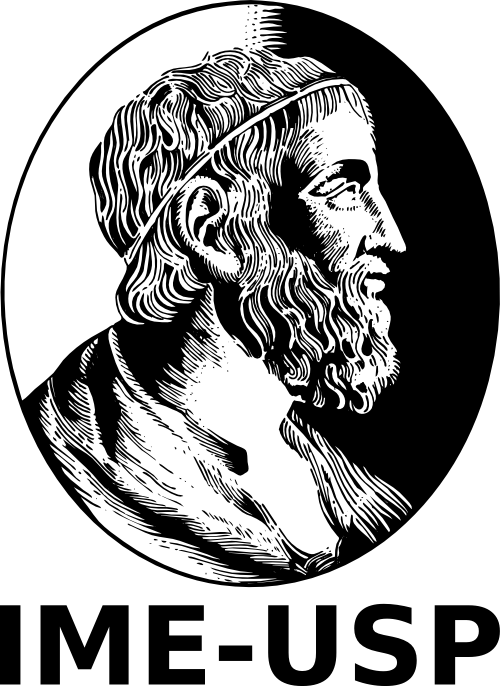
\includegraphics[width=0.25\textwidth]{picstcc/ime.png}
  \end{figure}}
   \vspace{0.4cm}
 \end{center}
  \end{titlepage}

\chapter*{Objetivo}
\textbf{Magic: The Gathering} é um jogo de cartas criado em 1993 por
Richard Garfield que introduziu o conceito moderno de \textit{trading
card game} (jogo de cartas colecionáveis). Com um acervo de mais de 15
mil cartas diferentes, os jogadores devem criar baralhos de 60 cartas
(normalmente podendo haver repetição de até quatro cartas iguais) e
competir, normalmente em jogos um contra um.
\par Durante o jogo, os jogadores têm que lidar com informações
conhecidas (as cartas já jogadas previamente e as cartas em suas mãos) e
informações desconhecidas (as cartas na mão de seu oponente e a ordem
das cartas em seu baralho), o que faz com que seja praticamente
impossível ter informação perfeita. Além disso, ambos os jogadores podem
agir a praticamente qualquer momento dentro de um turno, o que adiciona
uma camada a mais de complexidade.
\par Já existem inteligências artificiais feitas para jogar
\textbf{Magic}, mas devido à complexidade do jogo, nenhuma inteligência
artificial consegue ser realmente boa no jogo (por exemplo, elas não
costumam levar em consideração as cartas que estão na sua mão, então é
muito fácil fazer com que a IA sempre ``morda sua isca'').
\par Nosso objetivo com o trabalho será entender o problema e criar a
nossa versão de uma inteligência artificial para uma versão simplificada
do jogo (limitando o conjunto de cartas disponíveis, adicionando
restrições à construção dos baralhos e simplificando algumas regras do
jogo).

\chapter{Introdução}

Inteligência artificial é um campo da ciência da computação que estuda
``agentes inteligentes'', que de certa forma percebem o ambiente à sua volta
e tomam ações tendo como objetivo maximizar a chance de sucesso de alguma
tarefa específica. Uma utilização muito comum nos dias de hoje é a de
inteligência artificial com o objetivo de criar um agente capaz de competir
com humanos em jogos com alto nível de estratégia, como Xadrez e Go.
Decidimos então estudar inteligência artificial para a realização deste
trabalho com a ideia de modelar um outro jogo de estratégia,
\textbf{Magic: The Gathering}.

\textbf{Magic} foi lançado em 1993, introduzindo o conceito de trading card
game. Com o sucesso do jogo e popularização dos jogos digitais, eventualmente
nasceram versões digitais do jogo para computadores e videogames, e com isso
nasceu a necessidade de agentes que jogassem contra os jogadores. Atualmente
há várias versões digitais de \textbf{Magic}, mas nenhuma tem uma inteligência artificial
boa o suficiente para se provar desafiadora contra jogadores experientes, uma vez
que para cada ação há uma grande quantidade de possibilidades e elementos como
blefe envolvidos. Nossa intenção é entender a complexidade da representação do
jogo e criar uma plataforma para jogar \textbf{Magic} que possibilite a implementação de
um agente de inteligência artificial.

Na próxima seção iremos introduzir alguns conceitos e regras básicas do jogo,
de modo a possibilitar a familiarização do leitor com \textbf{Magic}, facilitando
a compreensão do restante do trabalho.

\section{Conceitos básicos}
Um jogo usual de \textbf{Magic: the Gathering} conta com dois jogadores munidos
de um baralho de 60 cartas cada, ambos começando com 20 pontos de vida, sendo
que o objetivo é reduzir o total de pontos de vida do oponente a 0. Para tanto,
é preciso usar as cartas disponíveis na mão, que podem representar feitiços,
criaturas ou terrenos (existem outros tipos de cartas, mas para nossa implementação
iremos focar nesses três).

\subsection{Cartas}

Nesta seção explicamos a estrutura de uma carta e as diferenças entre os três tipos de carta que utilizamos no projeto. Antes de tudo, convém definir alguns termos utilizados no jogo:

\begin{itemize}
  \item \textbf{Jogar} uma carta é um termo genérico para ``retirar uma carta da sua mão e aplicar seus efeitos no jogo''. Dependendo do tipo de uma carta, quando esta é ``jogada'', será colocada no \textit{campo de batalha} (termo próprio para a mesa de jogo) ou no \textit{cemitério} (termo próprio para a pilha de descarte) do jogador. Uma carta na mesa é chamada \textit{permanente}.
  \item \textbf{Virar} (em inglês, \textit{tap}) uma permanente significa fisicamente dispô-la horizontalmente (normalmente uma carta está na posição vertical). Esta ação representa uma espécie de ação das permenentes. Quando o turno começa, o jogador ativo \textit{desvira} suas permanentes (ou seja, as dispõe em posição vertical), portanto, usualmente, virar uma permanente é um movimento que acontecerá em até uma vez (por permanente) durante cada turno.
\end{itemize}

A seguir, examinaremos a estrutura de uma carta.

\begin{figure}[!ht]
    \centering
    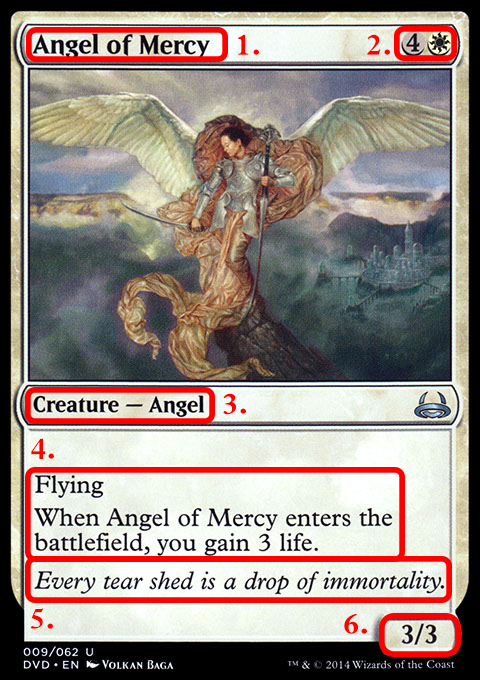
\includegraphics[width=0.7\textwidth]{picstcc/angelnumbers.png}
    \caption{Angel of Mercy e seus principais atributos.}
    \label{cardinfo}
\end{figure}

\begin{enumerate}
  \item \textbf{Nome} da carta.
  \item \textbf{Custo de mana}. ``Mana'' é o recurso necessário em \textbf{Magic} para jogar cartas que não sejam terrenos. Os símbolos da caixa representam a quantidade e tipo de mana necessários para jogar Angel of Mercy.
  $\vcenter{\hbox{
\includegraphics[scale=0.015]{picstcc/4.png}}}$$\vcenter{\hbox{
\includegraphics[scale=0.015]{picstcc/W.png}}}$, então, significa que, para jogar a carta é preciso 4 ``manas'' de qualquer tipo e uma ``mana'' branca, totalizando 5. Mana é geralmente de um dos 5 tipos -- chamados \textit{cores} -- possíveis: Branco ($\vcenter{\hbox{
\includegraphics[scale=0.015]{picstcc/W.png}}}$), Azul, ($\vcenter{\hbox{
\includegraphics[scale=0.015]{picstcc/U.png}}}$), Preto ($\vcenter{\hbox{
\includegraphics[scale=0.015]{picstcc/B.png}}}$), Vermelho ($\vcenter{\hbox{
\includegraphics[scale=0.015]{picstcc/R.png}}}$) e Verde ($\vcenter{\hbox{
\includegraphics[scale=0.015]{picstcc/G.png}}}$). O custo ainda determina a \textit{cor} da própria carta: Angel of Mercy requer apenas mana branca, portanto é uma carta branca.
  \item \textbf{Tipos} de cartas são escritos nesta caixa. Como já mencionado, o tipo de Angel of Mercy é Criatura. Além disso, cartas -- quase sempre criaturas -- também podem ter \textit{subtipos} indicando características da criatura, no caso, um Anjo. Isto é relevante para alguns efeitos do jogo, mas nenhum deles é abordado no projeto.
  \item \textbf{Habilidades} definem os efeitos próprios das cartas. Neste trabalho, usamos apenas criaturas com \textit{habilidades de combate}, características de cada criatura que definem seu comportamento na etapa de combate, e habilidades do tipo ``ao entrar em jogo'', desencadeadas quando a carta se torna uma permanente. \\ No caso, Angel of Mercy tem instâncias dos dois tipos: \textit{Flying} (em portugês, Voar), que limita as interações do oponente durante a etapa de Combate, e sua segunda habilidade, que concede a seu controlador um bônus de 3 pontos de vida. Existem, também, criaturas sem habilidades (porém não existem feitiços sem habilidades). Algumas cartas contêm explicações, em parênteses, de efeitos comuns (como Voar).
  \item \textit{\textbf{Flavor text}} é um texto que ambienta a carta dentro de alguma temática. Pode ser uma fala, um comentário, ou até uma pequena história. \textit{Flavor texts} são escritos em itálico e não influenciam em nada as regras do jogo.
  \item Esta caixa contém os atributos mais importantes das criaturas (e presentes apenas neste tipo de carta): \textbf{poder e resistência}. $X/Y$ representa uma criatura com poder $X$ e resistência $Y$, ou seja, na etapa de combate, esta criatura causa $X$ de dano total e, a qualquer momento, se a criatura tiver uma quantidade $d$ de dano marcado tal que $d \ge Y$, a criatura é destruída.
\end{enumerate}
Os \textbf{terrenos} citados são responsáveis por gerar mana para jogar cartas com custo. Para jogar um terreno, o jogador ativo simplesmente o retira da sua mão e coloca em campo (podendo fazer isso no máximo uma vez por turno). Neste trabalho usamos apenas terrenos com o supertipo \textit{Básico}.\footnote{Geralmente, em \textbf{Magic}, um baralho tem a limitação de 4 cópias de uma mesma carta. Cartas com o supertipo \textit{Básico} não são afetadas por esta limitação.} A cor da mana gerada pelo terreno está ligada a seu subtipo e seu símbolo associado também aparece na carta. Todos os terrenos básicos têm a habilidade ``$\vcenter{\hbox{
\includegraphics[scale=0.015]{picstcc/T.png}}}$: adicione $C$ à sua reserva de mana.'', onde $C \in \left\{ \vcenter{\hbox{
\includegraphics[scale=0.015]{picstcc/W.png}}}, \vcenter{\hbox{
\includegraphics[scale=0.015]{picstcc/U.png}}}, \vcenter{\hbox{
\includegraphics[scale=0.015]{picstcc/B.png}}}, \vcenter{\hbox{
\includegraphics[scale=0.015]{picstcc/R.png}}}, \vcenter{\hbox{
\includegraphics[scale=0.015]{picstcc/G.png}}}\right\}$, não escrita na carta.
\begin{figure}[!h]
  \centering
  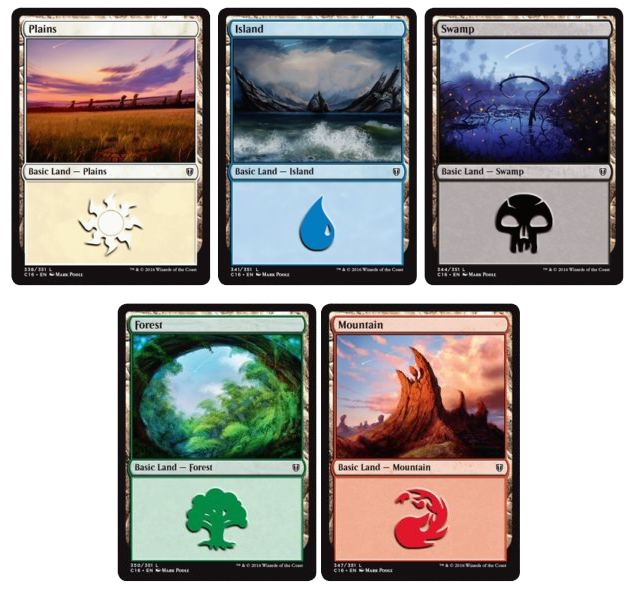
\includegraphics[width=0.7\textwidth]{picstcc/basiclands.png}
  \caption{Os cinco terrenos básicos. Em sentido horário: Planície, Ilha, Pântano, Montanha, Floresta.}
  \label{basiclands}
\end{figure}
\vskip1ex

Assim, a rotina para jogar uma carta com determinado custo é virar o número de terrenos necessários de cada tipo, remover a carta da mão e aplicar seus efeitos (caso seja uma Criatura, é colocada em campo e se torna uma Permanente, caso seja um Feitiço, seus efeitos são aplicados e é colocada no cemitério). No caso de Angel of Mercy, o jogador deve virar 4 terrenos quaisquer e uma Planície para jogá-la. Assim, que o anjo entrar em jogo, seu efeito é desencadeado Apesar de ser possível (e usual) usar mais de uma cor em um baralho, para este trabalho trabalharemos com baralhos de só uma cor.

\begin{figure}[!h]
  \centering
  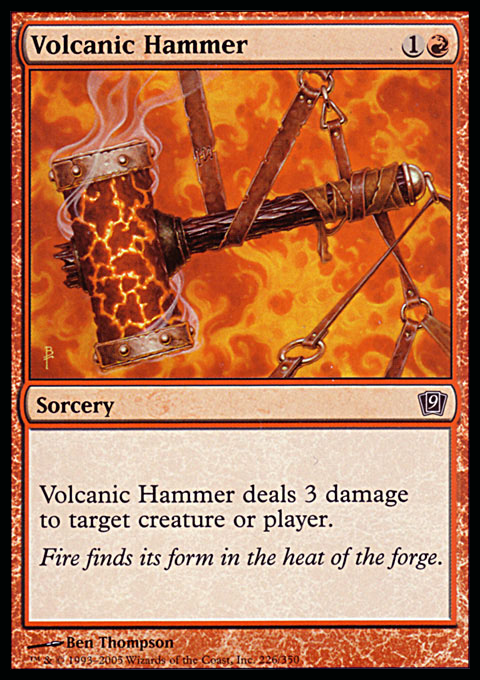
\includegraphics[width=0.5\textwidth]{picstcc/volcanicfull.png}
  \caption{O Feitiço ``Volcanic Hammer'' (Martelo Vulcânico)}
  \label{volcanicsorcery}
\end{figure}

A figura \ref{volcanicsorcery} contém, enfim, um exemplo de Feitiço. A carta possui todas as características de uma carta de Criatura, exceto pelo poder e resistência. Para jogar Volcanic Hammer, além de virar o número de terrenos necesário (ou seja, uma Montanha e um terreno qualquer para pagar o custo de $\vcenter{\hbox{
\includegraphics[scale=0.015]{picstcc/1.png}}} \vcenter{\hbox{
\includegraphics[scale=0.015]{picstcc/R.png}}}$), o jogador ativo deve eleger um \textbf{alvo} para o efeito da carta. O próprio efeito descreve os alvos legais -- no caso, o alvo escolhido pode ser qualquer criatura em campo \textit{ou} qualquer jogador. Alguns efeitos tem seus alvos restritos, por exemplo, a criaturas do oponente ou somente a jogadores.

\vskip1ex

\label{gamestructure}

No começo do jogo é decidido aleatoriamente quem será o jogador inicial,
e então os dois jogadores compram uma mão inicial de sete cartas.
Antes do jogo propriamente dito começar, os jogadores podem optar por tomar uma
ação chamada \textit{mulligan}, que consiste em rejeitar a mão inicial, embaralhá-la
de volta com o restante dos cards e comprar uma nova mão inicial, com uma carta
a menos. Pode-se então repetir o processo até que cada jogador esteja satisfeito
com a mão inicial ou até o jogador realizar um mulligan com apenas uma carta na
mão (resultando em uma mão de zero cartas, onde não há mais a possibilidade de
realizar mulligan). Uma vez que os dois jogadores tiverem escolhido manter uma
mão inicial, cada jogador que realizou pelo menos um mulligan olha a carta do
topo de seu \textit{deck} (como é chamado o baralho) e decide se quer colocá-la
no fundo.

\vskip1ex

O jogo então começa, com os jogadores alternando entre turnos, onde o
jogador que ``controla o turno'' é chamado de \textit{jogador ativo},
com a seguinte estrutura, simplificada:

\begin{itemize}
    \item\textbf{Início do turno}: Permanentes do jogador ativo são
desviradas. Jogador ativo compra uma carta de seu deck.
    \item\textbf{Primeira Fase Principal}: Jogador ativo pode jogar as
cartas da mão. Termina quando o jogador ativo decide \textit{passar}, o que implica no término da fase atual.
    \item \textbf{Combate}: O combate é a maneira principal de um jogador ganhar o jogo, pois envolve a tentativa de diminuição dos pontos de vida de seu oponente através de ataques de suas criaturas. Será melhor explicado na próxima seção.
    \item \textbf{Segunda Fase Principal}: Igual à primeira Fase Principal.
    \item \textbf{Fase final}: Todas as criaturas tem seu dano marcado revertido para 0. Caso o jogador tenha mais de sete cartas na mão, deve descartar (colocar no \textit{cemitério}) até ter uma mão de sete cartas.
\end{itemize}

A estrutura acima se repete até o jogo terminar, o que acontece
geralmente quando algum jogador chega a 0 pontos de vida,
mas também pode acontecer de outras maneiras como, por exemplo, se o
baralho de um jogador acabar.

\subsection{Exemplo de Fases Principais}

Suponhamos que o jogador ativo tem 5 Planícies desviradas e 20 pontos de vida. Na sua primeira Fase Principal, joga seu Angel of Mercy (virando as 5 planícies para adicionar $\vcenter{\hbox{
\includegraphics[scale=0.015]{picstcc/W.png}}} \vcenter{\hbox{
\includegraphics[scale=0.015]{picstcc/W.png}}}\vcenter{\hbox{
\includegraphics[scale=0.015]{picstcc/W.png}}}\vcenter{\hbox{
\includegraphics[scale=0.015]{picstcc/W.png}}}\vcenter{\hbox{
\includegraphics[scale=0.015]{picstcc/W.png}}}$ à sua reserva de mana), que tem seu efeito desencadeado levando-o a 23 pontos de vida. Decide, então, passar o turno para a fase de Combate. Como não tem nenhuma criatura apta a atacar (melhor explicado na próxima subseção), a fase de Combate termina e começa a segunda Fase Principal. O jogador ativo decide passar a segunda fase principal. No próximo turno, o jogador ativo é trocado, compra uma carta e inicia sua primeira Fase Principal. O (novo) jogador ativo tem duas montanhas e decide jogar Volcanic Hammer alvejando Angel of Mercy (e para fazê-lo, vira as duas montanhas, gerando $\vcenter{\hbox{
\includegraphics[scale=0.015]{picstcc/1.png}}} \vcenter{\hbox{
\includegraphics[scale=0.015]{picstcc/R.png}}}$). Como o anjo tem 3 de resistência e o Feitiço lhe causa 3 dano, a permanente é destruída.

\subsection{Combate}

A fase de Combate é a principal maneira do jogador ativo diminuir o total de vida de seu oponente. Isto é realizado ao \textbf{atacar} com suas criaturas. O jogador defensor, como é chamado o oponente do jogador ativo, tem a chance de \textbf{bloquear} os ataques com as suas próprias criaturas. A maioria dos jogos de \textbf{Magic} termina durante esta fase.

\begin{enumerate}
  \item Jogador ativo \textit{declara atacantes} -- escolhe
quais de suas criaturas irão atacar seu oponente. Uma criatura só pode atacar se 1) estiver \textbf{desvirada} (representada na posição vertical) e 2) não estiver \textit{enjoada} (termo que significa que a criatura entrou em jogo neste turno -- uma criatura só pode atacar a partir do turno seguinte ao turno que entrou no campo de batalha). Uma vez que o jogador decidiu com quais criaturas atacar, deve \textbf{virar} as criaturas declaradas para indicar que estas estão atacando. Se o jogador ativo não tiver criaturas aptas a atacar (ou decidir não atacar com nenhuma), a fase de Combate termina.
    \item O jogador defensor \textit{declara bloqueadores} -- escolhe quais de suas criaturas irão
bloquear as criaturas atacantes. Mais uma vez, apenas criaturas \textbf{desviradas} podem bloquear. Diferentemente das criaturas atacantes, porém, criaturas bloqueadoras \textbf{não} se tornam viradas por executar essa ação. Algumas habilidades restringem como criaturas podem bloquear: uma criatura atacante com Voar só pode ser bloqueada por criaturas com a habilidade Voar ou Alcance (\textit{Reach}).
    \item Caso alguma criatura atacante esteja bloqueada
por mais de uma criatura, o jogador ativo decide, então, a ordem com que o dano será
atribuído a cada criatura bloqueadora.
    \item Por fim, há a atribuição de dano. Cada criatura atacante causa dano igual a seu poder às criaturas que a bloqueiam e, caso, não esteja bloqueada, causa dano igual ao seu poder ao jogador defensor. Cada criatura bloqueadora causa dano igual ao seu poder à criatura que bloqueou.
\end{enumerate}

\subsection{Exemplo de Combate}

Suponhamos que o jogador ativo tenha três criaturas desviradas e não-enjoadas no início da fase de combate e seu oponente tenha duas criaturas desviradas (portanto, aptas a bloquear) e 20 pontos de vida.

\begin{figure}[!h]
  \centering
  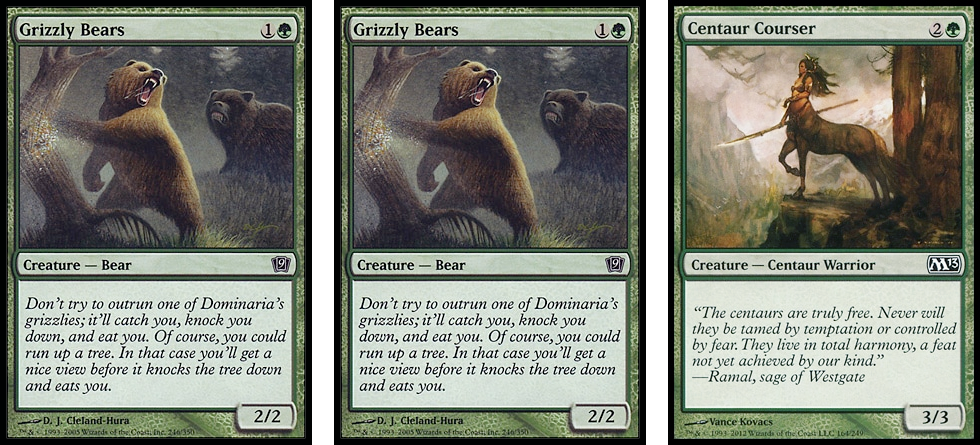
\includegraphics[width=0.8\textwidth]{picstcc/att1.png}
  \caption{Criaturas do jogador ativo: dois ``Grizzly Bears'' (Ursos Cinzentos) em uma ``Centaur Courser'' (Centaura-Caçadora).}
  \label{beginattack}
\end{figure}

\newpage

\begin{figure}[!h]
  \centering
  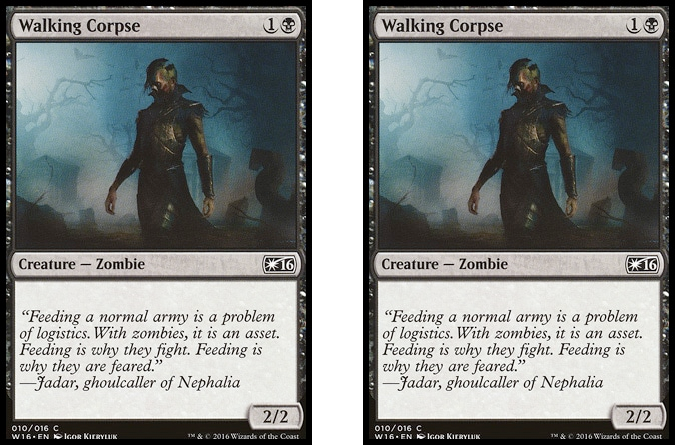
\includegraphics[width=0.55\textwidth]{picstcc/blk1.png}
  \caption{Criaturas do jogador defensor: dois ``Walking Corpse'' (Cadáver Ambulante).}
  \label{beginblock}
\end{figure}

Supondo que o jogador ativo decida atacar com Centaur Courser e um Grizzly Bears, deve então virá-los.

\begin{figure}[!h]
  \centering
  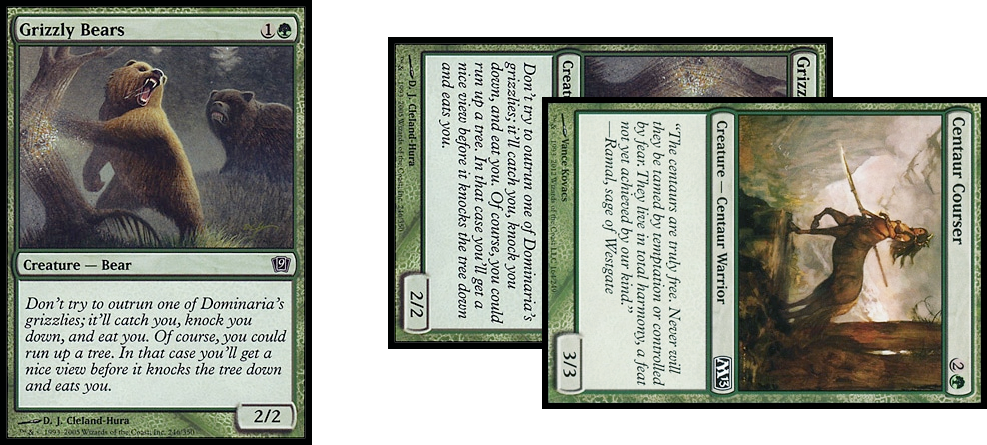
\includegraphics[width=0.8\textwidth]{picstcc/att2.png}
  \caption{Ataque submetido pelo jogador ativo.}
  \label{declaredattackers}
\end{figure}

\newpage

Por fim, o jogador defensor deve declarar quais de suas criaturas bloquearão a ofensiva. Suponhamos, então, que a escolha seja apenas bloquear Grizzly Bears com um Walking Corpse.

\begin{figure}[!h]
  \centering
  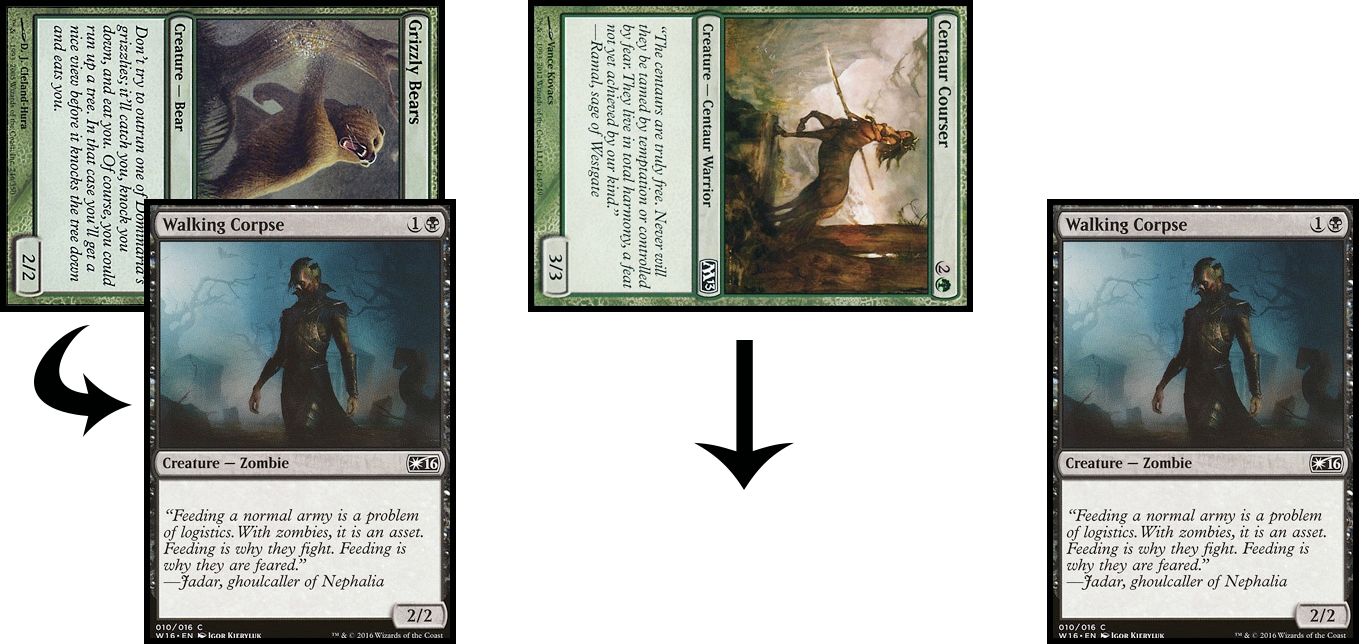
\includegraphics[width=0.8\textwidth]{picstcc/blk2.png}
  \caption{Representação dos bloqueios.}
  \label{declaredblockers}
\end{figure}

Assim, no final do combate, Grizzly Bears causa 2 de dano a Walking Corpse, que por sua vez também lhe causa 2 de dano. Ambas as criaturas são destruídas. Centaur Courser causa 3 de dano ao jogador defensor. O jogador defensor termina 17 de vida e um Walking Corpse desvirado, enquanto o jogador ativo tem 20 de vida e um Centaur Courser virado.


\chapter{Implementação do Cliente}
Para que fosse possível que implementássemos um agente de inteligência artificial que
jogasse uma versão simplificada de Magic, era essencial que conhecêssemos em detalhe a
plataforma onde o jogo estaria rodando, e para isso implementamos do zero uma versão do
jogo com as especifidades desejadas usando a linguagem Python.

O programa é composto de quatro classes principais: \texttt{Game}, \texttt{Player}, \texttt{Card}
e \texttt{Permanent}, representando o Jogo, Jogadores, Cartas e Permanentes (como são tratadas as
cartas de Terreno e Criatura uma vez que estão em jogo) respectivamente. A seguir vamos falar de
cada uma destas classes entrando em detalhes nas principais características.

\section{\texttt{class Card:}}
A classe \texttt{Card} representa as cartas do jogo. Os objetos que estarão presentes nas mãos,
decks e cemitérios dos jogadores serão classes que herdam desta classe. Seus atributos representam
características presentes em todas as cartas. Para exemplificar os atributos, usaremos as cartas mostradas no capítulo anterior: Volcanic Hammer e Angel of Mercy. Os atributos a seguir são comuns a todos os tipos de carta, e por isso estão presentes na
classe Card:

\begin{itemize}
  \item\texttt{name}: Uma string representando o nome da carta, por exemplo ``Volcanic Hammer''
  ou ``Angel of Mercy''.
  \item\texttt{cost}: Uma string representando o custo de mana da carta, usando a mesma notação
  presente nas cartas, com W, U, B, R e G representando os símbolos de mana $\vcenter{\hbox{
\includegraphics[scale=0.015]{picstcc/W.png}}}$ (Branco), $\vcenter{\hbox{
\includegraphics[scale=0.015]{picstcc/U.png}}}$ (Azul),
  $\vcenter{\hbox{
\includegraphics[scale=0.015]{picstcc/B.png}}}$ (Preto),
  $\vcenter{\hbox{
\includegraphics[scale=0.015]{picstcc/R.png}}}$ (Vermelho) e $\vcenter{\hbox{
\includegraphics[scale=0.015]{picstcc/G.png}}}$ (Verde) respectivamente. No caso de Volcanic Hammer, o custo é ``1R'' e no de Angel of Mercy, ``4W''.
  \item\texttt{supertype}: Uma string representando o supertipo da carta. No nosso programa,
  o único supertipo que irá aparecer é \texttt{'Basic'}``Basic'', que identifica os terrenos básicos, mas essa
  informação não é relevante para o programa. Estamos representando essa informação principalmente por formalidade para que o programa siga a mesma estrutura de tipos descrita nas regras do jogo. Nem Volcanic Hammer nem Angel of Mercy
  possuem supertipos, portanto este atributo é representado pela string vazia.
  \item\texttt{ctype}: Uma string que representa o tipo da carta. Angel of Mercy recebe o tipo
  \texttt{'Creature'} e Volcanic Hammer,\texttt{'Sorcery'}. Diferentemente de supertipo ou subtipo,
  este é um atributo que nunca estará vazio em uma carta.
  \item\texttt{subtype}: Uma string que representa o subtipo da carta. O subtipo serve para que
  algumas cartas tenham uma informação adicional que possa ser usada para ações dentro do jogo.
  Volcanic Hammer não tem subtipo, enquanto o subtipo de Angel of Mercy recebe \texttt{'Angel'}.
  \item\texttt{text}: Uma string representando o texto da carta. Essa string serve somente para
  interface com o jogador. O texto de Volcanic Hammer é ``Volcanic Hammer deals 3 damage to target
  creature or player.'' enquanto o de Angel of Mercy é ``Flying. When Angel of Mercy enters the
  battlefield, you gain 3 life. 3/3''.
  \item\texttt{targets}: Uma lista contendo tuplas com as possibilidades de alvo que a carta
  pode ter. Angel of Mercy não tem alvos, e portanto sua lista de alvos é vazia. Volcanic Hammer
  pode dar alvo em criaturas ou jogadores, então sua lista de alvos é
  \texttt{[(``OwnCreature'', ``OpponentCreature'', ``Player'')]}. Separamos criaturas  entre
  criaturas do mesmo dono da carta ou criaturas dos oponentes pois há cartas que só podem ter
  um destes conjuntos como alvo, facilitando a implementação.
  \item\texttt{owner}: O jogador dono da carta. Este atributo é do tipo \texttt{Player}.
\end{itemize}
Para cada carta com nome diferente, há uma classe que herda da classe \texttt{Card} e implementa
as especificidades da carta. Vejamos o código da classe \texttt{VolcanicHammer}, que implementa
a carta Volcanic Hammer:
\begin{figure}
  \begin{Verbatim}[commandchars=\\\{\}]
\PY{k}{class} \PY{n+nc}{VolcanicHammer}\PY{p}{(}\PY{n}{Card}\PY{p}{)}\PY{p}{:}
    \PY{k}{def} \PY{n+nf+fm}{\PYZus{}\PYZus{}init\PYZus{}\PYZus{}}\PY{p}{(}\PY{n+nb+bp}{self}\PY{p}{,} \PY{n}{owner}\PY{p}{)}\PY{p}{:}
        \PY{n+nb+bp}{self}\PY{o}{.}\PY{n}{name} \PY{o}{=} \PY{l+s+s2}{\PYZdq{}}\PY{l+s+s2}{Volcanic Hammer}\PY{l+s+s2}{\PYZdq{}}
        \PY{n+nb+bp}{self}\PY{o}{.}\PY{n}{cost} \PY{o}{=} \PY{l+s+s2}{\PYZdq{}}\PY{l+s+s2}{1R}\PY{l+s+s2}{\PYZdq{}}
        \PY{n+nb+bp}{self}\PY{o}{.}\PY{n}{supertype} \PY{o}{=} \PY{l+s+s2}{\PYZdq{}}\PY{l+s+s2}{\PYZdq{}}
        \PY{n+nb+bp}{self}\PY{o}{.}\PY{n}{ctype} \PY{o}{=} \PY{l+s+s2}{\PYZdq{}}\PY{l+s+s2}{Sorcery}\PY{l+s+s2}{\PYZdq{}}
        \PY{n+nb+bp}{self}\PY{o}{.}\PY{n}{subtype} \PY{o}{=} \PY{l+s+s2}{\PYZdq{}}\PY{l+s+s2}{\PYZdq{}}
        \PY{n+nb+bp}{self}\PY{o}{.}\PY{n}{text} \PY{o}{=} \PY{l+s+s2}{\PYZdq{}}\PY{l+s+s2}{Volcanic Hammer deals 3 damage to target creature or player.}\PY{l+s+s2}{\PYZdq{}}
        \PY{n+nb+bp}{self}\PY{o}{.}\PY{n}{targets} \PY{o}{=} \PY{p}{[}\PY{p}{[}\PY{l+s+s2}{\PYZdq{}}\PY{l+s+s2}{OwnCreature}\PY{l+s+s2}{\PYZdq{}}\PY{p}{,} \PY{l+s+s2}{\PYZdq{}}\PY{l+s+s2}{OpponentCreature}\PY{l+s+s2}{\PYZdq{}}\PY{p}{,} \PY{l+s+s2}{\PYZdq{}}\PY{l+s+s2}{Player}\PY{l+s+s2}{\PYZdq{}}\PY{p}{]}\PY{p}{]}
        \PY{n+nb+bp}{self}\PY{o}{.}\PY{n}{owner} \PY{o}{=} \PY{n}{owner}

    \PY{k}{def} \PY{n+nf}{effect}\PY{p}{(}\PY{n+nb+bp}{self}\PY{p}{,} \PY{n}{game}\PY{p}{,} \PY{n}{targets}\PY{p}{)}\PY{p}{:}
        \PY{n}{targets}\PY{p}{[}\PY{l+m+mi}{0}\PY{p}{]}\PY{o}{.}\PY{n}{takeDamage}\PY{p}{(}\PY{l+m+mi}{3}\PY{p}{)}
\end{Verbatim}

\end{figure}
Podemos ver que a classe tem o método \texttt{effect()}, que implementa o efeito da carta,
fazendo com que o alvo escolhido sofra três pontos de dano. Vejamos agora a implementação
da carta Angel of Mercy:
\begin{figure}
  
\begin{Verbatim}[commandchars=\\\{\}]
\PY{k}{class} \PY{n+nc}{AngelofMercy}\PY{p}{(}\PY{n}{Card}\PY{p}{)}\PY{p}{:}
    \PY{k}{def} \PY{n+nf+fm}{\PYZus{}\PYZus{}init\PYZus{}\PYZus{}}\PY{p}{(}\PY{n+nb+bp}{self}\PY{p}{,}\PY{n}{owner}\PY{p}{)}\PY{p}{:}
        \PY{n+nb+bp}{self}\PY{o}{.}\PY{n}{name} \PY{o}{=} \PY{l+s+s2}{\PYZdq{}}\PY{l+s+s2}{Angel of Mercy}\PY{l+s+s2}{\PYZdq{}}
        \PY{n+nb+bp}{self}\PY{o}{.}\PY{n}{cost} \PY{o}{=} \PY{l+s+s2}{\PYZdq{}}\PY{l+s+s2}{4W}\PY{l+s+s2}{\PYZdq{}}
        \PY{n+nb+bp}{self}\PY{o}{.}\PY{n}{supertype} \PY{o}{=} \PY{l+s+s2}{\PYZdq{}}\PY{l+s+s2}{\PYZdq{}}
        \PY{n+nb+bp}{self}\PY{o}{.}\PY{n}{ctype} \PY{o}{=} \PY{l+s+s2}{\PYZdq{}}\PY{l+s+s2}{Creature}\PY{l+s+s2}{\PYZdq{}}
        \PY{n+nb+bp}{self}\PY{o}{.}\PY{n}{subtype} \PY{o}{=} \PY{l+s+s2}{\PYZdq{}}\PY{l+s+s2}{Angel}\PY{l+s+s2}{\PYZdq{}}
        \PY{n+nb+bp}{self}\PY{o}{.}\PY{n}{text} \PY{o}{=} \PY{l+s+s2}{\PYZdq{}}\PY{l+s+s2}{Flying. When Angel of Mercy enters the battlefield, you gain 3 life. 3/3}\PY{l+s+s2}{\PYZdq{}}
        \PY{n+nb+bp}{self}\PY{o}{.}\PY{n}{abilities} \PY{o}{=} \PY{p}{[}\PY{l+s+s2}{\PYZdq{}}\PY{l+s+s2}{Flying}\PY{l+s+s2}{\PYZdq{}}\PY{p}{]}
        \PY{n+nb+bp}{self}\PY{o}{.}\PY{n}{targets} \PY{o}{=} \PY{p}{[}\PY{p}{]}
        \PY{n+nb+bp}{self}\PY{o}{.}\PY{n}{owner} \PY{o}{=} \PY{n}{owner}
        \PY{n+nb+bp}{self}\PY{o}{.}\PY{n}{power} \PY{o}{=} \PY{l+m+mi}{3}
        \PY{n+nb+bp}{self}\PY{o}{.}\PY{n}{tou} \PY{o}{=} \PY{l+m+mi}{3}

    \PY{k}{def} \PY{n+nf}{effect}\PY{p}{(}\PY{n+nb+bp}{self}\PY{p}{,} \PY{n}{game}\PY{p}{,} \PY{n}{targets}\PY{p}{)}\PY{p}{:}
        \PY{n+nb+bp}{self}\PY{o}{.}\PY{n}{owner}\PY{o}{.}\PY{n}{gainLife}\PY{p}{(}\PY{l+m+mi}{3}\PY{p}{)}
\end{Verbatim}

\end{figure}
Além dos atributos que citamos anteriormente, Angel of Mercy tem três atributos a mais por
ser do tipo Criatura: \texttt{abilities}, uma lista com as habilidades de combate da criatura;
\texttt{power}, o poder da criatura; e \texttt{tou}, a resistência (toughness) da criatura.
Podemos também ver o efeito da carta, que concede três pontos de vida a seu controlador. O método \texttt{effect} de cada carta é chamado quando esta é jogada, tendo consequências distintas para cada caso.

\section{\texttt{class Permanent:}}
A classe \texttt{Permanent} serve para representar as cartas uma vez que foram jogadas
e estão no campo de batalha. Seus atributos são os seguintes:
\begin{itemize}
  \item\texttt{card}: A carta que criou a permanente. Ela contém informações relevantes
  para a construção do objeto e é ela, e não a permanente, que será colocada no cemitério
  caso deixe o campo de batalha.
  \item\texttt{abilities}: Uma cópia do atributo \texttt{abilities} da carta. É necessário
  que esse atributo seja armazenado separadamente ao da carta, pois uma vez em jogo, a
  permanente pode ganhar ou perder habilidades.
  \item\texttt{ctype}: O tipo da permanente, conforme descrito na carta que a criou.
  \item\texttt{owner}: O jogador dono da permanente, que será o mesmo que possúi a carta.
  \item\texttt{controller}: O jogador controlador da permanente. Normalmente ele será o dono,
  mas há efeitos que mudam o jogador que controla uma permanente.
  \item\texttt{tapped}: Um atributo booleano que indica se a permanente está virada ou
  desvirada.
  \item\texttt{sick}: Um atributo booleano que indica se a permanente está
  \textit{enjoada}\footnote{Permanentes entram em jogo com \textit{enjoo de invocação}, o que
  indica que caso ela seja uma criatura, não poderá atacar. O enjoo de uma permanente acaba no
  começo do turno de seu controlador.} ou não.
  \item\texttt{destroyed}: Um atributo booleano que indica se a permanente foi destruída ou não.
  Permanentes destruídas são colocadas no cemitério de seu controlador durante as checagens do jogo.
  \item\texttt{ID}: Um inteiro que serve como identificador único entre permanentes. Ele serve,
  por exemplo, para diferenciar permanentes que tenham sido criadas a partir de cartas iguais.
\end{itemize}
Estes atributos são alterados a partir dos métodos da classe, que não entraremos em detalhes.

Há duas classes que herdam da classe \texttt{Permanent}: \texttt{Land} e \texttt{Creature}.
\texttt{Land} é a classe que representa terrenos. A única diferença desta classe para a classe
mãe é que os métodos de virar e desvirar manipulam um atributo do jogador controlador: a quantidade
de terrenos desvirados controlados por aquele jogador. A classe \texttt{Creature} tem alguns
atributos a mais:
\begin{itemize}
  \item\texttt{power}: Um inteiro que representa o poder da criatura.
  \item\texttt{tou}: Um inteiro que representa a resistência da criatura.
  \item\texttt{curPower}: Um inteiro que representa o poder atual da criatura. Existem efeitos
  que modificam o poder com duração limitada a um turno. Nestes casos, o poder volta a ser o
  poder armazenado no atributo \texttt{power} quando o próximo turno começar.
  \item\texttt{curTou}: Um inteiro que representa a resistência atual da criatura. Análogo ao
  atributo \texttt{curPower} relativo à resistência da criatura.
  \item\texttt{attacking}: Um atributo booleano que representa se a criatura está atacando
  ou não.
  \item\texttt{blocking}: Um atributo booleano que representa se a criatura está bloqueando
  ou não.
  \item\texttt{damage}: Um inteiro que armazena a quantidade de dano sofrida pela criatura até
  o presente momento. No início de cada turno, este atributo volta a ter o valor $0$.
  \item\texttt{currentAbilities}: Análogo ao atributo \texttt{curPower} para as habilidades.
\end{itemize}
Criaturas têm alguns métodos especiais que possibilitam com que elas realizem ações dentro
do jogo, como atacar ou causar dano, mas não entraremos em detalhes.

\section{\texttt{class Game:}}
A classe \texttt{Game} representa um jogo em andamento. Devido à complexidade da classe, entrar
em detalhes iria mudar o foco do trabalho, então não iremos descrever todos os métodos e atributos
da classe. Há um método chamado \texttt{turnRoutine()} que é chamado repetidamente até que o jogo
termine. Ele executa as ações iniciais e finais do turno (como fazer com que o jogador ativo compre
uma carta no começo do turno e limpar o dano das criaturas no final do turno) e chama os métodos de
fase principal e de combate, que permitem que os jogadores joguem as cartas da mão, ataquem e
bloqueiem.
\vskip1ex
Além disso, há alguns métodos para definir quais são as ações legais para um jogador e para realizar
as chamades \textit{ações baseadas no estado}, que são ações performadas pelo jogo sempre que uma
certa condição baseada no estado do jogo se torna verdade (por exemplo, destruir criaturas com dano
igual ou superior à resistência, fazer com que jogadores com $0$ ou menos pontos de vida percam o
o jogo, e assim por diante). O método que cuida disso é \texttt{checkSBA()} (de ``state based actions''),
chamado pela classe \texttt{Game} nos seguintes momentos:
\begin{itemize}
  \item No início e fim de cada fase.
  \item Após toda ação de Fase Principal.
  \item Durante etapas de atribuição de dano no Combate.
\end{itemize}
\texttt{Game} é responsável por chamar métodos que requerem a decisão do jogador.
\section{\texttt{class Player:}}
A classe \texttt{Player} representa um jogador na partida. Seus atributos são:
\begin{itemize}
  \item\texttt{name}: Uma string representando o nome do jogador. Não tem nenhuma função
  dentro do jogo. Serve para identificar os jogadores na saída.
  \item\texttt{life}: Um inteiro representando o valor atual do total de pontos de vida
  do jogador.
  \item\texttt{hand}: Uma lista de objetos do tipo \texttt{Card}, representando as cartas
  na mão do jogador.
  \item\texttt{library}: Uma lista de objetos do tipo \texttt{Card}, representando as cartas
  no deck\footnote{Dentro do jogo, o deck recebe o nome de \textit{Grimório}, ou \textit{Library},
  em inglês.} do jogador.
  \item\texttt{lose}: Um atributo booleano para identificar se o jogador perdeu o jogo. Este
  atributo é utilizado pela classe \texttt{Game} para decidir se o jogo acabou ou não.
  \item\texttt{ID}: Um inteiro representando um identificador único para o jogador, de maneira
  similar à que acontece com as permanentes.
  \item\texttt{creatures}: Uma lista de objetos da classe \texttt{Creature} com todas as
  criaturas controladas pelo jogador.
  \item\texttt{lands}: Uma lista de objetos da classe \texttt{Land} com todos os terrenos
  controlados pelo jogador.
  \item\texttt{active}: Um atributo booleano que indica se o jogador é o jogador ativo.
  \item\texttt{graveyard}: Uma lista de objetos da classe \texttt{Card} com todas as cartas
  no cemitério do jogador.
  \item\texttt{untappedLands}: Um inteiro representando a quantidade de terrenos desvirados que
  o jogador controla.
  \item\texttt{landDrop}: Um atributo booleano indicando se o jogador já jogou um terreno no
  turno atual.
\end{itemize}

A classe \texttt{Player} representa um jogador \textbf{humano} e possui, dentre outros, os métodos \texttt{mulligan()} \texttt{mainPhaseAction()}, \texttt{declareAttackers()}, \texttt{declareBlockers()}  e \texttt{assignBlockOrder()}que são chamados nas respectivas fases por uma instância de jogo (classe \texttt{Game}). Tais momentos são impressos na saída padrão e esperam uma decisão em texto do jogador.

\begin{figure}[h!]
  \begin{center}
  \begin{Verbatim}
1) Angel of Mercy
2) Inspiring Roar
3) Griffin Sentinel
4) Plains
5) Plains
6) Siege Mastodon
7) Griffin Sentinel
Choose a card from your hand (0 will pass priority, 'p' prints the game state):
  \end{Verbatim}
\end{center}
  \caption{\textit{Prompt} perguntando qual a ação desejada em uma fase principal. \textit{Pass priority} significa passar para a próxima fase. Há prompts análogos para as decisões de mulligan e de combate.}
  \label{mainactionprompt}
\end{figure}

\begin{figure}[!h]
  \centering
  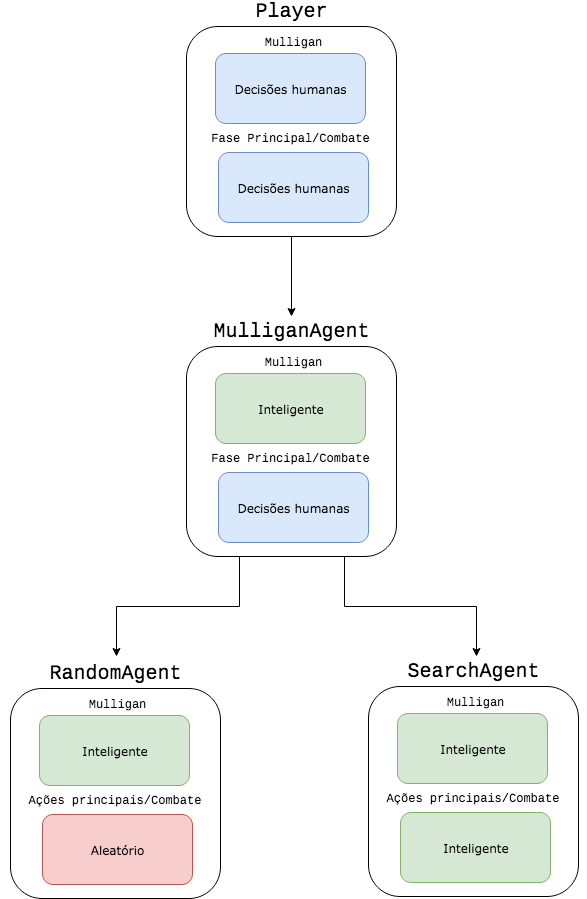
\includegraphics[width=0.6\textwidth]{picstcc/playerdiagram.png}
  \caption{Diagrama de classes de jogadores e agentes.}
  \label{classdiagram}
\end{figure}

Há mais três classes herdadas (diretamente ou não) da classe \texttt{Player}. A primeira delas é \texttt{MulliganAgent}, cuja única diferença funcional em relação a \texttt{Player} é a aplicação de um algoritmo para a decisão automática do mulligan. Um agente \texttt{MulliganAgent} não é 100\% autônomo, pois suas decisões para o resto do jogo ainda são requisitadas ao usuário, e não é chamado pelas opções disponíveis no programa. A existência da classe é justificada pois serve de base para os dois outros agentes (e potencialmente mais): o agente aleatório e o agente inteligente, diferentes entre si. A intenção é que qualquer agente (mesmo aleatório) tenha chance de jogar suas cartas e, para isso, deve definir uma mão inicial suficientemente ``jogável'' (melhor explicado em \ref{sec:mulliganmodel}).
\vskip1ex
A classe \texttt{RandomAgent}, herdada de \texttt{MulliganAgent}, sobrescreve todas as decisões humanas de \texttt{Player} (exceto \texttt{mulligan()}) por métodos que sorteiam e submetem uma ação sorteada dentre a gama de possibilidades. Para isso, usam em cada um de seus métodos um conjunto \texttt{legalActions} de ações legais computado pela instância de \texttt{Game} que os chamou. A obtenção de ações legais é explicada no capítulo \ref{chap:modelagem}.

\vskip1ex
Por fim, a classe \texttt{SearchAgent} também é herdada de \texttt{MulliganAgent} e sobrescreve os métodos de decisões humana por ações decididas por algoritmos. Tais decisões serão examinadas no capítulo \ref{chap:modelagem}.


\newpage
\chapter{Modelagem}
\label{chap:modelagem}

Neste capítulo abordaremos um jogo de \textit{Magic} como um problema de Inteligência Artificial,
mas para explicarmos a modelagem do problema, é necessária a introdução do conceito de Processos
de Decisão de Markov, que é o que usaremos para modelar os problemas do jogo.

\section{Processo De decisão de Markov}
\label{sec:mulliganmodel}

Processos de Decisão de Markov (em inglês, \textit{Markov Decision Process}, ou \textbf{MDP})
são uma forma de representar alguns problemas de decisão sequenciais.

Para descrever um MDP, usaremos um exemplo com o intuito de tornar a explicação mais didática.
Imagine que um gerente de um galpão de um produto tem como objetivo maximizar o lucro esperado
para o próximo ano. A cada mês, o gerente observa quanto há em estoque do produto e decide
quanto irá pedir ao distribuir para o próximo mês. A demanda mensal do produto é desconhecida,
mas segue uma distribuição de probabilidade conhecida. Se o gerente pedir produto demais, terá
custos para manter o estoque, e se pedir de menos, estará perdendo vendas por falta de inventário.
Suponha que o galpão tem capacidade para armazenar $M$ unidades de produto e que os custos e a
distribuição da demanda não muda de mês para mês.

O primeiro conceito de MDP que iremos introduzir é o de \textbf{época de decisão}. Uma época de
decisão é um momento onde uma decisão é tomada. No nosso exemplo, cada época de decisão ocorre
no começo de um mês, quando o gerente deve decidir quanto produto irá pedir ao distribuidor. Chamamos
a quantidade de épocas de decisão de um MDP de \textbf{horizonte}, que pode ser finito ou infinito.
No exemplo, o horizonte é finito de tamanho $12$, sendo uma época para cada mês do ano no qual o
gerente deseja maximizar seus lucros.

Um MDP pode ser representado por uma tupla $(S, A, P, R)$. $S$ é o conjunto de \textbf{estados}
$s_t$ do problema, onde um estado é uma configuração do problema em uma determinada época de
decisão $t$. No exemplo, cada estado representa o espaço disponível no galpão, que pode variar
de $0$ a $M$.

$A$ é o conjunto de \textbf{ações} $a_t$, onde $t$ é a época de decisão. No exemplo, uma ação
pode ser comprar de $0$ a $M-s_t$ unidades no mês.

Para falar sobre os outros elementos da tupla do MDP, precisamos entrar em detalhes sobre os
custos para pedir o produto ao distribuidor e manter o produto em estoque. Um mês começa com $s_t$
unidades em estoque, e são encomendadas mais $a_t$ unidades, o que gera um custo $c_{pedido}$ dado
pela função $c_p(a_t)$. Vamos assumir que as unidades sejam pedidas no começo do mês e sejam vendidas
no final do mês. Há, portanto, um custo $c_{estoque}$ para manter o produto em estoque dado pela função
$c_e(s_t + a_t)$. A probabilidade de que a demanda $D_t$ no mês seja de $j$ unidades é $p_j, j = 0,1,2\ldots$.
Quando o final do mês chegar, o número de unidade vendidas será $x_t = min{D_t, s_t + a_j}$, e o lucro
será dado pela função $l(x_t)$. O número de unidades que começarão o próximo mês em estoque será
$s_{t+1}= s_t + a_t - x_t$.

$R: S \times A \mapsto \mathbb{R}$ é a função que dá a \textbf{recompensa} esperada por tomar a ação $a_t$
quando o processo está no estado estado $s_t$. No exemplo, $r_t(s_t, a_t) = E[l(x_t)] - c_{estoque} - c_{pedido}$.

$P: S \times A \times S \mapsto [0,1]$ é uma função que dá a \textbf{probabilidade} do sistema passar de um estado
para outro, dado uma determinada ação. No nosso exemplo:

\begin{equation*}
  Pr\{s_{t+1} = j|s_t = s, a_t = a\} = \begin{cases}p_{s+a-j} &j\le s + a \\
                                                    \sum\limits_{i=s+a}^\infty &j=0 \\
                                                    0 & j >s+a\end{cases}
\end{equation*}

Uma vez que temos o nosso MDP definido, queremos chegar em uma \textbf{política}, que é o nome dado
ao conjunto das \textbf{regras de decisão}. Uma regra de decisão $d_t(s)$ é uma função $d: S \mapsto A$
que que, dado um estado $s$ na época de decisão $t$, retorna uma ação $a$ que deve ser tomada a partir
daquele estado de modo a maximizar o ganho final. A seguir veremos uma representação de Magic como MDP,
e em seguida como extraímos a política para o processo.

\section{\textit{Mulligan}}
A estrutura de um turno, como descrita no primeiro capítulo, será repetida
algumas vezes até o jogo acabar, porém é necessário determinar a mão inicial de
cada jogador e, por isso, trataremos este problema em separado.
Baseando-se na experiência própria, a estrutura do problema do
\textbf{\textit{mulligan}} é notavelmente diferente do resto de um jogo
de \textit{Magic}.
A principal diferença é que apesar de ambos os jogadores tomarem
decisões alternadamente nessa etapa, as ações do oponente não têm
nenhuma influência
direta sobre as ações do agente, que deve se concentrar em obter uma
\textbf{mão inicial} que possibilite jogadas nos primeiros turnos do
jogo.

\vskip1ex

A figura \ref{mulligan} representa as escolhas que o jogador poderá
fazer para determiná-la, com cada conjunto de cartas representando um
conjunto
de estados.

\begin{figure}
  \centering
  \label{mulligan}
  % Graphic for TeX using PGF
% Title: /home/schutzer/comp/mtcc_super/mtcc_support/mulligan.dia
% Creator: Dia v0.97.3
% CreationDate: Fri Nov 10 11:39:18 2017
% For: schutzer
% \usepackage{tikz}
% The following commands are not supported in PSTricks at present
% We define them conditionally, so when they are implemented,
% this pgf file will use them.
\ifx\du\undefined
  \newlength{\du}
\fi
\setlength{\du}{15\unitlength}
\begin{tikzpicture}[scale=0.35]
\pgftransformxscale{1.000000}
\pgftransformyscale{-1.000000}
\definecolor{dialinecolor}{rgb}{0.000000, 0.000000, 0.000000}
\pgfsetstrokecolor{dialinecolor}
\definecolor{dialinecolor}{rgb}{1.000000, 1.000000, 1.000000}
\pgfsetfillcolor{dialinecolor}
\pgfsetlinewidth{0.100000\du}
\pgfsetdash{}{0pt}
\pgfsetdash{}{0pt}
\pgfsetmiterjoin
\definecolor{dialinecolor}{rgb}{1.000000, 1.000000, 1.000000}
\pgfsetfillcolor{dialinecolor}
\fill (31.000000\du,12.231300\du)--(31.000000\du,19.231300\du)--(36.000000\du,19.231300\du)--(36.000000\du,12.231300\du)--cycle;
\definecolor{dialinecolor}{rgb}{0.000000, 0.000000, 0.000000}
\pgfsetstrokecolor{dialinecolor}
\draw (31.000000\du,12.231300\du)--(31.000000\du,19.231300\du)--(36.000000\du,19.231300\du)--(36.000000\du,12.231300\du)--cycle;
\pgfsetlinewidth{0.100000\du}
\pgfsetdash{}{0pt}
\pgfsetdash{}{0pt}
\pgfsetmiterjoin
\definecolor{dialinecolor}{rgb}{1.000000, 1.000000, 1.000000}
\pgfsetfillcolor{dialinecolor}
\fill (30.000000\du,11.231300\du)--(30.000000\du,18.231300\du)--(35.000000\du,18.231300\du)--(35.000000\du,11.231300\du)--cycle;
\definecolor{dialinecolor}{rgb}{0.000000, 0.000000, 0.000000}
\pgfsetstrokecolor{dialinecolor}
\draw (30.000000\du,11.231300\du)--(30.000000\du,18.231300\du)--(35.000000\du,18.231300\du)--(35.000000\du,11.231300\du)--cycle;
\pgfsetlinewidth{0.100000\du}
\pgfsetdash{}{0pt}
\pgfsetdash{}{0pt}
\pgfsetmiterjoin
\definecolor{dialinecolor}{rgb}{1.000000, 1.000000, 1.000000}
\pgfsetfillcolor{dialinecolor}
\fill (29.000000\du,10.231300\du)--(29.000000\du,17.231300\du)--(34.000000\du,17.231300\du)--(34.000000\du,10.231300\du)--cycle;
\definecolor{dialinecolor}{rgb}{0.000000, 0.000000, 0.000000}
\pgfsetstrokecolor{dialinecolor}
\draw (29.000000\du,10.231300\du)--(29.000000\du,17.231300\du)--(34.000000\du,17.231300\du)--(34.000000\du,10.231300\du)--cycle;
\pgfsetlinewidth{0.100000\du}
\pgfsetdash{}{0pt}
\pgfsetdash{}{0pt}
\pgfsetmiterjoin
\definecolor{dialinecolor}{rgb}{1.000000, 1.000000, 1.000000}
\pgfsetfillcolor{dialinecolor}
\fill (28.000000\du,9.231330\du)--(28.000000\du,16.231330\du)--(33.000000\du,16.231330\du)--(33.000000\du,9.231330\du)--cycle;
\definecolor{dialinecolor}{rgb}{0.000000, 0.000000, 0.000000}
\pgfsetstrokecolor{dialinecolor}
\draw (28.000000\du,9.231330\du)--(28.000000\du,16.231330\du)--(33.000000\du,16.231330\du)--(33.000000\du,9.231330\du)--cycle;
\pgfsetlinewidth{0.100000\du}
\pgfsetdash{}{0pt}
\pgfsetdash{}{0pt}
\pgfsetmiterjoin
\definecolor{dialinecolor}{rgb}{1.000000, 1.000000, 1.000000}
\pgfsetfillcolor{dialinecolor}
\fill (27.000000\du,8.231330\du)--(27.000000\du,15.231330\du)--(32.000000\du,15.231330\du)--(32.000000\du,8.231330\du)--cycle;
\definecolor{dialinecolor}{rgb}{0.000000, 0.000000, 0.000000}
\pgfsetstrokecolor{dialinecolor}
\draw (27.000000\du,8.231330\du)--(27.000000\du,15.231330\du)--(32.000000\du,15.231330\du)--(32.000000\du,8.231330\du)--cycle;
\pgfsetlinewidth{0.100000\du}
\pgfsetdash{}{0pt}
\pgfsetdash{}{0pt}
\pgfsetmiterjoin
\definecolor{dialinecolor}{rgb}{1.000000, 1.000000, 1.000000}
\pgfsetfillcolor{dialinecolor}
\fill (26.000000\du,7.231330\du)--(26.000000\du,14.231330\du)--(31.000000\du,14.231330\du)--(31.000000\du,7.231330\du)--cycle;
\definecolor{dialinecolor}{rgb}{0.000000, 0.000000, 0.000000}
\pgfsetstrokecolor{dialinecolor}
\draw (26.000000\du,7.231330\du)--(26.000000\du,14.231330\du)--(31.000000\du,14.231330\du)--(31.000000\du,7.231330\du)--cycle;
\pgfsetlinewidth{0.100000\du}
\pgfsetdash{}{0pt}
\pgfsetdash{}{0pt}
\pgfsetmiterjoin
\definecolor{dialinecolor}{rgb}{1.000000, 1.000000, 1.000000}
\pgfsetfillcolor{dialinecolor}
\fill (25.000000\du,6.231330\du)--(25.000000\du,13.231330\du)--(30.000000\du,13.231330\du)--(30.000000\du,6.231330\du)--cycle;
\definecolor{dialinecolor}{rgb}{0.000000, 0.000000, 0.000000}
\pgfsetstrokecolor{dialinecolor}
\draw (25.000000\du,6.231330\du)--(25.000000\du,13.231330\du)--(30.000000\du,13.231330\du)--(30.000000\du,6.231330\du)--cycle;
\pgfsetlinewidth{0.100000\du}
\pgfsetdash{}{0pt}
\pgfsetdash{}{0pt}
\pgfsetmiterjoin
\definecolor{dialinecolor}{rgb}{1.000000, 1.000000, 1.000000}
\pgfsetfillcolor{dialinecolor}
\fill (36.000000\du,29.000000\du)--(36.000000\du,36.000000\du)--(41.000000\du,36.000000\du)--(41.000000\du,29.000000\du)--cycle;
\definecolor{dialinecolor}{rgb}{0.000000, 0.000000, 0.000000}
\pgfsetstrokecolor{dialinecolor}
\draw (36.000000\du,29.000000\du)--(36.000000\du,36.000000\du)--(41.000000\du,36.000000\du)--(41.000000\du,29.000000\du)--cycle;
\pgfsetlinewidth{0.100000\du}
\pgfsetdash{}{0pt}
\pgfsetdash{}{0pt}
\pgfsetmiterjoin
\definecolor{dialinecolor}{rgb}{1.000000, 1.000000, 1.000000}
\pgfsetfillcolor{dialinecolor}
\fill (35.000000\du,28.000000\du)--(35.000000\du,35.000000\du)--(40.000000\du,35.000000\du)--(40.000000\du,28.000000\du)--cycle;
\definecolor{dialinecolor}{rgb}{0.000000, 0.000000, 0.000000}
\pgfsetstrokecolor{dialinecolor}
\draw (35.000000\du,28.000000\du)--(35.000000\du,35.000000\du)--(40.000000\du,35.000000\du)--(40.000000\du,28.000000\du)--cycle;
\pgfsetlinewidth{0.100000\du}
\pgfsetdash{}{0pt}
\pgfsetdash{}{0pt}
\pgfsetmiterjoin
\definecolor{dialinecolor}{rgb}{1.000000, 1.000000, 1.000000}
\pgfsetfillcolor{dialinecolor}
\fill (34.000000\du,27.000000\du)--(34.000000\du,34.000000\du)--(39.000000\du,34.000000\du)--(39.000000\du,27.000000\du)--cycle;
\definecolor{dialinecolor}{rgb}{0.000000, 0.000000, 0.000000}
\pgfsetstrokecolor{dialinecolor}
\draw (34.000000\du,27.000000\du)--(34.000000\du,34.000000\du)--(39.000000\du,34.000000\du)--(39.000000\du,27.000000\du)--cycle;
\pgfsetlinewidth{0.100000\du}
\pgfsetdash{}{0pt}
\pgfsetdash{}{0pt}
\pgfsetmiterjoin
\definecolor{dialinecolor}{rgb}{1.000000, 1.000000, 1.000000}
\pgfsetfillcolor{dialinecolor}
\fill (33.000000\du,26.000000\du)--(33.000000\du,33.000000\du)--(38.000000\du,33.000000\du)--(38.000000\du,26.000000\du)--cycle;
\definecolor{dialinecolor}{rgb}{0.000000, 0.000000, 0.000000}
\pgfsetstrokecolor{dialinecolor}
\draw (33.000000\du,26.000000\du)--(33.000000\du,33.000000\du)--(38.000000\du,33.000000\du)--(38.000000\du,26.000000\du)--cycle;
\pgfsetlinewidth{0.100000\du}
\pgfsetdash{}{0pt}
\pgfsetdash{}{0pt}
\pgfsetmiterjoin
\definecolor{dialinecolor}{rgb}{1.000000, 1.000000, 1.000000}
\pgfsetfillcolor{dialinecolor}
\fill (32.000000\du,25.000000\du)--(32.000000\du,32.000000\du)--(37.000000\du,32.000000\du)--(37.000000\du,25.000000\du)--cycle;
\definecolor{dialinecolor}{rgb}{0.000000, 0.000000, 0.000000}
\pgfsetstrokecolor{dialinecolor}
\draw (32.000000\du,25.000000\du)--(32.000000\du,32.000000\du)--(37.000000\du,32.000000\du)--(37.000000\du,25.000000\du)--cycle;
\pgfsetlinewidth{0.100000\du}
\pgfsetdash{}{0pt}
\pgfsetdash{}{0pt}
\pgfsetmiterjoin
\definecolor{dialinecolor}{rgb}{1.000000, 1.000000, 1.000000}
\pgfsetfillcolor{dialinecolor}
\fill (31.000000\du,24.000000\du)--(31.000000\du,31.000000\du)--(36.000000\du,31.000000\du)--(36.000000\du,24.000000\du)--cycle;
\definecolor{dialinecolor}{rgb}{0.000000, 0.000000, 0.000000}
\pgfsetstrokecolor{dialinecolor}
\draw (31.000000\du,24.000000\du)--(31.000000\du,31.000000\du)--(36.000000\du,31.000000\du)--(36.000000\du,24.000000\du)--cycle;
\definecolor{dialinecolor}{rgb}{1.000000, 1.000000, 1.000000}
\pgfsetfillcolor{dialinecolor}
\fill (54.005330\du,14.000000\du)--(56.010660\du,15.752665\du)--(54.005330\du,17.505330\du)--(52.000000\du,15.752665\du)--cycle;
\pgfsetlinewidth{0.100000\du}
\pgfsetdash{}{0pt}
\pgfsetdash{}{0pt}
\pgfsetmiterjoin
\definecolor{dialinecolor}{rgb}{0.000000, 0.000000, 0.000000}
\pgfsetstrokecolor{dialinecolor}
\draw (54.005330\du,14.000000\du)--(56.010660\du,15.752665\du)--(54.005330\du,17.505330\du)--(52.000000\du,15.752665\du)--cycle;
% setfont left to latex
\definecolor{dialinecolor}{rgb}{0.000000, 0.000000, 0.000000}
\pgfsetstrokecolor{dialinecolor}
\node at (54.005330\du,15.947665\du){};
\pgfsetlinewidth{0.100000\du}
\pgfsetdash{}{0pt}
\pgfsetdash{}{0pt}
\pgfsetbuttcap
{
\definecolor{dialinecolor}{rgb}{0.000000, 0.000000, 0.000000}
\pgfsetfillcolor{dialinecolor}
% was here!!!
\pgfsetarrowsend{stealth}
\definecolor{dialinecolor}{rgb}{0.000000, 0.000000, 0.000000}
\pgfsetstrokecolor{dialinecolor}
\draw (36.049399\du,15.733956\du)--(51.950000\du,15.750524\du);
}
\definecolor{dialinecolor}{rgb}{1.000000, 1.000000, 1.000000}
\pgfsetfillcolor{dialinecolor}
\pgfpathellipse{\pgfpoint{70.343600\du}{15.752300\du}}{\pgfpoint{2.500000\du}{0\du}}{\pgfpoint{0\du}{2.500000\du}}
\pgfusepath{fill}
\pgfsetlinewidth{0.100000\du}
\pgfsetdash{}{0pt}
\pgfsetdash{}{0pt}
\pgfsetmiterjoin
\definecolor{dialinecolor}{rgb}{0.000000, 0.000000, 0.000000}
\pgfsetstrokecolor{dialinecolor}
\pgfpathellipse{\pgfpoint{70.343600\du}{15.752300\du}}{\pgfpoint{2.500000\du}{0\du}}{\pgfpoint{0\du}{2.500000\du}}
\pgfusepath{stroke}
% setfont left to latex
\definecolor{dialinecolor}{rgb}{0.000000, 0.000000, 0.000000}
\pgfsetstrokecolor{dialinecolor}
\node at (70.343600\du,15.947300\du){};
\definecolor{dialinecolor}{rgb}{1.000000, 1.000000, 1.000000}
\pgfsetfillcolor{dialinecolor}
\fill (54.005330\du,30.691600\du)--(56.010660\du,32.444265\du)--(54.005330\du,34.196930\du)--(52.000000\du,32.444265\du)--cycle;
\pgfsetlinewidth{0.100000\du}
\pgfsetdash{}{0pt}
\pgfsetdash{}{0pt}
\pgfsetmiterjoin
\definecolor{dialinecolor}{rgb}{0.000000, 0.000000, 0.000000}
\pgfsetstrokecolor{dialinecolor}
\draw (54.005330\du,30.691600\du)--(56.010660\du,32.444265\du)--(54.005330\du,34.196930\du)--(52.000000\du,32.444265\du)--cycle;
% setfont left to latex
\definecolor{dialinecolor}{rgb}{0.000000, 0.000000, 0.000000}
\pgfsetstrokecolor{dialinecolor}
\node at (54.005330\du,32.639265\du){};
\pgfsetlinewidth{0.100000\du}
\pgfsetdash{}{0pt}
\pgfsetdash{}{0pt}
\pgfsetmiterjoin
\definecolor{dialinecolor}{rgb}{1.000000, 1.000000, 1.000000}
\pgfsetfillcolor{dialinecolor}
\fill (40.000000\du,44.000000\du)--(40.000000\du,51.000000\du)--(45.000000\du,51.000000\du)--(45.000000\du,44.000000\du)--cycle;
\definecolor{dialinecolor}{rgb}{0.000000, 0.000000, 0.000000}
\pgfsetstrokecolor{dialinecolor}
\draw (40.000000\du,44.000000\du)--(40.000000\du,51.000000\du)--(45.000000\du,51.000000\du)--(45.000000\du,44.000000\du)--cycle;
\pgfsetlinewidth{0.100000\du}
\pgfsetdash{}{0pt}
\pgfsetdash{}{0pt}
\pgfsetmiterjoin
\definecolor{dialinecolor}{rgb}{1.000000, 1.000000, 1.000000}
\pgfsetfillcolor{dialinecolor}
\fill (39.000000\du,43.000000\du)--(39.000000\du,50.000000\du)--(44.000000\du,50.000000\du)--(44.000000\du,43.000000\du)--cycle;
\definecolor{dialinecolor}{rgb}{0.000000, 0.000000, 0.000000}
\pgfsetstrokecolor{dialinecolor}
\draw (39.000000\du,43.000000\du)--(39.000000\du,50.000000\du)--(44.000000\du,50.000000\du)--(44.000000\du,43.000000\du)--cycle;
\pgfsetlinewidth{0.100000\du}
\pgfsetdash{}{0pt}
\pgfsetdash{}{0pt}
\pgfsetmiterjoin
\definecolor{dialinecolor}{rgb}{1.000000, 1.000000, 1.000000}
\pgfsetfillcolor{dialinecolor}
\fill (38.000000\du,42.000000\du)--(38.000000\du,49.000000\du)--(43.000000\du,49.000000\du)--(43.000000\du,42.000000\du)--cycle;
\definecolor{dialinecolor}{rgb}{0.000000, 0.000000, 0.000000}
\pgfsetstrokecolor{dialinecolor}
\draw (38.000000\du,42.000000\du)--(38.000000\du,49.000000\du)--(43.000000\du,49.000000\du)--(43.000000\du,42.000000\du)--cycle;
\pgfsetlinewidth{0.100000\du}
\pgfsetdash{}{0pt}
\pgfsetdash{}{0pt}
\pgfsetmiterjoin
\definecolor{dialinecolor}{rgb}{1.000000, 1.000000, 1.000000}
\pgfsetfillcolor{dialinecolor}
\fill (37.000000\du,41.000000\du)--(37.000000\du,48.000000\du)--(42.000000\du,48.000000\du)--(42.000000\du,41.000000\du)--cycle;
\definecolor{dialinecolor}{rgb}{0.000000, 0.000000, 0.000000}
\pgfsetstrokecolor{dialinecolor}
\draw (37.000000\du,41.000000\du)--(37.000000\du,48.000000\du)--(42.000000\du,48.000000\du)--(42.000000\du,41.000000\du)--cycle;
\pgfsetlinewidth{0.100000\du}
\pgfsetdash{}{0pt}
\pgfsetdash{}{0pt}
\pgfsetmiterjoin
\definecolor{dialinecolor}{rgb}{1.000000, 1.000000, 1.000000}
\pgfsetfillcolor{dialinecolor}
\fill (36.000000\du,40.000000\du)--(36.000000\du,47.000000\du)--(41.000000\du,47.000000\du)--(41.000000\du,40.000000\du)--cycle;
\definecolor{dialinecolor}{rgb}{0.000000, 0.000000, 0.000000}
\pgfsetstrokecolor{dialinecolor}
\draw (36.000000\du,40.000000\du)--(36.000000\du,47.000000\du)--(41.000000\du,47.000000\du)--(41.000000\du,40.000000\du)--cycle;
\pgfsetlinewidth{0.100000\du}
\pgfsetdash{}{0pt}
\pgfsetdash{}{0pt}
\pgfsetmiterjoin
\definecolor{dialinecolor}{rgb}{1.000000, 1.000000, 1.000000}
\pgfsetfillcolor{dialinecolor}
\fill (40.000000\du,68.000000\du)--(40.000000\du,75.000000\du)--(45.000000\du,75.000000\du)--(45.000000\du,68.000000\du)--cycle;
\definecolor{dialinecolor}{rgb}{0.000000, 0.000000, 0.000000}
\pgfsetstrokecolor{dialinecolor}
\draw (40.000000\du,68.000000\du)--(40.000000\du,75.000000\du)--(45.000000\du,75.000000\du)--(45.000000\du,68.000000\du)--cycle;
% setfont left to latex
\definecolor{dialinecolor}{rgb}{0.000000, 0.000000, 0.000000}
\pgfsetstrokecolor{dialinecolor}
\node[anchor=west] at (59.500000\du,14.300000\du){$K$};
\pgfsetlinewidth{0.100000\du}
\pgfsetdash{}{0pt}
\pgfsetdash{}{0pt}
\pgfsetbuttcap
{
\definecolor{dialinecolor}{rgb}{0.000000, 0.000000, 0.000000}
\pgfsetfillcolor{dialinecolor}
% was here!!!
\pgfsetarrowsend{stealth}
\definecolor{dialinecolor}{rgb}{0.000000, 0.000000, 0.000000}
\pgfsetstrokecolor{dialinecolor}
\draw (41.049789\du,32.489480\du)--(52.000000\du,32.444300\du);
}
\definecolor{dialinecolor}{rgb}{1.000000, 1.000000, 1.000000}
\pgfsetfillcolor{dialinecolor}
\fill (54.005330\du,45.793300\du)--(56.010660\du,47.545965\du)--(54.005330\du,49.298630\du)--(52.000000\du,47.545965\du)--cycle;
\pgfsetlinewidth{0.100000\du}
\pgfsetdash{}{0pt}
\pgfsetdash{}{0pt}
\pgfsetmiterjoin
\definecolor{dialinecolor}{rgb}{0.000000, 0.000000, 0.000000}
\pgfsetstrokecolor{dialinecolor}
\draw (54.005330\du,45.793300\du)--(56.010660\du,47.545965\du)--(54.005330\du,49.298630\du)--(52.000000\du,47.545965\du)--cycle;
% setfont left to latex
\definecolor{dialinecolor}{rgb}{0.000000, 0.000000, 0.000000}
\pgfsetstrokecolor{dialinecolor}
\node at (54.005330\du,47.740965\du){};
% setfont left to latex
\definecolor{dialinecolor}{rgb}{0.000000, 0.000000, 0.000000}
\pgfsetstrokecolor{dialinecolor}
\node[anchor=west] at (69.000000\du,68.116600\du){};
% setfont left to latex
\definecolor{dialinecolor}{rgb}{0.000000, 0.000000, 0.000000}
\pgfsetstrokecolor{dialinecolor}
\node[anchor=west] at (69.000000\du,46.294500\du){};
\definecolor{dialinecolor}{rgb}{1.000000, 1.000000, 1.000000}
\pgfsetfillcolor{dialinecolor}
\fill (70.174430\du,44.500000\du)--(73.348860\du,47.603350\du)--(70.174430\du,50.706700\du)--(67.000000\du,47.603350\du)--cycle;
\pgfsetlinewidth{0.100000\du}
\pgfsetdash{}{0pt}
\pgfsetdash{}{0pt}
\pgfsetmiterjoin
\definecolor{dialinecolor}{rgb}{0.000000, 0.000000, 0.000000}
\pgfsetstrokecolor{dialinecolor}
\draw (70.174430\du,44.500000\du)--(73.348860\du,47.603350\du)--(70.174430\du,50.706700\du)--(67.000000\du,47.603350\du)--cycle;
% setfont left to latex
\definecolor{dialinecolor}{rgb}{0.000000, 0.000000, 0.000000}
\pgfsetstrokecolor{dialinecolor}
\node at (70.174430\du,47.798350\du){$scry$};
\definecolor{dialinecolor}{rgb}{1.000000, 1.000000, 1.000000}
\pgfsetfillcolor{dialinecolor}
\pgfpathellipse{\pgfpoint{65.558300\du}{56.535900\du}}{\pgfpoint{2.500000\du}{0\du}}{\pgfpoint{0\du}{2.500000\du}}
\pgfusepath{fill}
\pgfsetlinewidth{0.100000\du}
\pgfsetdash{}{0pt}
\pgfsetdash{}{0pt}
\pgfsetmiterjoin
\definecolor{dialinecolor}{rgb}{0.000000, 0.000000, 0.000000}
\pgfsetstrokecolor{dialinecolor}
\pgfpathellipse{\pgfpoint{65.558300\du}{56.535900\du}}{\pgfpoint{2.500000\du}{0\du}}{\pgfpoint{0\du}{2.500000\du}}
\pgfusepath{stroke}
% setfont left to latex
\definecolor{dialinecolor}{rgb}{0.000000, 0.000000, 0.000000}
\pgfsetstrokecolor{dialinecolor}
\node at (65.558300\du,56.730900\du){};
\definecolor{dialinecolor}{rgb}{1.000000, 1.000000, 1.000000}
\pgfsetfillcolor{dialinecolor}
\pgfpathellipse{\pgfpoint{75.549200\du}{56.535900\du}}{\pgfpoint{2.500000\du}{0\du}}{\pgfpoint{0\du}{2.500000\du}}
\pgfusepath{fill}
\pgfsetlinewidth{0.100000\du}
\pgfsetdash{}{0pt}
\pgfsetdash{}{0pt}
\pgfsetmiterjoin
\definecolor{dialinecolor}{rgb}{0.000000, 0.000000, 0.000000}
\pgfsetstrokecolor{dialinecolor}
\pgfpathellipse{\pgfpoint{75.549200\du}{56.535900\du}}{\pgfpoint{2.500000\du}{0\du}}{\pgfpoint{0\du}{2.500000\du}}
\pgfusepath{stroke}
% setfont left to latex
\definecolor{dialinecolor}{rgb}{0.000000, 0.000000, 0.000000}
\pgfsetstrokecolor{dialinecolor}
\node at (75.549200\du,56.730900\du){};
\pgfsetlinewidth{0.100000\du}
\pgfsetdash{}{0pt}
\pgfsetdash{}{0pt}
\pgfsetbuttcap
{
\definecolor{dialinecolor}{rgb}{0.000000, 0.000000, 0.000000}
\pgfsetfillcolor{dialinecolor}
% was here!!!
\pgfsetarrowsend{stealth}
\definecolor{dialinecolor}{rgb}{0.000000, 0.000000, 0.000000}
\pgfsetstrokecolor{dialinecolor}
\draw (69.091820\du,49.698279\du)--(66.728674\du,54.271141\du);
}
\pgfsetlinewidth{0.100000\du}
\pgfsetdash{}{0pt}
\pgfsetdash{}{0pt}
\pgfsetbuttcap
{
\definecolor{dialinecolor}{rgb}{0.000000, 0.000000, 0.000000}
\pgfsetfillcolor{dialinecolor}
% was here!!!
\pgfsetarrowsend{stealth}
\definecolor{dialinecolor}{rgb}{0.000000, 0.000000, 0.000000}
\pgfsetstrokecolor{dialinecolor}
\draw (71.368860\du,49.588422\du)--(74.235688\du,54.352921\du);
}
\pgfsetlinewidth{0.100000\du}
\pgfsetdash{}{0pt}
\pgfsetdash{}{0pt}
\pgfsetbuttcap
{
\definecolor{dialinecolor}{rgb}{0.000000, 0.000000, 0.000000}
\pgfsetfillcolor{dialinecolor}
% was here!!!
\pgfsetarrowsend{stealth}
\definecolor{dialinecolor}{rgb}{0.000000, 0.000000, 0.000000}
\pgfsetstrokecolor{dialinecolor}
\draw (56.056369\du,47.555023\du)--(67.000000\du,47.603350\du);
}
\pgfsetlinewidth{0.100000\du}
\pgfsetdash{}{0pt}
\pgfsetdash{}{0pt}
\pgfsetbuttcap
{
\definecolor{dialinecolor}{rgb}{0.000000, 0.000000, 0.000000}
\pgfsetfillcolor{dialinecolor}
% was here!!!
\pgfsetarrowsend{stealth}
\definecolor{dialinecolor}{rgb}{0.000000, 0.000000, 0.000000}
\pgfsetstrokecolor{dialinecolor}
\draw (45.000000\du,47.500000\du)--(52.000000\du,47.546000\du);
}
\definecolor{dialinecolor}{rgb}{1.000000, 1.000000, 1.000000}
\pgfsetfillcolor{dialinecolor}
\fill (54.005330\du,69.762200\du)--(56.010660\du,71.514865\du)--(54.005330\du,73.267530\du)--(52.000000\du,71.514865\du)--cycle;
\pgfsetlinewidth{0.100000\du}
\pgfsetdash{}{0pt}
\pgfsetdash{}{0pt}
\pgfsetmiterjoin
\definecolor{dialinecolor}{rgb}{0.000000, 0.000000, 0.000000}
\pgfsetstrokecolor{dialinecolor}
\draw (54.005330\du,69.762200\du)--(56.010660\du,71.514865\du)--(54.005330\du,73.267530\du)--(52.000000\du,71.514865\du)--cycle;
% setfont left to latex
\definecolor{dialinecolor}{rgb}{0.000000, 0.000000, 0.000000}
\pgfsetstrokecolor{dialinecolor}
\node at (54.005330\du,71.709865\du){};
\pgfsetlinewidth{0.100000\du}
\pgfsetdash{}{0pt}
\pgfsetdash{}{0pt}
\pgfsetbuttcap
{
\definecolor{dialinecolor}{rgb}{0.000000, 0.000000, 0.000000}
\pgfsetfillcolor{dialinecolor}
% was here!!!
\pgfsetarrowsend{stealth}
\definecolor{dialinecolor}{rgb}{0.000000, 0.000000, 0.000000}
\pgfsetstrokecolor{dialinecolor}
\draw (45.049530\du,71.503999\du)--(52.000000\du,71.514900\du);
}
% setfont left to latex
\definecolor{dialinecolor}{rgb}{0.000000, 0.000000, 0.000000}
\pgfsetstrokecolor{dialinecolor}
\node[anchor=east] at (18.000000\du,15.917000\du){$h=7$};
% setfont left to latex
\definecolor{dialinecolor}{rgb}{0.000000, 0.000000, 0.000000}
\pgfsetstrokecolor{dialinecolor}
\node[anchor=east] at (18.000000\du,32.275100\du){6};
% setfont left to latex
\definecolor{dialinecolor}{rgb}{0.000000, 0.000000, 0.000000}
\pgfsetstrokecolor{dialinecolor}
\node[anchor=east] at (18.000000\du,48.000000\du){5};
% setfont left to latex
\definecolor{dialinecolor}{rgb}{0.000000, 0.000000, 0.000000}
\pgfsetstrokecolor{dialinecolor}
\node[anchor=east] at (18.000000\du,72.000000\du){1};
% setfont left to latex
\definecolor{dialinecolor}{rgb}{0.000000, 0.000000, 0.000000}
\pgfsetstrokecolor{dialinecolor}
\node[anchor=east] at (18.000000\du,85.000000\du){0};

\pgfsetlinewidth{0.100000\du}
\pgfsetbuttcap
{
\definecolor{dialinecolor}{rgb}{0.000000, 0.000000, 0.000000}
\pgfsetfillcolor{dialinecolor}
% was here!!!
\pgfsetarrowsend{stealth}
\definecolor{dialinecolor}{rgb}{0.000000, 0.000000, 0.000000}
\pgfsetstrokecolor{dialinecolor}
\draw (56.060660\du,15.752611\du)--(67.843600\du,15.752300\du);
}
% setfont left to latex
\definecolor{dialinecolor}{rgb}{0.000000, 0.000000, 0.000000}
\pgfsetstrokecolor{dialinecolor}
\node[anchor=west] at (59.500000\du,31.000000\du){$K$};
% setfont left to latex
\definecolor{dialinecolor}{rgb}{0.000000, 0.000000, 0.000000}
\pgfsetstrokecolor{dialinecolor}
\node[anchor=west] at (59.500000\du,46.200000\du){$K$};
% setfont left to latex
\definecolor{dialinecolor}{rgb}{0.000000, 0.000000, 0.000000}
\pgfsetstrokecolor{dialinecolor}
\node[anchor=west] at (59.500000\du,70.000000\du){$K$};

\pgfsetlinewidth{0.100000\du}
\pgfsetdash{}{0pt}
\pgfsetdash{}{0pt}
\pgfsetbuttcap
{
\definecolor{dialinecolor}{rgb}{0.000000, 0.000000, 0.000000}
\pgfsetfillcolor{dialinecolor}
% was here!!!
\pgfsetarrowsend{stealth}
\definecolor{dialinecolor}{rgb}{0.000000, 0.000000, 0.000000}
\pgfsetstrokecolor{dialinecolor}
\draw (53.002700\du,16.629000\du)--(33.500000\du,24.000000\du);
}
\pgfsetlinewidth{0.100000\du}
\pgfsetdash{}{0pt}
\pgfsetdash{}{0pt}
\pgfsetbuttcap
{
\definecolor{dialinecolor}{rgb}{0.000000, 0.000000, 0.000000}
\pgfsetfillcolor{dialinecolor}
% was here!!!
\pgfsetarrowsend{stealth}
\definecolor{dialinecolor}{rgb}{0.000000, 0.000000, 0.000000}
\pgfsetstrokecolor{dialinecolor}
\draw (53.002700\du,33.320600\du)--(38.500000\du,40.000000\du);
}
\pgfsetlinewidth{0.100000\du}
\pgfsetdash{{1.000000\du}{1.000000\du}}{0\du}
\pgfsetdash{{1.000000\du}{1.000000\du}}{0\du}
\pgfsetbuttcap
{
\definecolor{dialinecolor}{rgb}{0.000000, 0.000000, 0.000000}
\pgfsetfillcolor{dialinecolor}
% was here!!!
\pgfsetarrowsend{stealth}
\definecolor{dialinecolor}{rgb}{0.000000, 0.000000, 0.000000}
\pgfsetstrokecolor{dialinecolor}
\draw (53.002700\du,48.422300\du)--(42.500000\du,68.000000\du);
}
\definecolor{dialinecolor}{rgb}{0.000000, 0.000000, 0.000000}
\pgfsetstrokecolor{dialinecolor}
\draw (52.529966\du,49.303505\du)--(42.500000\du,68.000000\du);
\pgfsetlinewidth{0.100000\du}
\pgfsetdash{}{0pt}
\definecolor{dialinecolor}{rgb}{0.000000, 0.000000, 0.000000}
\pgfsetstrokecolor{dialinecolor}
\draw (53.002700\du,48.422300\du)--(52.908153\du,48.598541\du);
\definecolor{dialinecolor}{rgb}{0.000000, 0.000000, 0.000000}
\pgfsetstrokecolor{dialinecolor}
\draw (52.845122\du,48.716035\du)--(52.750575\du,48.892276\du);
\definecolor{dialinecolor}{rgb}{0.000000, 0.000000, 0.000000}
\pgfsetstrokecolor{dialinecolor}
\draw (52.687544\du,49.009770\du)--(52.592998\du,49.186011\du);
% setfont left to latex
\definecolor{dialinecolor}{rgb}{0.000000, 0.000000, 0.000000}
\pgfsetstrokecolor{dialinecolor}
\node[anchor=west] at (43.000000\du,22.000000\du){$M$};
% setfont left to latex
\definecolor{dialinecolor}{rgb}{0.000000, 0.000000, 0.000000}
\pgfsetstrokecolor{dialinecolor}
\node[anchor=west] at (48.000000\du,59.000000\du){$M$};
% setfont left to latex
\definecolor{dialinecolor}{rgb}{0.000000, 0.000000, 0.000000}
\pgfsetstrokecolor{dialinecolor}
\node[anchor=west] at (46.000000\du,38.400000\du){$M$};
% setfont left to latex
\definecolor{dialinecolor}{rgb}{0.000000, 0.000000, 0.000000}
\pgfsetstrokecolor{dialinecolor}
\node[anchor=west] at (48.000000\du,78.000000\du){$M$};
% setfont left to latex
\definecolor{dialinecolor}{rgb}{0.000000, 0.000000, 0.000000}
\pgfsetstrokecolor{dialinecolor}
\node[anchor=west] at (70.174430\du,47.603350\du){};
% setfont left to latex
\definecolor{dialinecolor}{rgb}{0.000000, 0.000000, 0.000000}
\pgfsetstrokecolor{dialinecolor}
\node[anchor=west] at (70.343530\du,31.517665\du){};
\definecolor{dialinecolor}{rgb}{1.000000, 1.000000, 1.000000}
\pgfsetfillcolor{dialinecolor}
\fill (70.116130\du,29.264100\du)--(73.290560\du,32.367450\du)--(70.116130\du,35.470800\du)--(66.941700\du,32.367450\du)--cycle;
\pgfsetlinewidth{0.100000\du}
\pgfsetdash{}{0pt}
\pgfsetdash{}{0pt}
\pgfsetmiterjoin
\definecolor{dialinecolor}{rgb}{0.000000, 0.000000, 0.000000}
\pgfsetstrokecolor{dialinecolor}
\draw (70.116130\du,29.264100\du)--(73.290560\du,32.367450\du)--(70.116130\du,35.470800\du)--(66.941700\du,32.367450\du)--cycle;
% setfont left to latex
\definecolor{dialinecolor}{rgb}{0.000000, 0.000000, 0.000000}
\pgfsetstrokecolor{dialinecolor}
\node at (70.116130\du,32.562450\du){$scry$};
\definecolor{dialinecolor}{rgb}{1.000000, 1.000000, 1.000000}
\pgfsetfillcolor{dialinecolor}
\pgfpathellipse{\pgfpoint{65.500000\du}{41.300000\du}}{\pgfpoint{2.500000\du}{0\du}}{\pgfpoint{0\du}{2.500000\du}}
\pgfusepath{fill}
\pgfsetlinewidth{0.100000\du}
\pgfsetdash{}{0pt}
\pgfsetdash{}{0pt}
\pgfsetmiterjoin
\definecolor{dialinecolor}{rgb}{0.000000, 0.000000, 0.000000}
\pgfsetstrokecolor{dialinecolor}
\pgfpathellipse{\pgfpoint{65.500000\du}{41.300000\du}}{\pgfpoint{2.500000\du}{0\du}}{\pgfpoint{0\du}{2.500000\du}}
\pgfusepath{stroke}
% setfont left to latex
\definecolor{dialinecolor}{rgb}{0.000000, 0.000000, 0.000000}
\pgfsetstrokecolor{dialinecolor}
\node at (65.500000\du,41.495000\du){};
\definecolor{dialinecolor}{rgb}{1.000000, 1.000000, 1.000000}
\pgfsetfillcolor{dialinecolor}
\pgfpathellipse{\pgfpoint{75.490900\du}{41.300000\du}}{\pgfpoint{2.500000\du}{0\du}}{\pgfpoint{0\du}{2.500000\du}}
\pgfusepath{fill}
\pgfsetlinewidth{0.100000\du}
\pgfsetdash{}{0pt}
\pgfsetdash{}{0pt}
\pgfsetmiterjoin
\definecolor{dialinecolor}{rgb}{0.000000, 0.000000, 0.000000}
\pgfsetstrokecolor{dialinecolor}
\pgfpathellipse{\pgfpoint{75.490900\du}{41.300000\du}}{\pgfpoint{2.500000\du}{0\du}}{\pgfpoint{0\du}{2.500000\du}}
\pgfusepath{stroke}
% setfont left to latex
\definecolor{dialinecolor}{rgb}{0.000000, 0.000000, 0.000000}
\pgfsetstrokecolor{dialinecolor}
\node at (75.490900\du,41.495000\du){};
\pgfsetlinewidth{0.100000\du}
\pgfsetdash{}{0pt}
\pgfsetdash{}{0pt}
\pgfsetbuttcap
{
\definecolor{dialinecolor}{rgb}{0.000000, 0.000000, 0.000000}
\pgfsetfillcolor{dialinecolor}
% was here!!!
\pgfsetarrowsend{stealth}
\definecolor{dialinecolor}{rgb}{0.000000, 0.000000, 0.000000}
\pgfsetstrokecolor{dialinecolor}
\draw (69.033520\du,34.462379\du)--(66.670374\du,39.035241\du);
}
\pgfsetlinewidth{0.100000\du}
\pgfsetdash{}{0pt}
\pgfsetdash{}{0pt}
\pgfsetbuttcap
{
\definecolor{dialinecolor}{rgb}{0.000000, 0.000000, 0.000000}
\pgfsetfillcolor{dialinecolor}
% was here!!!
\pgfsetarrowsend{stealth}
\definecolor{dialinecolor}{rgb}{0.000000, 0.000000, 0.000000}
\pgfsetstrokecolor{dialinecolor}
\draw (71.310560\du,34.352522\du)--(74.177388\du,39.117021\du);
}

% setfont left to latex
\definecolor{dialinecolor}{rgb}{0.000000, 0.000000, 0.000000}
\pgfsetstrokecolor{dialinecolor}
\node[anchor=west] at (73.000000\du,37.800000\du){};
\pgfsetlinewidth{0.100000\du}
\pgfsetdash{}{0pt}
\pgfsetdash{}{0pt}
\pgfsetbuttcap
{
\definecolor{dialinecolor}{rgb}{0.000000, 0.000000, 0.000000}
\pgfsetfillcolor{dialinecolor}
% was here!!!
\pgfsetarrowsend{stealth}
\definecolor{dialinecolor}{rgb}{0.000000, 0.000000, 0.000000}
\pgfsetstrokecolor{dialinecolor}
\draw (56.053483\du,32.432103\du)--(66.941700\du,32.367450\du);
}
\definecolor{dialinecolor}{rgb}{1.000000, 1.000000, 1.000000}
\pgfsetfillcolor{dialinecolor}
\fill (70.174430\du,68.350000\du)--(73.348860\du,71.453350\du)--(70.174430\du,74.556700\du)--(67.000000\du,71.453350\du)--cycle;
\pgfsetlinewidth{0.100000\du}
\pgfsetdash{}{0pt}
\pgfsetdash{}{0pt}
\pgfsetmiterjoin
\definecolor{dialinecolor}{rgb}{0.000000, 0.000000, 0.000000}
\pgfsetstrokecolor{dialinecolor}
\draw (70.174430\du,68.350000\du)--(73.348860\du,71.453350\du)--(70.174430\du,74.556700\du)--(67.000000\du,71.453350\du)--cycle;
% setfont left to latex
\definecolor{dialinecolor}{rgb}{0.000000, 0.000000, 0.000000}
\pgfsetstrokecolor{dialinecolor}
\node at (70.174430\du,71.648350\du){$scry$};
\definecolor{dialinecolor}{rgb}{1.000000, 1.000000, 1.000000}
\pgfsetfillcolor{dialinecolor}
\pgfpathellipse{\pgfpoint{65.558300\du}{80.385900\du}}{\pgfpoint{2.500000\du}{0\du}}{\pgfpoint{0\du}{2.500000\du}}
\pgfusepath{fill}
\pgfsetlinewidth{0.100000\du}
\pgfsetdash{}{0pt}
\pgfsetdash{}{0pt}
\pgfsetmiterjoin
\definecolor{dialinecolor}{rgb}{0.000000, 0.000000, 0.000000}
\pgfsetstrokecolor{dialinecolor}
\pgfpathellipse{\pgfpoint{65.558300\du}{80.385900\du}}{\pgfpoint{2.500000\du}{0\du}}{\pgfpoint{0\du}{2.500000\du}}
\pgfusepath{stroke}
% setfont left to latex
\definecolor{dialinecolor}{rgb}{0.000000, 0.000000, 0.000000}
\pgfsetstrokecolor{dialinecolor}
\node at (65.558300\du,80.580900\du){};
\definecolor{dialinecolor}{rgb}{1.000000, 1.000000, 1.000000}
\pgfsetfillcolor{dialinecolor}
\pgfpathellipse{\pgfpoint{75.549200\du}{80.385900\du}}{\pgfpoint{2.500000\du}{0\du}}{\pgfpoint{0\du}{2.500000\du}}
\pgfusepath{fill}
\pgfsetlinewidth{0.100000\du}
\pgfsetdash{}{0pt}
\pgfsetdash{}{0pt}
\pgfsetmiterjoin
\definecolor{dialinecolor}{rgb}{0.000000, 0.000000, 0.000000}
\pgfsetstrokecolor{dialinecolor}
\pgfpathellipse{\pgfpoint{75.549200\du}{80.385900\du}}{\pgfpoint{2.500000\du}{0\du}}{\pgfpoint{0\du}{2.500000\du}}
\pgfusepath{stroke}
% setfont left to latex
\definecolor{dialinecolor}{rgb}{0.000000, 0.000000, 0.000000}
\pgfsetstrokecolor{dialinecolor}
\node at (75.549200\du,80.580900\du){};
\pgfsetlinewidth{0.100000\du}
\pgfsetdash{}{0pt}
\pgfsetdash{}{0pt}
\pgfsetbuttcap
{
\definecolor{dialinecolor}{rgb}{0.000000, 0.000000, 0.000000}
\pgfsetfillcolor{dialinecolor}
% was here!!!
\pgfsetarrowsend{stealth}
\definecolor{dialinecolor}{rgb}{0.000000, 0.000000, 0.000000}
\pgfsetstrokecolor{dialinecolor}
\draw (69.091820\du,73.548279\du)--(66.728674\du,78.121141\du);
}
\pgfsetlinewidth{0.100000\du}
\pgfsetdash{}{0pt}
\pgfsetdash{}{0pt}
\pgfsetbuttcap
{
\definecolor{dialinecolor}{rgb}{0.000000, 0.000000, 0.000000}
\pgfsetfillcolor{dialinecolor}
% was here!!!
\pgfsetarrowsend{stealth}
\definecolor{dialinecolor}{rgb}{0.000000, 0.000000, 0.000000}
\pgfsetstrokecolor{dialinecolor}
\draw (71.368860\du,73.438422\du)--(74.235688\du,78.202921\du);
}
% setfont left to latex
\definecolor{dialinecolor}{rgb}{0.000000, 0.000000, 0.000000}
\pgfsetstrokecolor{dialinecolor}
\node[anchor=west] at (37.000000\du,88.479600\du){$T$};
% setfont left to latex
\definecolor{dialinecolor}{rgb}{0.000000, 0.000000, 0.000000}
\pgfsetstrokecolor{dialinecolor}
\node[anchor=west] at (65.000000\du,35.743700\du){$T$};
% setfont left to latex
\definecolor{dialinecolor}{rgb}{0.000000, 0.000000, 0.000000}
\pgfsetstrokecolor{dialinecolor}
\node[anchor=west] at (65.000000\du,74.829600\du){$T$};
% setfont left to latex
\definecolor{dialinecolor}{rgb}{0.000000, 0.000000, 0.000000}
\pgfsetstrokecolor{dialinecolor}
\node[anchor=west] at (65.000000\du,50.979600\du){$T$};
% setfont left to latex
\definecolor{dialinecolor}{rgb}{0.000000, 0.000000, 0.000000}
\pgfsetstrokecolor{dialinecolor}
\node[anchor=west] at (72.700000\du,35.743700\du){$B$};
% setfont left to latex
\definecolor{dialinecolor}{rgb}{0.000000, 0.000000, 0.000000}
\pgfsetstrokecolor{dialinecolor}
\node[anchor=west] at (72.700000\du,50.979600\du){$B$};
% setfont left to latex
\definecolor{dialinecolor}{rgb}{0.000000, 0.000000, 0.000000}
\pgfsetstrokecolor{dialinecolor}
\node[anchor=west] at (72.700000\du,74.829600\du){$B$};
% setfont left to latex
\definecolor{dialinecolor}{rgb}{0.000000, 0.000000, 0.000000}
\pgfsetstrokecolor{dialinecolor}
\node[anchor=west] at (44.70000\du,88.479600\du){$B$};
\pgfsetlinewidth{0.100000\du}
\pgfsetdash{}{0pt}
\pgfsetdash{}{0pt}
\pgfsetbuttcap
{
\definecolor{dialinecolor}{rgb}{0.000000, 0.000000, 0.000000}
\pgfsetfillcolor{dialinecolor}
% was here!!!
\pgfsetarrowsend{stealth}
\definecolor{dialinecolor}{rgb}{0.000000, 0.000000, 0.000000}
\pgfsetstrokecolor{dialinecolor}
\draw (56.056765\du,71.505154\du)--(67.000000\du,71.453350\du);
}
\definecolor{dialinecolor}{rgb}{1.000000, 1.000000, 1.000000}
\pgfsetfillcolor{dialinecolor}
\fill (42.374430\du,82.000000\du)--(45.548860\du,85.103350\du)--(42.374430\du,88.206700\du)--(39.200000\du,85.103350\du)--cycle;
\pgfsetlinewidth{0.100000\du}
\pgfsetdash{}{0pt}
\pgfsetdash{}{0pt}
\pgfsetmiterjoin
\definecolor{dialinecolor}{rgb}{0.000000, 0.000000, 0.000000}
\pgfsetstrokecolor{dialinecolor}
\draw (42.374430\du,82.000000\du)--(45.548860\du,85.103350\du)--(42.374430\du,88.206700\du)--(39.200000\du,85.103350\du)--cycle;
% setfont left to latex
\definecolor{dialinecolor}{rgb}{0.000000, 0.000000, 0.000000}
\pgfsetstrokecolor{dialinecolor}
\node at (42.374430\du,85.298350\du){$scry$};
\definecolor{dialinecolor}{rgb}{1.000000, 1.000000, 1.000000}
\pgfsetfillcolor{dialinecolor}
\pgfpathellipse{\pgfpoint{37.758300\du}{94.035900\du}}{\pgfpoint{2.500000\du}{0\du}}{\pgfpoint{0\du}{2.500000\du}}
\pgfusepath{fill}
\pgfsetlinewidth{0.100000\du}
\pgfsetdash{}{0pt}
\pgfsetdash{}{0pt}
\pgfsetmiterjoin
\definecolor{dialinecolor}{rgb}{0.000000, 0.000000, 0.000000}
\pgfsetstrokecolor{dialinecolor}
\pgfpathellipse{\pgfpoint{37.758300\du}{94.035900\du}}{\pgfpoint{2.500000\du}{0\du}}{\pgfpoint{0\du}{2.500000\du}}
\pgfusepath{stroke}
% setfont left to latex
\definecolor{dialinecolor}{rgb}{0.000000, 0.000000, 0.000000}
\pgfsetstrokecolor{dialinecolor}
\node at (37.758300\du,94.230900\du){};
\definecolor{dialinecolor}{rgb}{1.000000, 1.000000, 1.000000}
\pgfsetfillcolor{dialinecolor}
\pgfpathellipse{\pgfpoint{47.749200\du}{94.035900\du}}{\pgfpoint{2.500000\du}{0\du}}{\pgfpoint{0\du}{2.500000\du}}
\pgfusepath{fill}
\pgfsetlinewidth{0.100000\du}
\pgfsetdash{}{0pt}
\pgfsetdash{}{0pt}
\pgfsetmiterjoin
\definecolor{dialinecolor}{rgb}{0.000000, 0.000000, 0.000000}
\pgfsetstrokecolor{dialinecolor}
\pgfpathellipse{\pgfpoint{47.749200\du}{94.035900\du}}{\pgfpoint{2.500000\du}{0\du}}{\pgfpoint{0\du}{2.500000\du}}
\pgfusepath{stroke}
% setfont left to latex
\definecolor{dialinecolor}{rgb}{0.000000, 0.000000, 0.000000}
\pgfsetstrokecolor{dialinecolor}
\node at (47.749200\du,94.230900\du){};
\pgfsetlinewidth{0.100000\du}
\pgfsetdash{}{0pt}
\pgfsetdash{}{0pt}
\pgfsetbuttcap
{
\definecolor{dialinecolor}{rgb}{0.000000, 0.000000, 0.000000}
\pgfsetfillcolor{dialinecolor}
% was here!!!
\pgfsetarrowsend{stealth}
\definecolor{dialinecolor}{rgb}{0.000000, 0.000000, 0.000000}
\pgfsetstrokecolor{dialinecolor}
\draw (41.291820\du,87.198279\du)--(38.928674\du,91.771141\du);
}
\pgfsetlinewidth{0.100000\du}
\pgfsetdash{}{0pt}
\pgfsetdash{}{0pt}
\pgfsetbuttcap
{
\definecolor{dialinecolor}{rgb}{0.000000, 0.000000, 0.000000}
\pgfsetfillcolor{dialinecolor}
% was here!!!
\pgfsetarrowsend{stealth}
\definecolor{dialinecolor}{rgb}{0.000000, 0.000000, 0.000000}
\pgfsetstrokecolor{dialinecolor}
\draw (43.568860\du,87.088422\du)--(46.435688\du,91.852921\du);
}
\pgfsetlinewidth{0.100000\du}
\pgfsetdash{}{0pt}
\pgfsetdash{}{0pt}
\pgfsetbuttcap
{
\definecolor{dialinecolor}{rgb}{0.000000, 0.000000, 0.000000}
\pgfsetfillcolor{dialinecolor}
% was here!!!
\pgfsetarrowsend{stealth}
\definecolor{dialinecolor}{rgb}{0.000000, 0.000000, 0.000000}
\pgfsetstrokecolor{dialinecolor}
\draw (53.002665\du,72.391198\du)--(42.374430\du,82.000000\du);
}
\end{tikzpicture}

  \caption{Representação visual de um problema de \textit{mulligan}. Cada
nível $i$ representa o número de cartas na mão inicial do jogador. $K$ significa a decisão de manter a mão, $M$ realizar um \textit{mulligan}, $T$ deixar a carta no topo em um \textit{scry} e $B$ colocá-la no fundo.}
\end{figure}

Definimos vagamente uma mão jogável se esta contém tanto cartas que
impactam o estado de jogo e recursos necessários para jogá-las.
Para este efeito, separaremos as cartas do deck em duas categorias:
terrenos (recursos) e não-terrenos (impactam o jogo).
Outro fator importante é o tamanho da mão, pois cada carta perdida
representa um turno de atraso em relação a uma mão com sete cartas (uma
vez que cada jogador compra
uma carta por turno). Dessa maneira, em uma mão com $i$ cartas, temos
$i+1$ possibilidades, cada uma com probabilidade
\begin{equation} \label{eq:stateprob} \mathcal{P}_i(j) =
\frac{\binom{J}{j}\binom{60 - J}{i - j}}{\binom{60}{i}}, \ \
j = 0,\ldots, i \end{equation} onde $J$ é o número de terrenos no deck
e $j$ o
número de terrenos
na mão. Note que $\sum_{j=0}^{i}P_i(j) = 1, \forall i$. Assim, a cada nível, como é mostrado na figura \ref{mulligan}, o
agente deve decidir entre realizar um \textit{mulligan}
(denotado por $M$), que resultará em uma mão com $i-1$ cartas, sendo $j'$
terrenos com probabilidade
 \[ \mathcal{P}_{i - 1}(j') = \frac{\binom{J}{j'}\binom{60 - J}{i - 1 -
j'}}{\binom{60}{i - 1}}, \ \  j' = 0,\ldots, i - 1\]
 ou manter a mão (denotado por $K$), o que termina o problema, seguido
(para $i < 7$) de uma ação \textit{scry}, que permite uma pequena
``filtragrem''
 do deck para os jogadores que já acumularam alguma desvantagem (em
relação ao número de cartas na mão) no processo. Por fim, a decisão
também é influenciada
 pela informação de quem é o jogador inicial, pois ele tem virtualmente
uma carta a menos, dado que no primeiro turno do jogo não se compra uma
carta.

\newpage
\subsection{Mulligan como um MDP}

Dada a estrutura bem conhecida do problema e sua natureza fixa (temos certeza que acabará em um
determinado horizonte), podemos determinar todos os parâmetros de um MDP de horizonte finito para
que o agente siga uma política com a inteção de alcançar uma mão ``jogável'' para uma partida de
\textit{Magic}.

O conjunto de estados $S$ é composto por um estado inicial $S_I$ (que representa o estado antes
do jogador comprar a sua primeira mão inicial), um estado final absorvente $S_F$ (que representa
o jogador após ter decidido manter uma mão) e os estados intermediários, dados por um par $(i, j),
i \in \{ 0, 1, \ldots 7\}, j \in \{ 0, 1, \ldots, i \}$ (que representam os estados onde o jogador
tem $i$ cartas na mão, sendo que $j$ são terrenos). Assim, as ações $A(s)$ e as probabilidades
$P(s'|s, A(s))$ de cada estado $s$ são definidas da seguinte maneira:

\begin{itemize}
  \item $A(S_I) := \left\{ Start \right\};$
  \begin{equation*}
    P((7, j) | S_I, Start) =  \mathcal{P}_7(j);
  \end{equation*}
   A partir de $S_I$ é possível tomar a ação \textit{Start}, que leva para o estado $(7, j)$ com
   probabilidade $\mathcal{P}_7(j)$, descrita na equação \ref{eq:stateprob}.
  \item $A(i, j):= \begin{lrdcases} Mulligan, Keep\end{lrdcases}, i\in\begin{lrdcases}1, \ldots ,7 \end{lrdcases}, j \in \begin{lrdcases}0, \ldots, i\end{lrdcases};$
  \item $A(0, 0):=\begin{lrdcases}Keep\end{lrdcases};$
  \begin{gather*}
    P((i - 1, j')| (i, j), Mulligan) = \mathcal{P}_{i-1}(j'),\ \ j' \in \{0,1, \ldots, i-1\},\\
    P(S_F|(i, j), Keep) = 1
  \end{gather*}
   A partir de $(i, j), i \neq 0$, analogamente à ação $Start$, temos a ação $Mulligan$, que leva a um estado
   $(i -1, j')$. Um detalhe importante é a impossibilidade de $Mulligan$ quando $i = 0$. A outra ação,
   $Keep$, leva ao estado final.
   \item $A(S_F) := \left\{ Wait \right\}$
   \begin{equation*}
     P(S_F | S_F, Wait = 1)
   \end{equation*}
   No estado final só há a ação $Wait$, um artifício para que o MDP sempre tenha o mesmo número de
   épocas de decisão (e constitua um problema de horizonte finito).
\end{itemize}

Por fim, ainda precisamos determinar as recompensas $R\left(s' | s, a \in A(s) \right)$ associadas a cada
transição. A notação adotada é $R_k(i, j) = R(S_F | (i, j), Keep)$, ou seja, $R_k(i, j)$ é a recompensa
associada à ação $Keep$ a partir estado $(i, j)$ (em alto nível, é a decisão de manter uma mão com $i$
cartas, sendo $j$ delas terrenos). Como a única decisão que realmente importa para a pontuação é a ação
$Keep$ (pois esta garante que a mão atual será a mão inicial), determinamos que todas as outras transições
tem recompensa $R_0 = 0$. A partir de experiências pessoais, podemos determinar $R_k$ a partir das seguintes
restrições:
\begin{itemize}
  \item Com $i= i_0$ fixo e $j\in\{0,1,\ldots,i_0\}$, as recompensas $R_k(i_0, j)$(se existem) devem seguir a
  seguinte relação:
  \begin{equation} \label{eq:idealhand}R_k (i_0, 3) > R_k(i_0, 2) > R_k(i_0, 4)
> R_k(i_0, 5) > R_k(i_0, 1) > R_k(i_0, 6) > R_k(i_0, 7) > R_k(i_0,
0),\end{equation}
  pois na média, uma mão ideal tem 3 terrenos, em segundo lugar 2
terrenos, etc. Uma mão sem terrenos é considerada muito ruim.
  \item $R_k(i, j) > R_k(i - 1, j), \forall (i, j):$ uma mão com o mesmo
número de terrenos e uma carta a menos deve sempre ser considerada pior
do que a alternativa.
  \item $R_k(i, j) > R_k(i - 1, j - 1), \forall (i, j):$ uma mão com o mesmo
número de não-terrenos e uma carta a menos deve sempre ser considerada
pior do que a alternativa.
\end{itemize}



Dessa maneira, chegamos a uma fórmula geral, $R_k(i, j) = r(j) + \alpha
i$, onde $r(j)$ assume valores pré-determinados de acordo com
as desigualdades \ref{eq:idealhand}.

\subsection{Extração da Política}
Com o MDP definido, desejamos agora extrair uma política, ou seja, um conjunto de regras
de decisão, que digam ao agente qual ação tomar a partir de um dado estado, mas para isso
precisamos da definição da \textbf{função de valor}. Uma função de valor para uma política
$\pi$, denotada por $V^\pi: S \mapsto \mathbb{R}$, é tal que $V^\pi(s)$ dá o valor esperado
da recompensa para esta política.

Para o problema do Mulligan com uma política $\pi$ com regra de decisão $d$, temos que a
função de valor é:
\begin{equation}
  \label{eq:valuefunc}
  V^\pi_k = R(s, d(s)) + \sum \limits_{s' \in S}P(s'|s, d(s))V^\pi_{k+1}(s')
\end{equation}
onde $k$ é a época de decisão, e $V^\pi_z(s) = 0$, onde $z$ é a última época de decisão, pois
não há mais ações possíveis.

Para extrair a política para o mulligan, utilizamos o algoritmo de \textbf{iteração de valor},
modificado para atender as especifidades do nosso problema. O algoritmo utiliza programação
dinâmica para determinar o valor $V^*(s)$ para cada $s \in S$ (o valor da função de valor para
a melhor política a partir do estado $s$), e assim construir ``de trás para frente'' a melhor
política para o problema.

Começamos com a mão de $0$ cartas, onde só há uma ação possível (manter a mão), então
\begin{equation*}
  V^*(0,0)=R_k(0,0)
\end{equation*}
e a melhor ação a partir de uma mão com $0$ é $Keep$ (uma vez que não há
outra ação possível). Então, calculamos $V^*$ para mãos com $1$ carta e $j$ terrenos:
\begin{equation*}
  V^*(1,j) = \max\begin{lrdcases}R_k(1,j),V^*(0,0)\end{lrdcases}
\end{equation*}
Como a recompensa por manter uma mão com $1$ carta é maior do que a de manter uma mão com
$0$ cartas independente da configuração, neste caso $V^*(1,j)=R_k(1,j)$ e a melhor ação para
esta mão será $Keep$. Para mãos com duas cartas, o valor de $V^*$ leva em consideração as duas
possibilidades de mãos com $1$ carta, então a fórmula é um pouco mais complexa:
\begin{equation*}
  V^*(2,j) =  \max\begin{lrdcases}R_k(2,j),
              \sum\limits_{j' = 0}^{1}V^*(1,j')\times\mathcal{P}_1(j')\end{lrdcases}
\end{equation*}
Se o valor de $R_k(2,j)$ for maior que $\sum\limits_{j' = 0}^{1}V^*(1,j')\times\mathcal{P}_1(j')$,
a ação ótima para uma mão com $2$ cartas na mão, sendo que $j$ são terrenos, será $Keep$, caso
contrário, será $Mulligan$. Para mãos com $i>2$ cartas e $j$ terrenos, a fórmula e a lógica para
decidir a ação ótima são as mesmas:
\begin{equation*}
  V^*(i,j) =  \max\begin{lrdcases}R_k(i,j),
              \sum\limits_{j' = 0}^{i-1}V^*(i-1,j')\times\mathcal{P}_{i-1}(j')\end{lrdcases}
\end{equation*}
Uma vez que $V^*$ estiver calculado para todo estado $s$ com uma ação ótima $a_s$ associada,
podemos construir a nossa política com a regra de decisão $d$ tal que $d(s) = a_s$ (como cada
estado só pode ocorrer em uma época de decisão específica, não há a necessidade de ter mais
de uma regra de decisão em nossa política).

\begin{table}[!h]
\parbox{.25\linewidth}{
\centering
\vspace{0.2cm}
\begin{tabular}{l|r}
$j$  & $r(j)$ \\ \hline
0 & -7  \\
1 & -3     \\
2 & 3      \\
3 & 4      \\
4 & 2     \\
5 & -1    \\
6 & -4     \\
7 & -6
\end{tabular}
\caption{recompensas-base para $j = 0, \ldots, 7$ ``on the play''}
\label{tab:rjplay}
}
\hfill
\parbox{.70\linewidth}{
\centering
\begin{tabular}{l|rrrrrrrr|r}
$i \backslash j$ & 0     & 1  & 2  & 3  & 4  & 5  & 6  & 7  & $\Sigma$ \\ \hline
7 & \textcolor{red}{17,5} & \textcolor{red}{21,5} & 27,5 & 28,5 & 26,5 & 23,5 & \textcolor{red}{20,5} & \textcolor{red}{18,5}  & 22,8395\\
6 & \textcolor{red}{14,0} & \textcolor{red}{18,0} & 24,0 & 25,0 & 23,0 & 20,0 & \textcolor{red}{17,0} &       & 18,6328\\
5 & \textcolor{red}{10,5} & 14,5 & 20,5 & 21,5 & 19,5 & 16,5 && & 14,0315 \\
4 & \textcolor{red}{7,0} & 11,0 & 17,0 & 18,0 & 16,0 &&&& 8,8240 \\
3 & \textcolor{red}{3,5} & 7,5 & 13,5 & 14,5 &&&& & 3,5119\\
2 & 0,0 & 4,0 & 10,0 &&&&&& -1,9 \\
1 & -3,5 & 0,5 &&&&& && -7,0\\
0 & -7,0 &&&& &&&& --
\end{tabular}
\caption{recompensas ``on the play'' de cada estado calculadas com $R_k(i,j) = r(j) + 3i$}
\label{tab:Rijplay}
}
\end{table}

\begin{table}[!h]
\parbox{.25\linewidth}{
\centering
\vspace{0.2cm}
\begin{tabular}{l|r}
$j$  & $r(j)$ \\ \hline
0 & -4  \\
1 & 0     \\
2 & 5      \\
3 & 6      \\
4 & 3     \\
5 & 0    \\
6 & -3     \\
7 & -5
\end{tabular}
\caption{recompensas-base para $j = 0, \ldots, 7$ }
\label{tab:rjdraw}
}
\hfill
\parbox{.70\linewidth}{
\centering
\begin{tabular}{l|rrrrrrrr|r}
$i \backslash j$ & 0     & 1  & 2  & 3  & 4  & 5  & 6  & 7  & $\Sigma$ \\ \hline
7 & \textcolor{red}{20,5} & \textcolor{red}{24,5} & 29,5 & 30,5 & 27,5 & \textcolor{red}{24,5} & \textcolor{red}{21,5} & \textcolor{red}{19,5} & 24,7502 \\
6 & \textcolor{red}{17,0} & 21,0 & 26,0 & 27,0 & 24,0 & 21,0 & \textcolor{red}{18,0} && 20,8419 \\
5 & \textcolor{red}{13,5} & 17,5 & 22,5 & 23,5 & 20,5 & 17,5 &&& 16,4394 \\
4 & \textcolor{red}{10,0} & 14,0 & 19,0 & 20,0 & 17,0 &&&& 11,4721 \\
3 & 6,5 & 10,5 & 15,5 & 16,5 &&&&& 6,3559 \\
2 & 3,0 & 7,0 & 12,0 &&&&&& 1,1 \\
1 & -0,5 & 3,5 &&&&&&& -4,0 \\
0 & -4,0 &&&&&&&& --
\end{tabular}
\caption{recompensas ``on the draw'' de cada estado calculadas com $R_k(i,j) = r(j) + 3i$}
\label{tab:Rijdraw}
}
\end{table}
Para cada estado $(i, j)$, a recompensa associada à ação \textit{Keep}
nas tabelas \ref{tab:Rijplay} e \ref{tab:Rijdraw} e, à direita, o valor calculado $\Sigma$ da soma de valores
associada à ação \textit{Mulligan}. As recompensas em vermelho indicam estados que a política extraída
é \textit{Mulligan}.

\newpage

\subsection{Detalhes da Implementação}

O primeiro agente inteligente do projeto é \texttt{MulliganAgent}, derivado da classe \texttt{Player}. A intenção desta classe é providenciar a qualquer agente uma possibilidade maior de obter uma ``mão jogável''.

\begin{Verbatim}[commandchars=\\\{\}]
\PY{k}{class} \PY{n+nc}{MulliganAgent}\PY{p}{(}\PY{n}{Player}\PY{p}{)}\PY{p}{:}

    \PY{k}{def} \PY{n+nf+fm}{\PYZus{}\PYZus{}init\PYZus{}\PYZus{}}\PY{p}{(}\PY{n+nb+bp}{self}\PY{p}{,} \PY{n}{ID}\PY{p}{,} \PY{n}{onThePlay}\PY{p}{,} \PY{n}{verbosity}\PY{o}{=}\PY{n+nb+bp}{False}\PY{p}{)}\PY{p}{:}
        \PY{n+nb+bp}{self}\PY{o}{.}\PY{n}{name} \PY{o}{=} \PY{l+s+s1}{\PYZsq{}}\PY{l+s+s1}{Unknown Player}\PY{l+s+s1}{\PYZsq{}}
        \PY{n+nb+bp}{self}\PY{o}{.}\PY{n}{life} \PY{o}{=} \PY{l+m+mi}{20}
        \PY{n+nb+bp}{self}\PY{o}{.}\PY{n}{hand} \PY{o}{=} \PY{p}{[}\PY{p}{]}
        \PY{n+nb+bp}{self}\PY{o}{.}\PY{n}{library} \PY{o}{=} \PY{p}{[}\PY{p}{]}
        \PY{n+nb+bp}{self}\PY{o}{.}\PY{n}{lose} \PY{o}{=} \PY{n+nb+bp}{False}
        \PY{n+nb+bp}{self}\PY{o}{.}\PY{n}{ID} \PY{o}{=} \PY{n}{ID}
        \PY{n+nb+bp}{self}\PY{o}{.}\PY{n}{creatures} \PY{o}{=} \PY{p}{[}\PY{p}{]}
        \PY{n+nb+bp}{self}\PY{o}{.}\PY{n}{lands} \PY{o}{=} \PY{p}{[}\PY{p}{]}
        \PY{n+nb+bp}{self}\PY{o}{.}\PY{n}{active} \PY{o}{=} \PY{n+nb+bp}{False}
        \PY{n+nb+bp}{self}\PY{o}{.}\PY{n}{graveyard} \PY{o}{=} \PY{p}{[}\PY{p}{]}
        \PY{n+nb+bp}{self}\PY{o}{.}\PY{n}{untappedLands} \PY{o}{=} \PY{l+m+mi}{0}
        \PY{n+nb+bp}{self}\PY{o}{.}\PY{n}{landRewards} \PY{o}{=} \PY{p}{[}\PY{p}{]}
        \PY{n+nb+bp}{self}\PY{o}{.}\PY{n}{landDrop} \PY{o}{=} \PY{n+nb+bp}{False}
        \PY{n+nb+bp}{self}\PY{o}{.}\PY{n}{verbosity} \PY{o}{=} \PY{n}{verbosity}
        \PY{n+nb+bp}{self}\PY{o}{.}\PY{n}{onThePlay} \PY{o}{=} \PY{n}{onThePlay}

        \PY{k}{if} \PY{n+nb+bp}{self}\PY{o}{.}\PY{n}{onThePlay}\PY{p}{:}
            \PY{n+nb+bp}{self}\PY{o}{.}\PY{n}{landRewards} \PY{o}{=} \PY{p}{[}\PY{o}{\PYZhy{}}\PY{l+m+mi}{7}\PY{p}{,} \PY{o}{\PYZhy{}}\PY{l+m+mi}{3}\PY{p}{,} \PY{l+m+mi}{3}\PY{p}{,} \PY{l+m+mi}{4}\PY{p}{,} \PY{l+m+mi}{2}\PY{p}{,} \PY{o}{\PYZhy{}}\PY{l+m+mi}{1}\PY{p}{,} \PY{o}{\PYZhy{}}\PY{l+m+mi}{4}\PY{p}{,} \PY{o}{\PYZhy{}}\PY{l+m+mi}{6}\PY{p}{]}
        \PY{k}{else}\PY{p}{:}
            \PY{n+nb+bp}{self}\PY{o}{.}\PY{n}{landRewards} \PY{o}{=} \PY{p}{[}\PY{o}{\PYZhy{}}\PY{l+m+mi}{4}\PY{p}{,}  \PY{l+m+mi}{0}\PY{p}{,} \PY{l+m+mi}{5}\PY{p}{,} \PY{l+m+mi}{6}\PY{p}{,} \PY{l+m+mi}{3}\PY{p}{,}  \PY{l+m+mi}{0}\PY{p}{,} \PY{o}{\PYZhy{}}\PY{l+m+mi}{3}\PY{p}{,} \PY{o}{\PYZhy{}}\PY{l+m+mi}{5}\PY{p}{]}

        \PY{n+nb+bp}{self}\PY{o}{.}\PY{n}{initMulliganTables}\PY{p}{(}\PY{p}{)}

      \PY{k}{def} \PY{n+nf}{initMulliganTables}\PY{p}{(}\PY{n+nb+bp}{self}\PY{p}{)}\PY{p}{:}     \PY{o}{.}\PY{o}{.}\PY{o}{.}
      \PY{k}{def} \PY{n+nf}{setLibrary}\PY{p}{(}\PY{n+nb+bp}{self}\PY{p}{,} \PY{n}{deck}\PY{p}{)}\PY{p}{:}       \PY{o}{.}\PY{o}{.}\PY{o}{.}
      \PY{k}{def} \PY{n+nf}{mulligan}\PY{p}{(}\PY{n+nb+bp}{self}\PY{p}{)}\PY{p}{:}               \PY{o}{.}\PY{o}{.}\PY{o}{.}
      \PY{k}{def} \PY{n+nf}{getHandReward}\PY{p}{(}\PY{n+nb+bp}{self}\PY{p}{,} \PY{n}{hand}\PY{p}{)}\PY{p}{:}    \PY{o}{.}\PY{o}{.}\PY{o}{.}
      \PY{k}{def} \PY{n+nf}{getKeepReward}\PY{p}{(}\PY{n+nb+bp}{self}\PY{p}{,} \PY{n}{i}\PY{p}{,} \PY{n}{j}\PY{p}{)}\PY{p}{:}    \PY{o}{.}\PY{o}{.}\PY{o}{.}
      \PY{k}{def} \PY{n+nf}{mulliganValueIteration}\PY{p}{(}\PY{n+nb+bp}{self}\PY{p}{)}\PY{p}{:} \PY{o}{.}\PY{o}{.}\PY{o}{.}
      \PY{k}{def} \PY{n+nf}{getMulliganProb}\PY{p}{(}\PY{n+nb+bp}{self}\PY{p}{,} \PY{n}{i}\PY{p}{,} \PY{n}{j}\PY{p}{)}\PY{p}{:}  \PY{o}{.}\PY{o}{.}\PY{o}{.}
      \PY{k}{def} \PY{n+nf}{getMulliganValue}\PY{p}{(}\PY{n+nb+bp}{self}\PY{p}{,} \PY{n}{hand}\PY{p}{)}\PY{p}{:} \PY{o}{.}\PY{o}{.}\PY{o}{.}
\end{Verbatim}


O método \texttt{mulligan()}, sobrescrito, chama o algoritmo de iteração de valor de horizonte finito em \texttt{mulliganValueIteration()} para decidir se vale a pena ou não manter a mão atual. Apesar da decisão ser feita várias vezes, o algoritmo é executado apenas uma vez, para preencher as tabelas inicializadas em \texttt{initMulliganTables()}. A tabela-base de recompensa pode assumir dois conjuntos de valores, relacionados à diferença de ``pontuação'' caso o jogador comece ou não o jogo (fato indicado pela \textit{flag} \texttt{onThePlay}\footnote{O termo ``on the play'' é uma expressão em \textit{Magic} que significa que o jogador começa o jogo, ou seja, joga (``plays'') o primeiro turno. Sobre o segundo jogador, diz-se que está ``on the draw'', pois este compra uma carta no seu primeiro turno enquanto seu antecessor, não. Estas diferenças representam um esforço de equilíbrio nas regras.}).
\begin{figure}[h!]
  \begin{Verbatim}[commandchars=\\\{\}]
1 \PY{k}{def} \PY{n+nf}{mulliganValueIteration}\PY{p}{(}\PY{n+nb+bp}{self}\PY{p}{)}\PY{p}{:}

2     \PY{k}{for} \PY{n}{i} \PY{o+ow}{in} \PY{n+nb}{range}\PY{p}{(}\PY{l+m+mi}{7}\PY{p}{,} \PY{o}{\PYZhy{}}\PY{l+m+mi}{1}\PY{p}{,} \PY{o}{\PYZhy{}}\PY{l+m+mi}{1}\PY{p}{)}\PY{p}{:}
3         \PY{k}{for} \PY{n}{j} \PY{o+ow}{in} \PY{n+nb}{range}\PY{p}{(}\PY{n}{i} \PY{o}{+} \PY{l+m+mi}{1}\PY{p}{)}\PY{p}{:}
4             \PY{n+nb+bp}{self}\PY{o}{.}\PY{n}{mulliganValue}\PY{p}{[}\PY{l+m+mi}{7} \PY{o}{\PYZhy{}} \PY{n}{i}\PY{p}{]}\PY{p}{[}\PY{n}{j}\PY{p}{]} \PY{o}{=} \PY{n+nb+bp}{self}\PY{o}{.}\PY{n}{getKeepReward}\PY{p}{(}\PY{n}{i}\PY{p}{,} \PY{n}{j}\PY{p}{)}

5     \PY{k}{for} \PY{n}{i} \PY{o+ow}{in} \PY{n+nb}{range}\PY{p}{(}\PY{l+m+mi}{1}\PY{p}{,} \PY{l+m+mi}{8}\PY{p}{)}\PY{p}{:}

6         \PY{n}{mullSum} \PY{o}{=} \PY{l+m+mi}{0}
7         \PY{k}{for} \PY{n}{jLine} \PY{o+ow}{in} \PY{n+nb}{range}\PY{p}{(}\PY{n}{i}\PY{p}{)}\PY{p}{:}
8             \PY{n}{prob} \PY{o}{=} \PY{n+nb+bp}{self}\PY{o}{.}\PY{n}{getMulliganProb}\PY{p}{(}\PY{n}{i} \PY{o}{\PYZhy{}} \PY{l+m+mi}{1}\PY{p}{,} \PY{n}{jLine}\PY{p}{)}
9             \PY{n}{value} \PY{o}{=} \PY{n+nb+bp}{self}\PY{o}{.}\PY{n}{mulliganValue}\PY{p}{[}\PY{l+m+mi}{7} \PY{o}{\PYZhy{}} \PY{p}{(}\PY{n}{i} \PY{o}{\PYZhy{}} \PY{l+m+mi}{1}\PY{p}{)}\PY{p}{]}\PY{p}{[}\PY{n}{jLine}\PY{p}{]}
10            \PY{n}{mullSum} \PY{o}{+}\PY{o}{=} \PY{n}{prob} \PY{o}{*} \PY{n}{value}

11        \PY{k}{for} \PY{n}{j} \PY{o+ow}{in} \PY{n+nb}{range}\PY{p}{(}\PY{n}{i} \PY{o}{+} \PY{l+m+mi}{1}\PY{p}{)}\PY{p}{:}
12            \PY{k}{if} \PY{n}{mullSum} \PY{o}{\PYZgt{}}\PY{o}{=} \PY{n+nb+bp}{self}\PY{o}{.}\PY{n}{getKeepReward}\PY{p}{(}\PY{n}{i}\PY{p}{,} \PY{n}{j}\PY{p}{)}\PY{p}{:}
13                \PY{n+nb+bp}{self}\PY{o}{.}\PY{n}{mulliganValue}\PY{p}{[}\PY{l+m+mi}{7} \PY{o}{\PYZhy{}} \PY{n}{i}\PY{p}{]}\PY{p}{[}\PY{n}{j}\PY{p}{]} \PY{o}{=} \PY{n}{mullSum}
\end{Verbatim}

  \label{code:valueit}
  \caption{Método de iteração de valor na classe \texttt{MulliganAgent}}
\end{figure}

Os valores $V^*_0$ iniciais são iguais às recompensas $R_k(i,j)$ associadas às ações $Keep$, portanto, nas linhas 2-4 do código \ref{code:valueit} temos a inicialização de $V*(i, j)$ para cada estado $(i, j)$ do problema. O laço nas linhas 5-13 contém a comparação entre a soma $\Sigma(i)$ (definida na seção anterior para cada quantidade de cartas na mão), calculada em 7-10 de acordo com a equação \ref{eq:valuefunc}, e o valor da recompensa $R_k(i, j)$ para cada estado $(i, j)$. A atribuição (ou não) na linha 13 definirá a extração da política posteriormente.

\newpage

\section{O Jogo}

Um jogo de \textit{Magic: the Gathering} é um problema obviamente mais complexo do que o \textit{Mulligan}, mas podemos modelá-lo também como um MDP,
(na maioria dos casos\footnote{Um jogo normal de \textit{Magic} não tem um horizonte finito, pois há
inúmeras maneiras de retardar indefinidamente o fim do baralho (como voltar cartas da pilha de descarte para o baralho). Neste trabalho, a versão
simplificada do jogo com certeza terminará, no máximo, em 60 turnos, quando algum baralho acabar.}, de horizonte finito) tratando também das jogadas do oponente e da informação incompleta presente em sua mão.

\subsection{\textit{Magic} como um MDP}

Assim como detalhado em (\ref{ssec:mdp}) e feito com o problema do \textit{Mulligan}, precisamos definir os conjuntos $S, A, P$ e $R$ para caracterizar
o problema como um MDP.
\begin{itemize}
\item $S$: Cada estado no jogo representa uma diferente configuração entre pontos de vida dos jogadores ($v_1$ e $v_2$), cartas na mão do agente (lista $H$), quantidade de cartas na mão do agente e do oponente ($h_1$ e $h_2$) e nos dois baralhos ($d_1$ e $d_2$),  cartas nos cemitérios dos dois jogadores (listas $G_1$ e $G_2$) e por fim as cartas presentes no campo de batalha (duas listas, $B_1$ e $B_2$), bem como seus estados (virado, desvirado).

\vskip1ex

É preciso que o estado represente também algumas outras informações, como quem é o jogador ativo (representado por $ac_1$, $ac_2$), em qual fase o turno se encontra, quais criaturas entraram no campo de batalha neste turno (pois não poderão atacar) e quais criaturas estão atacando/bloqueando. Todas as possibilidades de estados formam o conjunto $S$ (dependendo das cartas
que compuserem os baralhos, o conjunto $S$ pode ser infinito). Formalmente, então, temos
\begin{equation}
  S := \begin{lrdcases} v_1, v_2 \in \mathbb{Z}, \\
                        act_1, act_2 \in \{0, 1\}, \\
                        fase \in \{Principal, Combate\} \\
                        H \subseteq \Omega, \\
                        h_1, h_2 \in \mathbb{N}, \\
                        d_1, d_2 \in \mathbb{N}, \\
                        G_1, G_2 \subseteq \Omega, \\
                        B_1, B_2 \subseteq \Omega^*
                      \end{lrdcases},
\end{equation}
onde $\Omega$ é o conjunto de todas as cartas e $\Omega^*$ é o conjunto das chamadas \textit{permanentes}, ou seja, cartas na mesa,
cada uma com uma carta relacionada mais os atributos mencionados (virada ou desvirada, se pode ou não atacar e se está atacando
ou bloqueando).
\item $A$ : Para definir as ações possíveis, devemos pensar na estrutura de um turno: \textit{Primeira Fase Principal - Combate - Segunda Fase Principal}. As duas fases principais funcionam do mesmo jeito. Assim, examinaremos cada fase separadamente:

\subsubsection{Fase Principal}

Durante a Fase Principal o jogador ativo pode jogar cartas. Para que o conjunto de ações $A^P$ em uma Fase Principal seja não-vazio, é necessário que o agente seja o jogador ativo (o jogador ativo alterna todo turno). Definimos $A^P$ da seguinte maneira, onde cada ação significa jogar uma carta (fora a ação de passe) e pode ser atribuída aos seguintes subconjuntos, cada um com condições próprias:

\begin{equation*}
  A^P := \begin{lrdcases} Land, \hspace{2.58cm}  \textrm{\hfill se o jogador não jogou terreno neste turno}, \\
                          Creature(c),\hspace{1.53cm} \textrm{se o jogador possui $c$ terrenos desvirados na mesa}, \\
                          Sorcery(c, T),\hspace{1.33cm} \textrm{se o jogador possui $c$ terrenos desvirados na mesa e $T$ são alvos válidos}, \\
                          CreatWithEff(c, T),\ \textrm{se o jogador possui $c$ terrenos desvirados na mesa e $T$ são alvos válidos}, \\
                          Pass,\hspace{2.6cm} \textrm{termina a fase (sempre possível).}
         \end{lrdcases}
\end{equation*}
\begin{itemize}
  \item Cada \textbf{terreno} só pode ser jogado se o jogador ainda não jogou um neste turno.
  \item \textbf{Criaturas} precisam do número de terrenos desvirados descrito em seu custo para serem jogadas.
  \item \textbf{Feitiços}, além do custo, precisam de alvos válidos para serem jogados (por exemplo, o feitiço ``Flame Slash'' lê, em português, ``Golpe Ardente causa 4 pontos de dano à criatura alvo.''. Dessa maneira, este feitiço só pode ser jogado se existe pelo menos uma criatura em jogo).
  \item  Se uma criatura tem um efeito desencadeado quando entra em campo, por sua vez, esta criatura pode ser jogada mesmo se não existem alvos válidos para seu efeito (neste caso, o efeito simplesmente não acontece).
  \item Por fim, a ação $Pass$ termina a fase: se o jogador estiver na primeira fase principal, passa para o combate, se estiver na segunda, termina o turno.
\end{itemize}
    Para este projeto, restringimos o conjunto de cartas utilizadasde tal maneira que toda ação $a \in A^P$ leva $s$ a um estado $s'$ com probabilidade $P(s' | s, a) = 1$.\footnote{Efeitos que adicionariam alguma incerteza à modelagem seriam comprar cartas, efeitos que envolvem escolhas e/ou informações do oponente (como ``o oponente alvo descarta uma carta''), dentre outros. Estes efeitos proporcionariam probabilidades diferentes.}

\vskip1ex
O exemplo nas páginas seguintes demonstra uma sequência de estados em uma fase principal e as ações legais correspondentes.

\newpage

\subsubsection{Exemplo - Fase Principal}
Para exemplificar estados e ações legais, vamos examinar uma fase principal em que o agente é o jogador ativo a partir do começo do turno. O estado $s_1$ é, no caso, o estado inicial. Os atributos $d_1, d_2$ dos estados estão suprimidos, pois são irrelevantes para o exemplo.

\vskip1ex

\textbf{Figura E.1.1:} estado $s_1$

\begin{mdframed}
    \begin{center}
    $s_1 = \left\{ v_1 = v_2 = 10, h_1 = 4, h_2 = 0, B_2 = G_1 = G_2 = \emptyset, B_1, H \right\}$
    \vskip1ex
    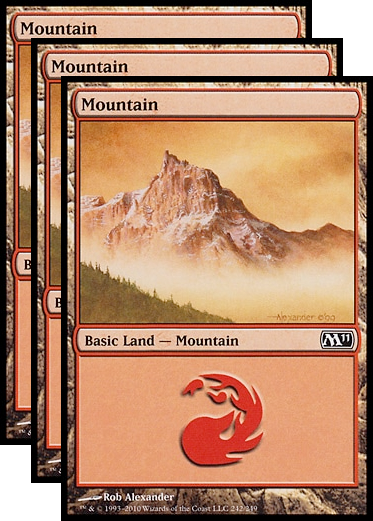
\includegraphics[width=0.2\textwidth]{picstcc/bf1.png}
    \vskip1ex
    $B_1$: O campo de batalha consiste apenas em 3 terrenos (Montanhas).

    \vspace{.1cm}

    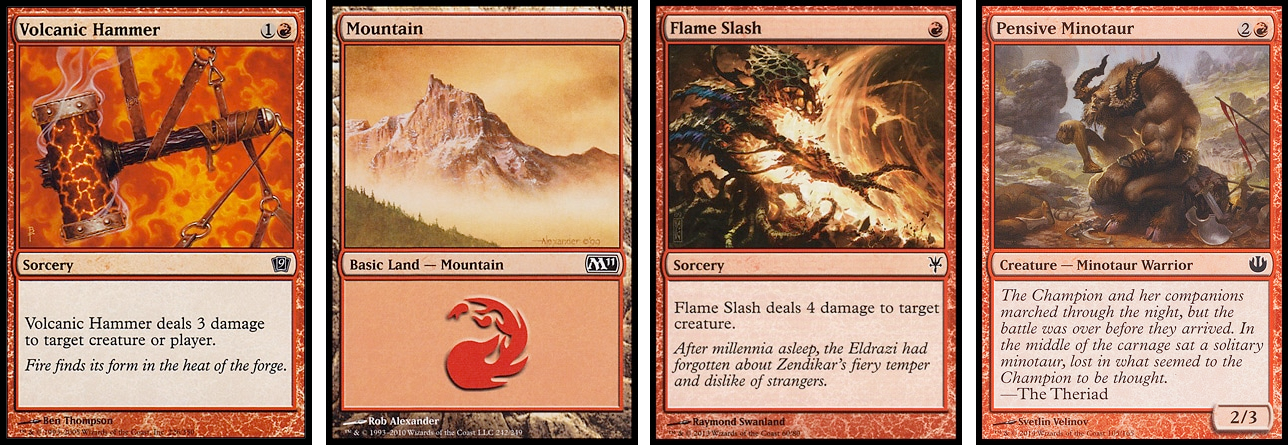
\includegraphics[width=0.9\textwidth]{picstcc/hand1.png}
    \vskip1ex
    $H$: A mão do agente consiste em um terreno (Montanha), um feitiço ``Volcanic Hammer'', um feitiço ``Flame Slash'' e uma criatura ``Pensive Minotaur''.

    \vskip1ex
    Dessa maneira, o conjunto de ações em $s_1$ pode ser definido a partir de $H$ e $B_1,B_2$:
    \begin{equation}
      A^P(s_1) := \begin{lrdcases}
                  Mountain \in Land, \\
                  PensiveMinotaur \in Creature(3), \\
                  VolcanicHammer(self) \in Sorcery(2, self), \\
                  VolcanicHammer(opponent) \in Sorcery(2, opponent), \\
                  Pass.
                  \end{lrdcases}
    \end{equation}
    Como não há criaturas em jogo, ``Flame Slash'' não tem alvos legais e não pode ser jogada. ``Volcanic Hammer'', por outro lado, admite ambos os jogadores como alvo válido, portanto pode ser jogada através de duas ações diferentes.
  \end{center}
\end{mdframed}

Suponhamos que o agente jogue a Montanha que tem na mão. Sendo assim, o estado $s_2$ é parecido com $s_1$.

\newpage

\textbf{Figura E.1.2:} estado $s_2$

\begin{mdframed}
    \begin{center}
    $s_2 = \left\{ v_1 = v_2 = 10, h_1 = 3, h_2 = 0, B_2 = G_1 = G_2 = \emptyset, B_1, H \right\}$
    \vskip1ex
    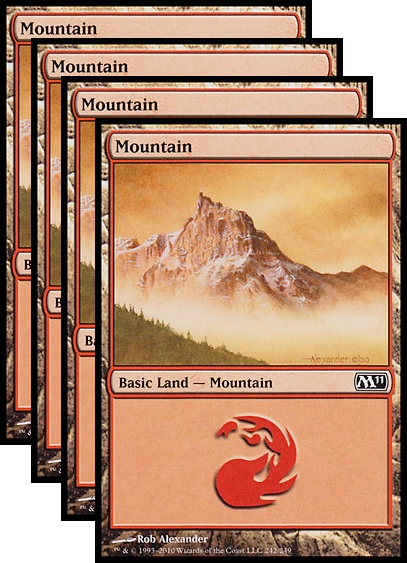
\includegraphics[width=0.2\textwidth]{picstcc/bf2.png}
    \vskip1ex
    $B_1$: O campo de batalha consiste apenas em 4 terrenos (Montanhas).

    \vspace{.1cm}

    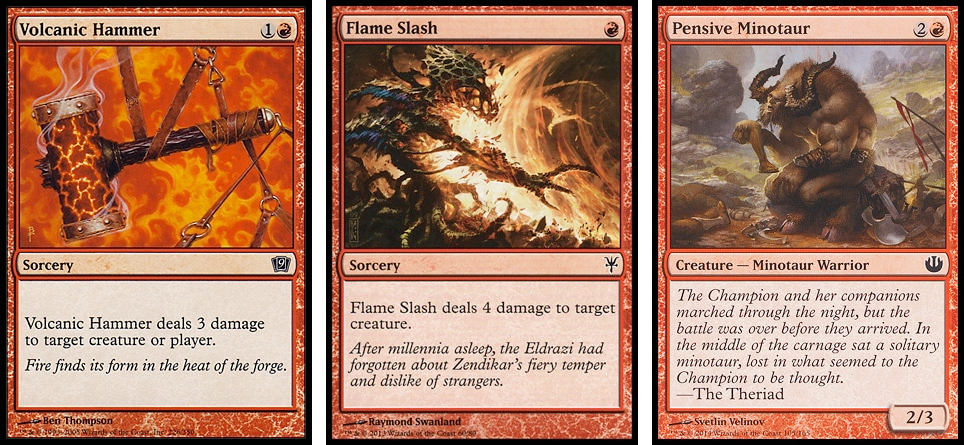
\includegraphics[width=0.9\textwidth]{picstcc/hand2.png}
    \vskip1ex
    $H$: A mão do agente consiste em um feitiço ``Volcanic Hammer'', um feitiço ``Flame Slash'' e uma criatura ``Pensive Minotaur''.

    \vskip1ex
    O conjunto de ações em $s_2$ é quase igual ao conjunto de ações em $s_1:$
    \begin{equation}
      A^P(s_2) := \begin{lrdcases}
                  PensiveMinotaur \in Creature(3), \\
                  VolcanicHammer(self) \in Sorcery(2, self), \\
                  VolcanicHammer(opponent) \in Sorcery(2, opponent), \\
                  Pass.
                  \end{lrdcases}
    \end{equation}
    ``Flame Slash'' ainda não pode ser jogada.
  \end{center}
\end{mdframed}

Agora, a ação escolhida em $s_2$ é jogar a carta ``Pensive Minotaur'', uma criatura sem efeitos. Para isso, é necessário virar 3 terrenos, alterando duplamente $B_1$.

\newpage
\textbf{Figura E.1.3:} estado $s_3$

\begin{mdframed}
    \begin{center}
    $s_3 = \left\{ v_1 = v_2 = 10, h_1 = 2, h_2 = 0, B_2 = G_1 = G_2 = \emptyset, B_1, H \right\}$
    \vskip1ex
    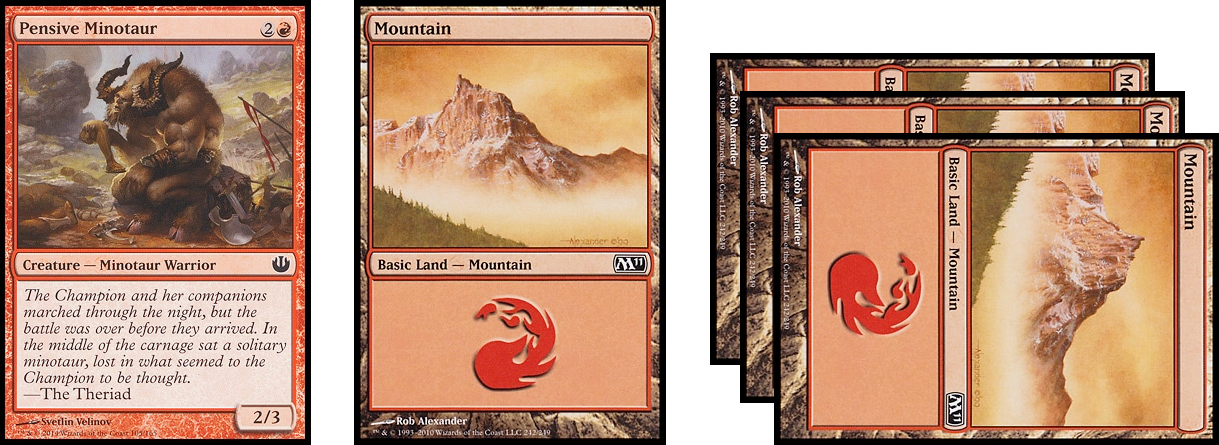
\includegraphics[width=0.6\textwidth]{picstcc/bf3.png}
    \vskip1ex
    $B_1$: Com ``Pensive Minotaur'' jogada, o campo de batalha agora contém ela, três montanhas viradas e uma montanha desvirada.

    \vspace{.1cm}

    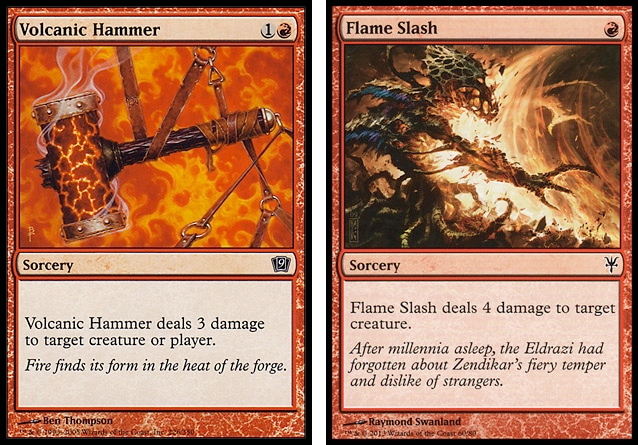
\includegraphics[width=0.7\textwidth]{picstcc/hand3.png}
    \vskip1ex
    $H$: A mão do agente consiste em um feitiço ``Volcanic Hammer'' e um feitiço ``Flame Slash''.

    \vskip1ex
    O conjunto de ações legais em $s_3$ muda radicalmente:
    \begin{equation}
      A^P(s_3) := \begin{lrdcases}
                  FlameSlash(Pensive Minotaur \in B_1) \in Sorcery(1, e \in B_1), \\
                  Pass.
                  \end{lrdcases}
    \end{equation}
    ``Flame Slash'' agora pode ser jogada.
  \end{center}
\end{mdframed}

Em $s_3$, como o agente tem apenas um terreno desvirado em jogo, jogar ``Volcanic Hammer'' em qualquer alvo passam a ser ações ilegais (pois são necessários dois terrenos para isso). Por outro lado, jogar ``Flame Slash'' passa a ser possível pois há uma criatura em campo (e a carta requer apenas uma Montanha). Apesar de parecer uma jogada péssima, para efeitos de exemplo suponhamos que esta ação seja tomada.

\newpage
\textbf{Figura E.1.4:} estado $s_4$

\begin{mdframed}
    \begin{center}
    $s_4 = \left\{ v_1 = v_2 = 10, h_1 = 2, h_2 = 0, B_2 = G_2 = \emptyset, B_1, H, G_1 \right\}$
    \vskip1ex
    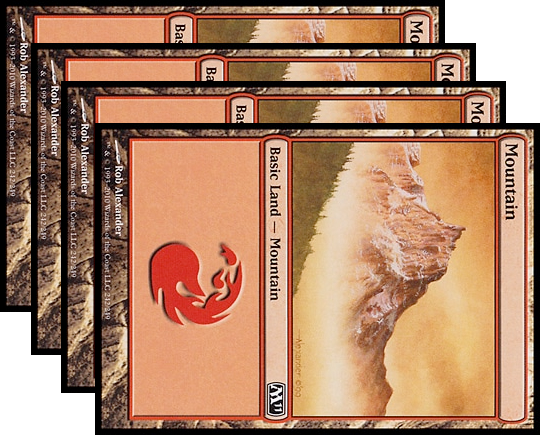
\includegraphics[width=0.33\textwidth]{picstcc/bf4.png}
    \vskip1ex
    $B_1$: ``Pensive Minotaur'' foi destruída, restam apenas as 3 Montanhas viradas usadas para jogá-la e a outra Montanha, virada, usada para jogar ``Flame Slash''.

    \vspace{.1cm}

    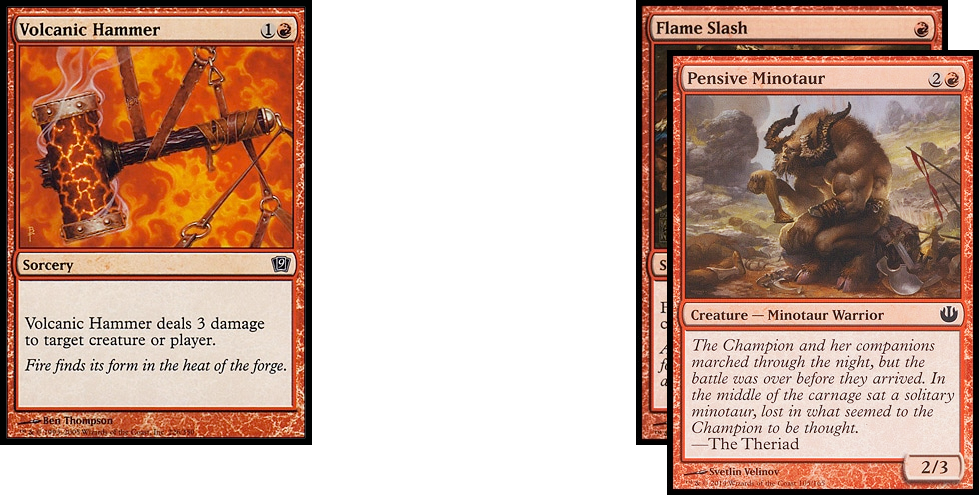
\includegraphics[width=0.6\textwidth]{picstcc/hand4.png}
    \vskip1ex
    $H$: A mão do agente consiste apenas em um feitiço ``Volcanic Hammer''. \\
    $G_1$: A pilha de descarte do agente, por sua vez, agora contém ambos o feitiço ``Flame Slash'' (quando um feitiço é usado, vai para a pilha de descarte) e a criatura ``Pensive Minotaur'' (destruída após o efeito de ``Flame Slash'' lhe causar dano maior ou igual à sua resistência).

    \vskip1ex
    A única ação legal em $s_4$ é passar para o final da fase:
    \begin{equation}
      A^P(s_4) := \begin{lrdcases}
                  Pass.
                  \end{lrdcases}
    \end{equation}
  \end{center}
\end{mdframed}

Apesar de ter um feitiço na mão, o agente não tem os recursos disponíveis para jogá-lo. Assim, a única ação legal é passar para a fase de combate, encerrando a primeira fase principal.


\newpage

\subsubsection{Combate}

O combate é bem diferente da fase principal, pois não há jogada de cartas ou informação incompleta: tudo acontece com as criaturas já no campo de batalha. Sua estrutura é a seguinte: o jogador ativo \textit{declara atacantes}, ou seja, escolhe quais das suas criaturas atacarão e, em seguida, seu oponente \textit{declara bloqueadores}, escolhendo quais das suas criaturas bloquearão cada criatura atacante. Após isso, cada criatura atacante causa dano igual a seu poder às criaturas que a bloquearam ou ao jogador defensor (caso não tenha sido bloqueada), e cada criatura bloqueadora causa dano igual a seu poder à criatura que bloqueou. Todo dano é causado ao mesmo tempo. Por fim, cada criatura com dano maior ou igual à sua resistência é destruída: sua carta sai do campo de batalha e passa para a pilha de descarte correspondente.\footnote{Nesta seção não trataremos das \textit{habilidades de criatura} relevantes para o combate, de maneira a simplificar as explicações. Trataremos melhor disso mais a frente.}

\vskip1ex

O conjunto $A^C_1$ de ações do jogador ativo no combate, portanto, é o conjunto de escolhas de todas as combinações de criaturas atacantes (incluindo nenhuma). Dado que o jogador deve escolher alguma combinação, \begin{equation}|A^C_1| = \sum\limits_{i = 0}^{N}\binom{N}{i} = 2^N,\end{equation} onde $N$ é o número de criaturas que podem atacar na mesa do jogador ativo.

\vskip1ex

O conjunto $A^C_2$ de ações do jogador não-ativo durante o combate, por sua vez, é o conjunto de escolhas de todas as combinações de criaturas bloqueadoras e aquelas que estas bloqueiam. Como cada criatura desvirada pode bloquear até uma criatura atacante, temos que \begin{equation} |A^C_2| = (N' + 1)^M \le (N + 1)^M, \end{equation} onde $N'$ é o número de criaturas atacantes e $M$ o número de criaturas aptas a bloquearem.

\vskip1ex

Assim como na fase principal, cada ação $a \in \left\{A^C_1, A^C_2\right\}$ no estado $s$ tomada tem probabilidade $P(s'| s, a) = 1$ para o estado $s'$ sucessor previsto pelas regras.

\vskip1ex

Nas próximas páginas demonstraremos por exemplos os estados e conjuntos de ações (de ambos jogadores) em uma fase de combate.

\newpage
\subsubsection{Exemplo - Combate}


Suponhamos um estado inicial $t_1$ da seguinte maneira (vamos suprimir as informações sobre mãos e baralhos pois estas são irrelevantes)

\vskip1ex

\textbf{Figura E.2.1:} estado $t_1$

\begin{mdframed}
    \begin{center}
    $t_1 = \left\{ v_1 = v_2 = 10, G_1 = G_2 = \emptyset, B_1, B_2 \right\}$
    \vskip1ex
    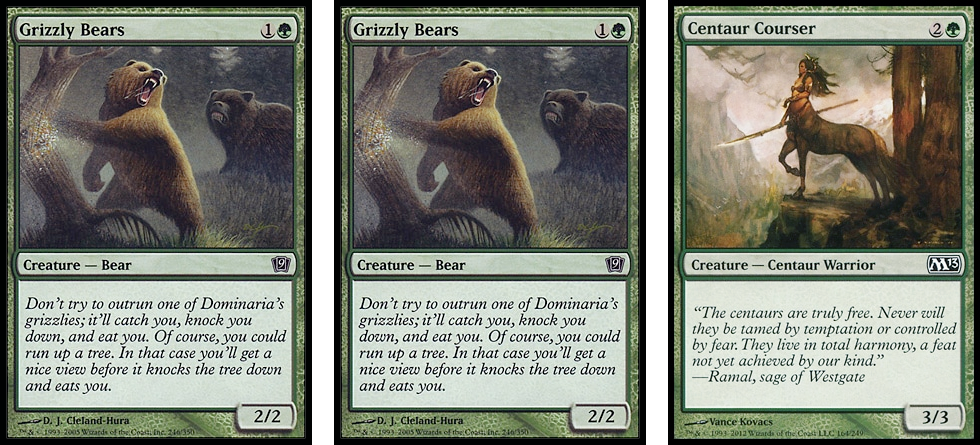
\includegraphics[width=0.5\textwidth]{picstcc/att1.png}
    \vskip1ex
    $B_1$: O jogador ativo tem três criaturas aptas a atacar em campo: dois ``Grizzly Bears'' e um ``Centaur Courser''. Assim, podemos obter o conjunto de ações legais $A^C_1$:

    \begin{equation}
      A^C_1(t_{1,1}) := \begin{lrdcases}
                  GrizzlyBears1, \\
                  GrizzlyBears2, \\
                  CentaurCourser, \\
                  \{ GrizzlyBears1, GrizzlyBears2\}, \\
                  \{ GrizzlyBears1, CentaurCourser \}, \\
                  \{GrizzlyBears2, CentaurCourser \}, \\
                  \{ GrizzlyBears1, GrizzlyBears2, CentaurCourser\}, \\
                  None.
                  \end{lrdcases}
    \end{equation}
    O jogador ativo pode declarar qualquer combinação (incluindo nenhuma) de criaturas como atacantes. Note que $N = 3$ e $|A^C_1| = 2^N = 8$.
  \end{center}
\end{mdframed}

Suponhamos que o jogador ativo escolheu a ação $\{GrizzlyBears2, CentaurCourser\}$ em $t_1$. Assim, o jogador declarou ambas suas criaturas como atacantes. Assim como com terrenos e geração de recursos, uma criatura atacante é virada quando declarada atacante (e precisa estar desvirada previamente para poder atacar). Assim, podemos obter o estado seguinte, $t_2$.

\newpage

\textbf{Figura E.2.2:} estado $t_2$

\begin{mdframed}
    \begin{center}
    $t_2 = \left\{ v_1 = v_2 = 10, G_1 = G_2 = \emptyset, B_1, B_2 \right\}$
    \vskip1ex
    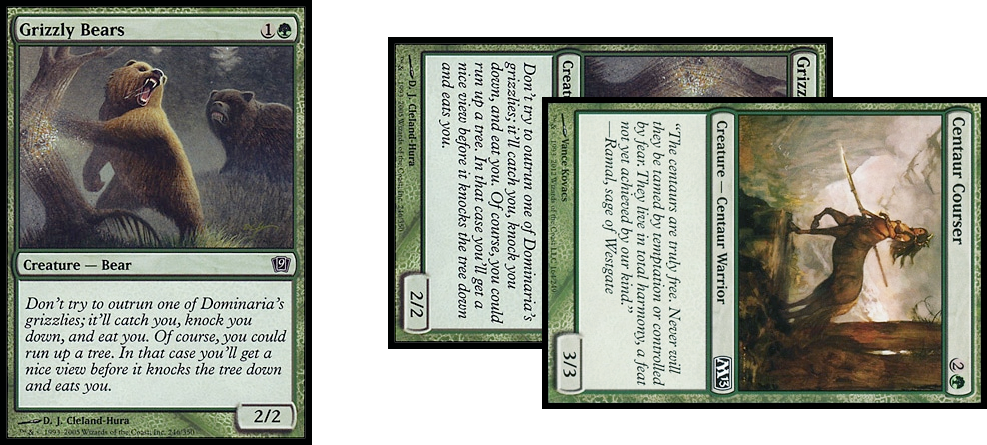
\includegraphics[width=0.5\textwidth]{picstcc/att2.png}
    \vskip1ex
    $B_1$: O jogador ativo tem um ``Grizzly Bears'' desvirado e um ``Grizzly Bears'' e um ``Centaur Courser'' virados, ambos atacando ($N' = 2$).

    \vskip1ex

    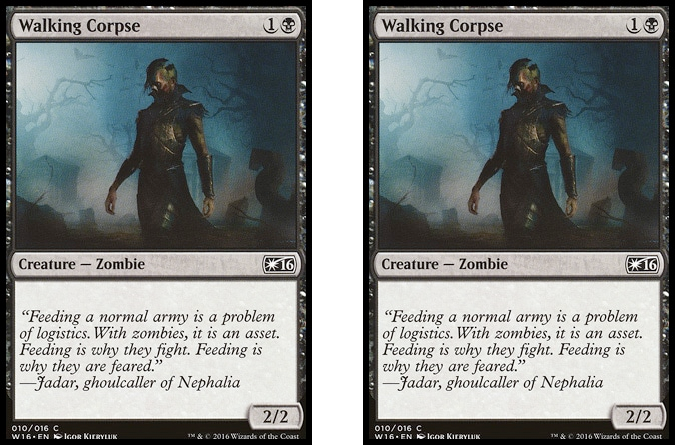
\includegraphics[width=0.4\textwidth]{picstcc/blk1.png}

    \vskip1ex
    $B_2$: O jogador defensor tem dois ``Walking Corpse'' desvirados (e aptos a bloquear). Portanto, as ações legais são todas as combinações de bloqueio das criaturas atacantes:

    \begin{equation}
      A^C_2(t_2) := \begin{lrdcases}
                  \{WalkingCorpse1 : None, WalkingCorpse2 : None\}, \\
                    \{WalkingCorpse1 : GrizzlyBears2, WalkingCorpse2 : None\}, \\
                  \{WalkingCorpse1 : CentaurCourser, WalkingCorpse2 : None\}, \\
                  \{WalkingCorpse1 : None, WalkingCorpse2 : GrizzlyBears2\}, \\
                  \{WalkingCorpse1 : None, WalkingCorpse2 : CentaurCourser\}, \\
                  \{WalkingCorpse1 : CentaurCourser, WalkingCorpse2 : GrizzlyBears2\}, \\
                  \{WalkingCorpse1 : GrizzlyBears2, WalkingCorpse2 : CentaurCourser\}, \\
                  \{WalkingCorpse1 : GrizzlyBears2, WalkingCorpse2 : GrizzlyBears2\}, \\
                  \{WalkingCorpse1 : CentaurCourser, WalkingCorpse2 : CentaurCourser\}.
                  \end{lrdcases}
    \end{equation}
    Assim, há $|A^C_2(t_2)| = (N' + 1)^M = (2 + 1)^2 = 9$ ações legais.
  \end{center}
\end{mdframed}

Assim, há alguns estados sucessores possíveis. Vamos examinar algumas configurações de bloqueio distintas\footnote{Algumas ações são essencialmente a mesma, pois os dois ``Walking Corpse'' não têm diferenças. Como, nas regras do jogo, são considerados objetos diferentes, estamos distinguindo-os para manter a consistência.} e seus respectivos estados sucessores.

\newpage

\textbf{Figura E.2.3:} estado $t_3$

\begin{mdframed}

    Suponhamos que a ação escolhida pelo agente tenha sido \[\{WalkingCorpse1 : GrizzlyBears2, WalkingCorpse2 : None\},\] ou seja, bloquear ``Grizzly Bears'' com um ``Walking Corpse'' e não bloquear ``Centaur Courser''.

    \begin{center}
    \vskip1ex
    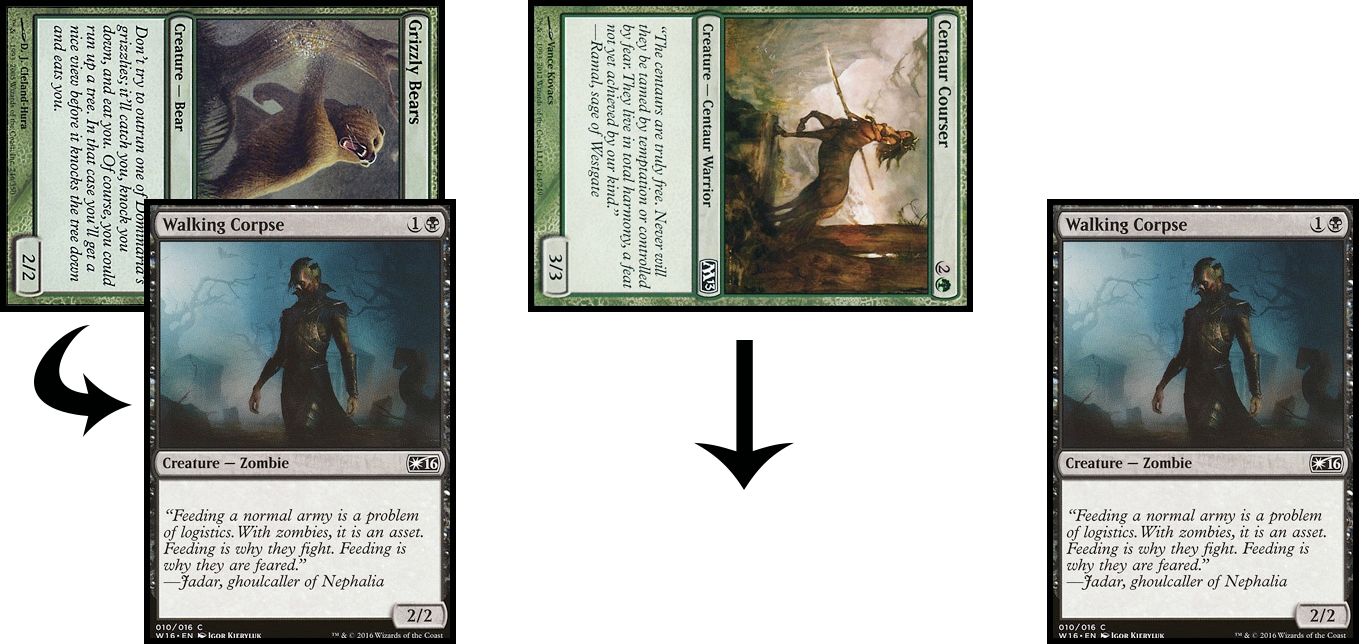
\includegraphics[width=0.9\textwidth]{picstcc/blk2.png}
    \vskip1ex
    Esta é a representação da ``resolução do combate'' pré-$t_3$. O estado $t_3$, portanto, refletirá as consequências das ações escolhidas. Podemos listá-las:
    \begin{itemize}
      \item ``Grizzly Bears'' causou um número igual a seu poder (2) de dano ao ``Walking Corpse'' que o bloqueou.
      \item ``Walking Corpse'' causou um número igual a seu poder (2) de dano ao ``Grizzly Bears'' bloqueado.
      \item ``Centaur Courser'' não foi bloqueado, causando um número igual a seu poder (3) de dano ao jogador defensor.
    \end{itemize}
    \end{center}

    Assim, ambos ``Grizzly Bear'' e ``Walking Corpse'' são destruídos (pois receberam dano maior ou igual às suas resistências) e temos o seguinte estado $t_3$:

    \[t_3 = \begin{lrdcases}
           v_1 = 10, v_2 = 10 - 3 = 7, \\
           G_1 = \{ GrizzlyBears2 \}, G_2 = \{ WalkingCorpse1 \}, \\
           B_1 = \{ GrizzlyBears1(u), CentaurCourser(t)\}, \\
           B_2 = \{ WalkingCorpse2(u) \}.
           \end{lrdcases}\]
    O parâmetro $u$ de uma permanente significa que ela está desvirada, enquanto $t$ significa que está virada.
\end{mdframed}

Em $t_3$, ambos os jogadores tem uma criatura (essencialmente igual, pois têm os mesmos atributos) a menos em relaçnao a $t_2$, mas o jogador defensor perdeu pontos de vida.

\pagebreak

\textbf{Figura E.2.4:} estado $t'_3$

\begin{mdframed}

    Suponhamos, por outro lado, que a ação escolhida pelo agente tenha sido \[\{WalkingCorpse1 : GrizzlyBears2, WalkingCorpse2 : CentaurCourser\},\] ou seja, bloquear ``Grizzly Bears'' com um ``Walking Corpse'' e ``Centaur Courser'' com o outro.

    \begin{center}
    \vskip1ex
    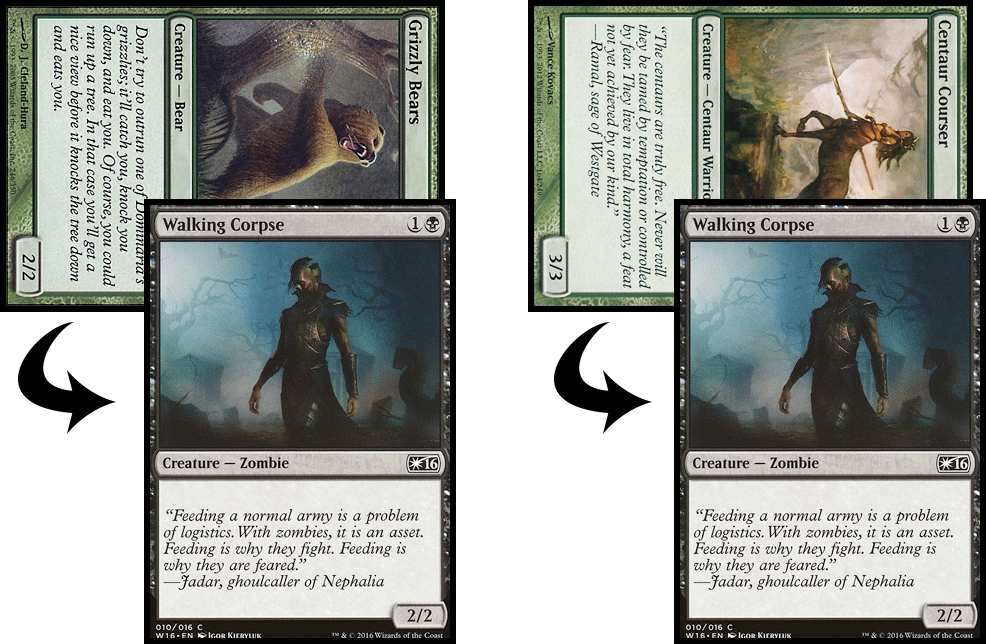
\includegraphics[width=0.9\textwidth]{picstcc/blk3.png}
    \vskip1ex
    Representação do combate. O estado $t'_3$ refletirá as seguintes consequências:
    \begin{itemize}
      \item ``Grizzly Bears'' causou um número igual a seu poder (2) de dano ao ``Walking Corpse'' que o bloqueou.
      \item ``Walking Corpse'' causou um número igual a seu poder (2) de dano ao ``Grizzly Bears'' bloqueado.
      \item ``Centaur Courser'' causou um número igual a seu poder (3) de dano ao ``Walking Corpse'' que o bloqueou.
      \item ``Walking Corpse'' causou um número igual a seu poder (2) de dano ao ``Centaur Corser'' bloqueado.
    \end{itemize}
    \end{center}

    Assim, ``Grizzly Bears'' e os dois ``Walking Corpse'' são destruídos (pois receberam dano maior ou igual às suas resistências) e temos o seguinte estado $t'_3$:

    \[t'_3 = \begin{lrdcases}
           v_1 = 10, v_2 = 10, \\
           G_1 = \{ GrizzlyBears2 \}, G_2 = \{ WalkingCorpse1, WalkingCorpse2 \}, \\
           B_1 = \{ GrizzlyBears1(u), CentaurCourser(t)\}, \\
           B_2 = \emptyset.
           \end{lrdcases}\]
\end{mdframed}

Em $t'_3$, o total de pontos de vida não foi alterado, mas a balança do combate também parece negativa para o jogador defensor, que acabou sem criaturas na mesa. Note que o dano causado a ``Centaur Courser'' não foi suficiente para destruí-lo\footnote{De acordo com as regras, o dano causado a uma criatura permanece até o final do turno. Se, porventura, algum dano fosse causado a ``Centaur Courser'' na segunda fase principal, a criatura também seria destruída.}.

\textbf{Figura E.2.5:} estado $t''_3$

\begin{mdframed}

    Por fim, suponhamos que a ação escolhida pelo agente tenha sido \[\{WalkingCorpse1 : CentaurCourser, WalkingCorpse2 : CentaurCourser\},\] ou seja, bloquear ``Centaur Courser'' com os dois ``Walking Corpse''.

    \begin{center}
    \vskip1ex
    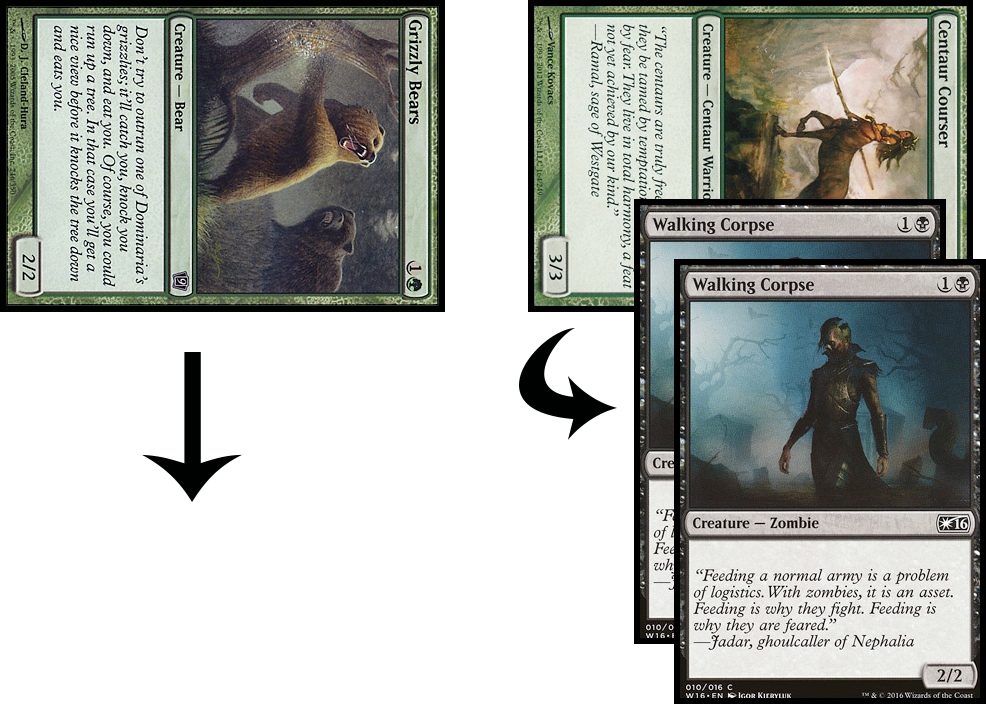
\includegraphics[width=0.9\textwidth]{picstcc/blk4.png}
    \vskip1ex
    Representação do combate. O estado $t''_3$ refletirá as seguintes consequências:
    \begin{itemize}
      \item ``Centaur Courser'' causou um número igual a seu poder (3) de dano aos ``Walking Corpse'' que o bloquearam.
      \item Os dois ``Walking Corpse'' causaram um número igual a seu poder (2 + 2) de dano ao ``Centaur Courser'' bloqueado.
      \item ``Grizzly Bears'' causou um número igual a seu poder (2) de dano ao ``Walking Corpse'' que o bloqueou.
      \item ``Walking Corpse'' causou um número igual a seu poder (2) de dano ao ``Centaur Corser'' bloqueado.
    \end{itemize}
    \end{center}

    Como ``Centaur Courser'' recebeu dano total (4) maior ou igual a sua resistência, foi destruído. Por outro lado, ``Centaur Courser'' causou no total (3) dano suficiente para destruir apenas um ``Walking Corpse'' (e danificar em 1 o outro). O estado $t''_3$, portanto, é configurado assim:

    \[t''_3 = \begin{lrdcases}
           v_1 = 10, v_2 = 10 - 2 = 8, \\
           G_1 = \{ CentaurCourser \}, G_2 = \{ WalkingCorpse1 \}, \\
           B_1 = \{ GrizzlyBears1(u), GrizzlyBears2(t)\}, \\
           B_2 = \{ WalkingCorpse2 \}.
           \end{lrdcases}\]
\end{mdframed}

Podemos perceber que, para o jogador defensor, a situação é estritamente melhor em $t''_3$ do que em $t_3$, pois $v_2(t''_3) > v_2(t_3)$ e, apesar de ter perdido a mesma criatura em ambos os casos, em $t''_3$ o jogador defensor conseguiu destruir uma criatura maior do oponente no processo. Além disso, apesar de não ser estritamente pior, pois não houve perda de vida, a situação em $t'_3$ parece também pior para o jogador defensor do que em $t''_3$, já que acabou perdendo suas duas criaturas.



\item $R$ : Por fim, precisamos definir as recompensas por sair de cada estado. Uma boa definição inicial leva em conta os pontos de vida do agente e do oponente, assim como as ``presenças de campo'', termo vago que dá a ideia de progresso no jogo. Escolhemos medir a ``presença de campo'' de cada jogador com o dano que suas criaturas podem causar, ou seja, a soma do poder de todas as suas criaturas. Assim, dados pontos de vida $v_1, v_2$ respectivos do agente e seu oponente e seus conjuntos de permanentes $B_1, B_2$, temos

\begin{equation}
  R(s'|s, a) = \begin{cases}
              -\gamma, &\textrm{ caso $v_1 \le 0$,} \\
              +\gamma, &\textrm{ caso $v_2 \le 0$,} \\
              v_1 + v_2 + \sum\limits_{e \in B_1} pow(e) - \sum\limits_{e \in B_2} pow(e), &\textrm{ cc.}
            \end{cases},
\end{equation}
onde $\gamma$ deve ser uma recompensa para o agente suficientemente alta para incentivar a derrota do oponente e evitar a própria. A função $pow(e)$ retorna o poder da permanente $e$.

\vskip1ex

Podemos, então, calcular as recompensas de acordo com $R$ por sair dos estados nos exemplos demonstrados por meio das ações escolhidas:

\begin{itemize}
  \item $R(s_2 | s_1, Mountain) = v_1 - v_2 = 10 - 10 = 0.$
  \item $R(s_3 | s_2, PensiveMinotaur(3)) = v_1 - v_2 + pow(PensiveMinotaur) = 0 + 2 = 2.$
  \item $R(s_4 | s_3, FlameSlash(1, PensiveMinotaur)) = v_1 - v_2 + 0 = 0.$
\end{itemize}

Vamos examinar agora as recompensas no exemplo de combate tomando como agente o jogador defensor (portanto, as recompensas são contrárias - $v_2$ e $B_2$ são relativos aos agentes):

\begin{itemize}
  \item $R(t_3 | t_2, \{WalkingCorpse1 : GrizzlyBears2, WalkingCorpse2 : None\}) = v_2 - v_1 + \sum\limits_e(pow(e) : e \in B_2) - \sum\limits_e(pow(e) : e \in B_1) = 7 - 10 + 2 - 5 = -6.$
  \item $R(t'_3| t_2, \{WalkingCorpse1 : GrizzlyBears2, WalkingCorpse2 : CentaurCourser\}) = 10 - 10 + 0 - 3 = -3.$
  \item $R(t''_3| t_2, \{WalkingCorpse1 : CentaurCourser, WalkingCorpse2 : CentaurCourser\}) = 8 - 10 + 2 - 2 = -2.$
\end{itemize}
Estas recompensas refletem a noção de que o estado $t''_3$ é mais desejável para o jogador defensor do que os outros.

\end{itemize}

\newpage

\subsection{Estratégias e algoritmos}

Um turno inteiro de \textit{Magic} tem, como mostrado, muitos estados possíveis. Para determinar
em primeira instância as ações de um turno, é possível realizar uma busca local exaustiva dentre todas as
possibilidades. Tomando o turno atual como escopo, podemos definir uma recompensa para qualquer
estado final (que sempre será após a ação \textit{Pass} na segunda Fase Principal), que assumirá o valor 0
nos outros casos (como examinaremos todas as possibilidades, faz sentido que a recompensa só seja avaliada
após a aplicação de toda a sequência). Esta busca, analogamente à divisão do turno, tem três partes:

\subsubsection{Busca Local - Fase Principal}

Uma busca local em um problema de Inteligência Artificial consiste, resumidamente, em construir uma árvore
de estados através de uma função $Vizinhos(s, a)$ que retorna os possíveis estados-sucessores de um estado $s$ após
a aplicação de uma ação $a$ (dadas as restrições já impostas no problema, sabemos que a função $Vizinhos(s, a)$ sempre
retornará apenas um estado). Assim, o agente pode prever o resultado da aplicação de uma sequência de ações e explorar o espaço de estados até encontrar o que deseja. Os dois algoritmos básicos de busca local são a busca em \textbf{profundidade} e busca
em \textbf{largura}.

\vskip1ex
Na busca em profundidade, usa-se uma estrutura de pilha:toda vez que uma ação exploratória é tomada, o
estado sucessor é empilhado, geralmente havendo \textit{backtracking} quando um estado admite estados sucessores diferentes. Por exemplo,
suponhamos que um agente deve resolver um labirinto. Ao efetuar uma busca em profundidade, empilhará estados explorados até encontrar
um estado sem sucessores. Caso este estado seja a saída do labirinto, o problema é resolvido; caso contrário, o agente retira estados
da pilha até encontrar o último estado com sucessores não-explorados do caminho -- e, a partir dele, continua a busca.

\vskip1ex
Por outro lado, a busca em largura utiliza uma fila: dado um estado examinado $s$, todos os seus sucessores
não-visitados são inseridos na fila, de modo a serem explorados posteriormente. A busca em largura permite comparar mais naturalmente
custos (ou, no nosso caso, recompensas) associados a estados finais e/ou caminhos, sendo mais adequada para examinar exaustivamente
todos os estados -- justamente o que queremos. Sendo assim, é um algoritmo adequado para decidir a sequência de ações com maior
recompensa em um turno.

\subsubsection{Minimax - Combate}

A etapa de combate consiste em três decisões, como explicado na seção \ref{gamestructure}:

\begin{enumerate}
  \item \textbf{Jogador ativo} declara criaturas atacantes.
  \item \textbf{Jogador defensor} declara criaturas bloqueadoras.
  \item \textbf{Jogador ativo} escolhe a ordem da atribuição do dano (caso haja mais de uma criatura bloqueadora
  para alguma criatura atacante).
\end{enumerate}

Dada a natureza alternada das ações, escolhemos utilizar a regra de decisão \textit{Minimax} (de minimização-maximização, também podendo ser escrita como \textit{Maximin}) para submeter uma ação. O \textit{Minimax}, intuitivamente, busca minimizar a maior perda futura possível ao realizar uma ação. Para isso, supõe-se que, dada uma ação $a$ escolhida pelo agente em questão, seu adversário escolherá racionalmente uma ação $a'$ que maximize a perda do agente. Assim, o agente consegue realizar uma busca dentre todas as suas ações e determinar a mais ``segura'', ou seja, que minimiza a perda máxima após a escolha da ação $a_1$ por seu adversário. Podemos definir a seguinte função-valor para um estado $s$ e seu sucessor $s'$ lembrando que a ação em $s$ é escolhida pelo agente e, em $s'$, por seu adversário:

\begin{equation*}
  MM_s = \max\limits_{a \in A(s)}\left(\min\limits_{a' \in A(s')}\left(MM_{s'}\right)\right)
\end{equation*}

Como a função é definida recursivamente, é necessário definir um critério de parada e seu comportamento neste caso. O usual para o \textit{Minimax} é definir uma profundidade máxima $n$ e, de alguma maneira, avaliar os ganhos (ou perdas) de todos os estados possíveis nesta profundidade (que se propagarão até a ``superfície'' -- a primeira decisão). No caso do combate, como temos 3 decisões, podemos definir sem preocupações a profundidade $n = 2$ e os ganhos com uma função-recompensa igual à da busca em largura da primeira Fase Principal (afinal, os objetivos são os mesmos). Quando o agente é o jogador defensor, sua decisão (ou seja, como declarar as criaturas bloqueadoras) levará em conta apenas a ordem que o jogador ativo escolherá, depois, a atribuição de dano, logo, neste caso, a profundidade da árvore \textit{Minimax} é 1.

\subsubsection{Combinando estratégias}

Para definir a recompensa no final de um turno, então, devemos combinar ambas buscas. Isso é feito naturalmente ao expandirmos a busca em largura em uma fase principal para o turno todo, incorporando o estado pós-combate determinado pela busca \textit{Minimax}. Como o combate é influenciado pelas ações tomadas no primeiro turno, cada sequência de ações terá uma previsão de combate própria. O estado pós-combate é o começo da segunda Fase Principal e, partir dele, podemos continuar a busca em largura até o final do turno, quando avaliaremos a recompensa associada a cada sequência (total) de ações.

\vskip1ex

Como o agente pode prever incorretamente as escolhas de bloqueio de seu oponente (caso este não realize um \textit{Minimax} ou avalie recompensas de um modo diferente, por exemplo), é possível que o estado no início da segunda Fase Principal seja diferente do previsto. Assim, a busca na segunda Fase Principal deve ser refeita para encontrar a ``nova'' melhor recompensa total do turno. Como isso ocorre quando o jogador defensor não escolhe sua ``melhor'' (segundo os critérios do agente) configuração de bloqueio, é de certa forma positivo para o agente, pois lhe dá a chance de encontrar sequência de ações com uma recompensa maior para o turno.

\subsection{Detalhes da Implementação}

A classe \texttt{SearchAgent} é derivada de \texttt{MulliganAgent} para que decida o \textit{mulligan} baseando-se nas políticas encontradas pela iteração de valor. Iremos examinar seus métodos principais a seguir.

\begin{Verbatim}[commandchars=\\\{\}]
 \PY{l+m+mi}{1} \PY{k}{def} \PY{n+nf}{breadthFirstSearch}\PY{p}{(}\PY{n+nb+bp}{self}\PY{p}{,} \PY{n}{startState}\PY{p}{)}\PY{p}{:}
 \PY{l+m+mi}{2}     \PY{n}{q} \PY{o}{=} \PY{n}{queue}\PY{o}{.}\PY{n}{Queue}\PY{p}{(}\PY{p}{)}
 \PY{l+m+mi}{3}     \PY{n}{q}\PY{o}{.}\PY{n}{put}\PY{p}{(}\PY{n}{startState}\PY{p}{)}
 \PY{l+m+mi}{4}     \PY{n}{maxReward} \PY{o}{=} \PY{o}{\PYZhy{}}\PY{l+m+mi}{200}
 \PY{l+m+mi}{5}     \PY{n}{actionPath} \PY{o}{=} \PY{p}{[}\PY{p}{]}

 \PY{l+m+mi}{6}     \PY{k}{while} \PY{o+ow}{not} \PY{n}{q}\PY{o}{.}\PY{n}{empty}\PY{p}{(}\PY{p}{)}\PY{p}{:}
 \PY{l+m+mi}{7}         \PY{n}{state} \PY{o}{=} \PY{n}{q}\PY{o}{.}\PY{n}{get}\PY{p}{(}\PY{p}{)}

 \PY{l+m+mi}{8}         \PY{k}{if} \PY{n}{state}\PY{o}{.}\PY{n}{isTerminal}\PY{p}{(}\PY{p}{)}\PY{p}{:}
 \PY{l+m+mi}{9}             \PY{n}{reward} \PY{o}{=} \PY{n}{state}\PY{o}{.}\PY{n}{getReward}\PY{p}{(}\PY{p}{)}
\PY{l+m+mi}{10}             \PY{k}{if} \PY{n}{reward} \PY{o}{\PYZgt{}}\PY{o}{=} \PY{n}{maxReward}\PY{p}{:}
\PY{l+m+mi}{11}                 \PY{n}{maxReward} \PY{o}{=} \PY{n}{reward}
\PY{l+m+mi}{12}                 \PY{n}{actionPath} \PY{o}{=} \PY{n}{state}\PY{o}{.}\PY{n}{getPath}\PY{p}{(}\PY{p}{)}

\PY{l+m+mi}{13}         \PY{k}{else}\PY{p}{:}
\PY{l+m+mi}{14}             \PY{k}{for} \PY{n}{s} \PY{o+ow}{in} \PY{n+nb+bp}{self}\PY{o}{.}\PY{n}{getChildren}\PY{p}{(}\PY{n}{state}\PY{p}{)}\PY{p}{:}
\PY{l+m+mi}{15}                 \PY{n}{q}\PY{o}{.}\PY{n}{put}\PY{p}{(}\PY{n}{s}\PY{p}{)}

\PY{l+m+mi}{16}     \PY{k}{return} \PY{n}{actionPath}
\end{Verbatim}


A partir de um estado inicial \texttt{startState}, este método inicializa a fila de estados e, enquanto a fila não está vazia, repete a seguinte rotina: 8-12 checa se o estado é terminal, caso seja compara sua recompensa com a maior recompensa encontrada; caso não seja, nas linhas 13-15 coloca seus sucessores na fila. O método é simples, mas faz uso de outra classe: \texttt{State}, que define os estados.

\begin{Verbatim}[commandchars=\\\{\}]
\PY{k}{class} \PY{n+nc}{State}\PY{p}{:}
    \PY{k}{def} \PY{n+nf+fm}{\PYZus{}\PYZus{}init\PYZus{}\PYZus{}}\PY{p}{(}\PY{n+nb+bp}{self}\PY{p}{,} \PY{n}{game}\PY{p}{,} \PY{n}{phase}\PY{p}{,} \PY{n}{actionPath}\PY{p}{)}\PY{p}{:} \PY{o}{.}\PY{o}{.}\PY{o}{.}
    \PY{k}{def} \PY{n+nf}{isTerminal}\PY{p}{(}\PY{n+nb+bp}{self}\PY{p}{)}\PY{p}{:}  \PY{o}{.}\PY{o}{.}\PY{o}{.}
    \PY{k}{def} \PY{n+nf}{getReward}\PY{p}{(}\PY{n+nb+bp}{self}\PY{p}{)}\PY{p}{:}   \PY{o}{.}\PY{o}{.}\PY{o}{.}
    \PY{o}{.} \PY{o}{.} \PY{o}{.}
\end{Verbatim}


O construtor da classe recebe como parâmetro o jogo, a fase atual de jogo (em uma \textit{string}) e o caminho de ações escolhido para chegar nele. A partir das informações do jogo é possível extrair os atributos do estado relevantes para a determinação da recompensa. O método \texttt{isTerminal()} retorna \texttt{True} ou \texttt{False} dependendo se o estado é terminal ou não. Isso é determinado caso a fase seja \texttt{'End'} (sucessora de um estado na segunda Fase Principal) ou algum dos jogadores tenha perdido o jogo (o que pode acontecer a qualquer fase). O método \texttt{getChildren()} (equivalente à função $Vizinhos(s, a)$ aplicada a todas as ações possíveis de um estado) é chamado pelo método homônimo na classe \texttt{SearchAgent} (que simplesmente chama \texttt{state.getchildren()} quando a fase é alguma das duas fases principais ou o método \texttt{combatMinimax()}, quando a fase do estado atual é \texttt{'Combate'}).

\begin{Verbatim}[commandchars=\\\{\}]
\PY{k}{def} \PY{n+nf}{getChildren}\PY{p}{(}\PY{n+nb+bp}{self}\PY{p}{)}\PY{p}{:}
    \PY{n}{children} \PY{o}{=} \PY{p}{[}\PY{p}{]}
    \PY{k}{if} \PY{n+nb+bp}{self}\PY{o}{.}\PY{n}{phase} \PY{o}{==} \PY{l+s+s1}{\PYZsq{}}\PY{l+s+s1}{First Main}\PY{l+s+s1}{\PYZsq{}} \PY{o+ow}{or} \PY{n+nb+bp}{self}\PY{o}{.}\PY{n}{phase} \PY{o}{==} \PY{l+s+s1}{\PYZsq{}}\PY{l+s+s1}{Second Main}\PY{l+s+s1}{\PYZsq{}}\PY{p}{:}
        \PY{k}{for} \PY{n}{action} \PY{o+ow}{in} \PY{n+nb+bp}{self}\PY{o}{.}\PY{n}{game}\PY{o}{.}\PY{n}{getMainActions}\PY{p}{(}\PY{p}{)}\PY{p}{:}
            \PY{n}{game} \PY{o}{=} \PY{n+nb+bp}{self}\PY{o}{.}\PY{n}{game}
            \PY{n}{nextPhase} \PY{o}{=} \PY{n+nb+bp}{self}\PY{o}{.}\PY{n}{phase}
            \PY{k}{if} \PY{n}{action}\PY{p}{[}\PY{l+m+mi}{0}\PY{p}{]} \PY{o}{!=} \PY{l+s+s1}{\PYZsq{}}\PY{l+s+s1}{Pass}\PY{l+s+s1}{\PYZsq{}}\PY{p}{:}
                \PY{n}{game} \PY{o}{=} \PY{n}{c}\PY{o}{.}\PY{n}{deepcopy}\PY{p}{(}\PY{n+nb+bp}{self}\PY{o}{.}\PY{n}{game}\PY{p}{)}
                \PY{n}{game}\PY{o}{.}\PY{n}{play}\PY{p}{(}\PY{n}{action}\PY{p}{)}
                \PY{n}{game}\PY{o}{.}\PY{n}{checkSBA}\PY{p}{(}\PY{p}{)}
            \PY{k}{elif} \PY{n+nb+bp}{self}\PY{o}{.}\PY{n}{phase} \PY{o}{==} \PY{l+s+s1}{\PYZsq{}}\PY{l+s+s1}{First Main}\PY{l+s+s1}{\PYZsq{}}\PY{p}{:}
                \PY{n}{nextPhase} \PY{o}{=} \PY{l+s+s1}{\PYZsq{}}\PY{l+s+s1}{Combat}\PY{l+s+s1}{\PYZsq{}}
            \PY{k}{elif} \PY{n+nb+bp}{self}\PY{o}{.}\PY{n}{phase} \PY{o}{==} \PY{l+s+s1}{\PYZsq{}}\PY{l+s+s1}{Second Main}\PY{l+s+s1}{\PYZsq{}}\PY{p}{:}
                \PY{n}{nextPhase} \PY{o}{=} \PY{l+s+s1}{\PYZsq{}}\PY{l+s+s1}{End}\PY{l+s+s1}{\PYZsq{}}
            \PY{n}{children}\PY{o}{.}\PY{n}{append}\PY{p}{(}\PY{n}{State}\PY{p}{(}\PY{n}{game}\PY{p}{,} \PY{n}{nextPhase}\PY{p}{,} \PY{n+nb+bp}{self}\PY{o}{.}\PY{n}{actionPath} \PY{o}{+} \PY{p}{[}\PY{n}{action}\PY{p}{]}\PY{p}{)}\PY{p}{)}
    \PY{k}{else}\PY{p}{:}
        \PY{n}{children} \PY{o}{=} \PY{n+nb+bp}{self}\PY{o}{.}\PY{n}{combatMinimax}\PY{p}{(}\PY{p}{)}
    \PY{k}{return} \PY{n}{children}
\end{Verbatim}


O método \texttt{getChildren()} no estado encontra todas as ações legais de uma Fase Principal e, para cada uma, faz uma \textbf{cópia profunda} do jogo. Por fim,  ``dentro da cópia'' (pois não queremos alterar o jogo ``real''), joga a ação. A partir dos resultados da ação, um novo estado é criado (com a cópia do jogo como referência). O método retorna a lista de todos os estados criados desta maneira. Ainda, o método \texttt{combatMinimax()} da classe do agente funciona com a mesma ideia: explorar a árvore \textit{Minimax} criando cópias do jogo. Como o método é mais complexo (e chama 2 métodos parecidos), vamos simplificá-lo em pseudocódigo.

\begin{algorithm}
\caption*{\textbf{Minimax para Combate} (estado $s$):}
\begin{algorithmic}
  \STATE $a_{max} \gets \emptyset$
  \STATE recompensa máxima $r^1_{max} \gets -\infty$
  \STATE configurações de ataque $A^C_1 \gets A(s)$
  \STATE \textbf{para cada} ação de ataque $a \in A^C_1:$
    \STATE \ind $s' \gets $ cópia($s$)
    \STATE \ind $s' \gets $ aplica ação($s', a$)
    \STATE \ind recompensa mínima $r^2_{min} \gets +\infty$
    \STATE \ind configurações de bloqueio $A^C_2 \gets A(s')$
    \STATE
    \STATE \ind \textbf{para cada} ação de bloqueio $b \in A^C_2:$
      \STATE \ind \ind $s'' \gets $ cópia($s'$)
      \STATE \ind \ind $s'' \gets $ aplica ação($s'', b$)
      \STATE \ind \ind recompensa máxima $r^3_{max} \gets -\infty$
      \STATE \ind \ind ordenações de bloqueio $A^C_3 \gets A(s'')$
      \STATE
      \STATE \ind \ind \textbf{para cada} ação de ordenação $c \in A^C_3:$
        \STATE \ind \ind \ind $s'''\gets $ cópia($s''$)
        \STATE \ind \ind \ind $s'''\gets $ aplica ação($s''', c$)
        \STATE \ind \ind \ind $r \gets $ recompensa($s'''$)
        \STATE \ind \ind \ind \textbf{se } $r > r^3_{max}$ \textbf{então: }
        \STATE \ind \ind \ind \ind $r^3_{max} \gets r$
      \STATE
      \STATE \ind \ind \textbf{se } $r^3_{max} < r^2_{min}$ \textbf{então: }
      \STATE \ind \ind \ind $r^2_{min} \gets r^3_{max}$
      \STATE \ind \ind \ind $b_{min} \gets b$
    \STATE
    \STATE \ind \textbf{se } $r^2_{min} > r^1_{max}$ \textbf{então: }
    \STATE \ind \ind $r^1_{max} \gets r^2_{min}$
    \STATE \ind \ind $a_{max} \gets a$
    \STATE
    \STATE \textbf{devolva } $a_{max}$
\end{algorithmic}
\end{algorithm}


\chapter{Resultados}
Neste capítulo gostaríamos de analisar os resultados obtidos aplicando os algoritmos descritos no
capítulo anterior.

\section{Mulligan}
A política encontrada com a iteração de valor faz bastante sentido se levarmos em consideração a
simplificação de limitar a informação das cartas na mão ao fato dela ser terreno ou não. Uma
maneira de deixar a modelagem mais real seria levar em consideração o custo de mana dos cards
não-terreno. Isso aumentaria enormemente a quantidade de estados possíveis (supondo que as cartas
não-terreno do deck tenham custo de mana entre $1$ e $5$, uma mão com duas cartas teria
$\sum\limits_{i=1}^{6}i = 21$ representações possíveis de estados ao invés de $3$, como acontece
com a modelagem que escolhemos), mas essa modelagem ainda estaria desconsiderando informações
relevantes na decisão do mulligan, como por exemplo se as cartas na mão inicial se encaixam na
estratégia definida pelo jogador para combater o deck adversário. De uma maneira geral, estamos
satisfeitos com os resultados obtidos, uma vez que o agente consegue mitigar a aleatoriedade
tomando decisões que aumentam suas chances de ter um jogo justo.

\section{O Jogo}
Após rodar os experimentos várias vezes e analisar os resultados, conseguimos descrever o
comportamento do agente dentro do jogo como agressivo. Já que escolhemos uma implementação que
leva em consideração apenas o turno atual, o agente não leva em consideração o ataque do oponente
no turno seguinte, e portanto escolhe os atacantes sem pensar em quais de suas criaturas seriam
boas bloqueadoras para impedir que o oponente estabeleça uma vantagem ou até mesmo ganhe o jogo.

Rodamos 70 testes com as configurações possíveis de agente inteligente ou aleatório controlando
cada um dos decks, e obtivemos os seguintes resultados:
\begin{itemize}
  \item \textbf{Aleatório x Aleatório:} Nessa configuração o deck Branco ganhou $71,8\%$ das vezes.
  Esse comportamento é esperado, pois o deck Vermelho tem uma quantidade maior de cartas que podem
  ter alvo tanto nas criaturas do controlador quanto nas do oponente, fazendo com que muitas vezes
  o agente mate suas próprias criaturas ou jogue uma carta que causa dano em si mesmo, enquanto o
  deck Branco tem menos cartas que possibilitam jogadas ruins.

  \item \textbf{Aleatório x Inteligente:} Jogamos com as duas configurações possíveis, e nas duas
  o agente com o algoritmo de busca se saiu muito melhor que o oponente: $95,9\%$ quando no
  controle do deck Branco, e $97,2\%$ quando controlando o deck Vermelho. Novamente um resultado
  esperado, dado que o agente aleatório demora turnos para jogar seu primeiro terreno enquanto o
  agente inteligente joga terrenos sempre que possível, o que possibilita que jogue suas cartas
  muito antes.

  \item \textbf{Inteligente x Inteligente:} Esta configuração é a mais interessante, uma vez que
  ambos os agentes jogaram tentando maximizar a recompensa. O resultado obtido foi $76,5\%$ de
  vitórias para o agente com o deck vermelho. Novamente, um resultado esperado, uma vez que o
  comportamento agressivo beneficia o deck vermelho.
\end{itemize}

\chapter{Considerações Finais}
Modelar um problema de inteligência artificial do zero, o que possibilitou com que aprofundássemos
nossos conhecimentos na área, estudando diferentes métodos de modelagem e algoritmos para extração
de política.

Implementar o nosso próprio cliente fez com que trabalhássemos com orientação a objetos em um
projeto grande, o que não havíamos feito muito durante as disciplinas da graduação. O cliente
facilitou a implementação dos agentes, uma vez que tínhamos conhecimento total da plataforma, mas
por outro lado impossibilitou que testássemos os agentes corretamente até que o jogo estivesse
funcionando corretamente, o que acabou se mostrando mais trabalhoso que o esperado.

\begin{thebibliography}{1}
  \bibitem{exemploMDP}Andrew Schaefer - {\em Markov Decision Processes} - 2006 - http://egon.cheme.cmu.edu/ewo/docs/SchaeferMDP.pdf
  \bibitem{fonteMDP}Jerônimo Pellegrini, Jacques Wainer - {\em Processos de Decisão de Markov: um tutorial} - 2007 - https://pdfs.semanticscholar.org/294f/694ae723a787f25043265fb3e660f62c573f.pdf
  \bibitem{livro}Stuart Russel, Peter Norvig - {\em Artificial Intelligence: A Modern Approach (3rd Edition)} - 2009
  \bibitem{compRules}Wizards of the Coast - {\em Magic: The Gathering Comprehensive Rules} - 2018 - http://media.wizards.com/2018/downloads/MagicCompRules%2020180119.pdf
\end{thebibliography}

\end{document}
